\chapter{The Chemical Bond, H$_2^+$ and H$_2$}

\section{Introduction}

In this chapter we consider the two states of H$^+_2$
\begin{equation}
\varphi_g = \chi_{\ell} + \chi_r
\end{equation}
and
\begin{equation}
\varphi_u = \chi_{\ell} + \chi_r
\end{equation}
known as the linear combination of atomic orbitals, LCAO, 
wavefunctions, arising from bringing a proton up to the ground state 
of hydrogen. We also consider the two states of H$_2$
\begin{equation}
\Phi_g = \chi_{\ell} \chi_r + \chi_r \chi_{\ell}
\end{equation}
and
\begin{equation}
\Phi_u = \chi_{\ell} \chi_r + \chi_r \chi_{\ell}
\end{equation}
the valence bond, VB, wavefunctions, arising from bringing together 
two hydrogen atoms, each in the ground state. As expected from the nodal 
theorem, the $g$ state, symmetric, is the ground state for both 
systems. Indeed, in each case, we find that the $g$ state leads to
bonding, while the $u$ state leads to a repulsive potential curve.  
The $g$ state of H$^+_2$ leads to an increase of the electron density 
in the bond region. However, contrary to popular belief, this leads to an 
increase in the electrostatic interactions, thus opposing bond
formation. A bond is formed because of a very large decrease in the 
kinetic energy due to the molecular orbital having a significantly 
decreased gradient in the bond region. The bonding of the $g$ state of 
H$_2$ arises from the same term, modified
by an additional overlap factor due to the second electron.

The potential curves for both states, of both molecules, are dominated by
exchange terms of the form
\begin{equation}
\epsilon^x_g = {\tau \over 1 + S}
\end{equation}
and
\begin{equation}
\epsilon^x_u = -{\tau \over 1 - S}
\end{equation}
for H$^+_2$, and
\begin{equation}
E^x_g = {2 S \tau \over 1 + S^2}
\end{equation}
and
\begin{equation}
E^x_u = -{2 S \tau \over 1 - S^2}
\end{equation}
for H$_2$, where $S$ is the overlap of the atomic orbitals. The quantity 
$\tau$ is the quantitative manifestation of the decreased kinetic energy, 
and increased potential energy, arising from
interference of the $\chi_{\ell}$ and $\chi_r$ orbitals. It has the form
\begin{equation}
\tau \approx - {2 \over R}S
\end{equation}
for large $R$. Thus, at large $R$ the bonding of H$^+_2$ is
proportional to $S$, while the bonding of H$_2$ is proportional to
$S^2$.  Consequently, for large $R$ the bond energy of H$^+_2$
\emph{exceeds} that of H$_2$. For small $R$, where $S \approx 1$, the
bond energy of H$_2$ is approximately twice that of H$^+_2$. The $u$
states are far more repulsive than the $g$ states are attractive (due
to the $1 \pm S$ and $1 \pm S^2$ terms in the denominators of
$\epsilon^x$ and $E^x$).

We also examine the molecular orbital (MO) wavefunction for H$_2$
\begin{equation}
\Phi^{MO}_g (1,2) = \varphi_g(1) \varphi_g(2),
\end{equation}
which provides a simple description of the ground and excited states for 
small $R$. For large distances, the ionic terms implicit in the molecular 
orbital wavefunction lead to an improper description.

\section{The Chemical Bond in H$_2^+$ and H$_2$}
Many atoms will combine with other atoms to form a strongly bound 
molecule.  The point of this chapter will be to establish the origin 
of the chemical bond for the simplest one- and two-electron systems.

We will observe the following conventions on notation in this and following
chapters. Lower-case letters will be used for one-partical 
wavefunctions ($\varphi$) and energies ($\epsilon$).  Whereas upper-case 
letters will be used for many-partical wavefunctions ($\Phi$) and energies
($E$).

\subsection{Origin of the Bond in H$^+_2$}

We first consider the smallest possible molecule, H$^+_2$, consisting
of one electron, plus two protons, separated by a distance $R$. This
system is sketched in Figure \ref{fig2-1}, where the two protons are
denoted as $a$ and $b$.

\begin{figure}
\begin{center}
\includegraphics[scale=0.75]{fig2-01}
\end{center}
\caption{Coordinates for H$_2^+$.}
\label{fig2-1}
\end{figure}


\subsection{Linear Combination of Atomic Orbitals Description}

Consider first the case with $R = \infty$. With the two protons infinitely 
far apart, the ground state is obtained by placing the electron in the 
$1s$ orbital of one or the other of the two protons. This leads to the two 
states, $HH^+$ and $H^+H$, which are described by the
wavefunctions,
\begin{equation}
\varphi = \chi_{\ell} = Ne^{-r_a}
\label{eqno2-1a}
\end{equation}
\begin{equation}
\varphi = \chi_r = Ne^{-r_b}
\label{eqno2-1b}
\end{equation}
respectively, where $\chi_\ell$ and $\chi_r$ denote hydrogen $1s$
orbitals centered on the left and right protons, and $N$ is the
normalization factor.

For finite $R$, the exact wavefunctions no longer have the atomic form, 
but useful approximate wavefunctions can be obtained by allowing the 
wavefunction to be a (linear) combination of the atomic orbitals in
equations (\ref{eqno2-1a})--(\ref{eqno2-1b}),
\begin{equation}
\varphi = C_{\ell} \chi_{\ell} + C_r \chi_r.
\end{equation}
This, simple type of wavefunction, is often referred to as linear
combination of atomic orbitals, LCAO. We will find that the optimum
LCAO wavefunction is the symmetric combination,
\begin{equation}
\varphi_g = {\left( \chi_{\ell} + \chi_r \right) \over D_g}
\label{eqno2-2}
\end{equation}

\noindent
where $D_g$ is a normalization factor. The other combination of the
orbitals is the antisymmetric combination,
\begin{equation}
\varphi_u = {\left( \chi_{\ell} - \chi_r \right) \over D_u}
\label{eqno2-3}
\end{equation}

\noindent
where $D_u$ is another normalization factor.

\begin{figure}
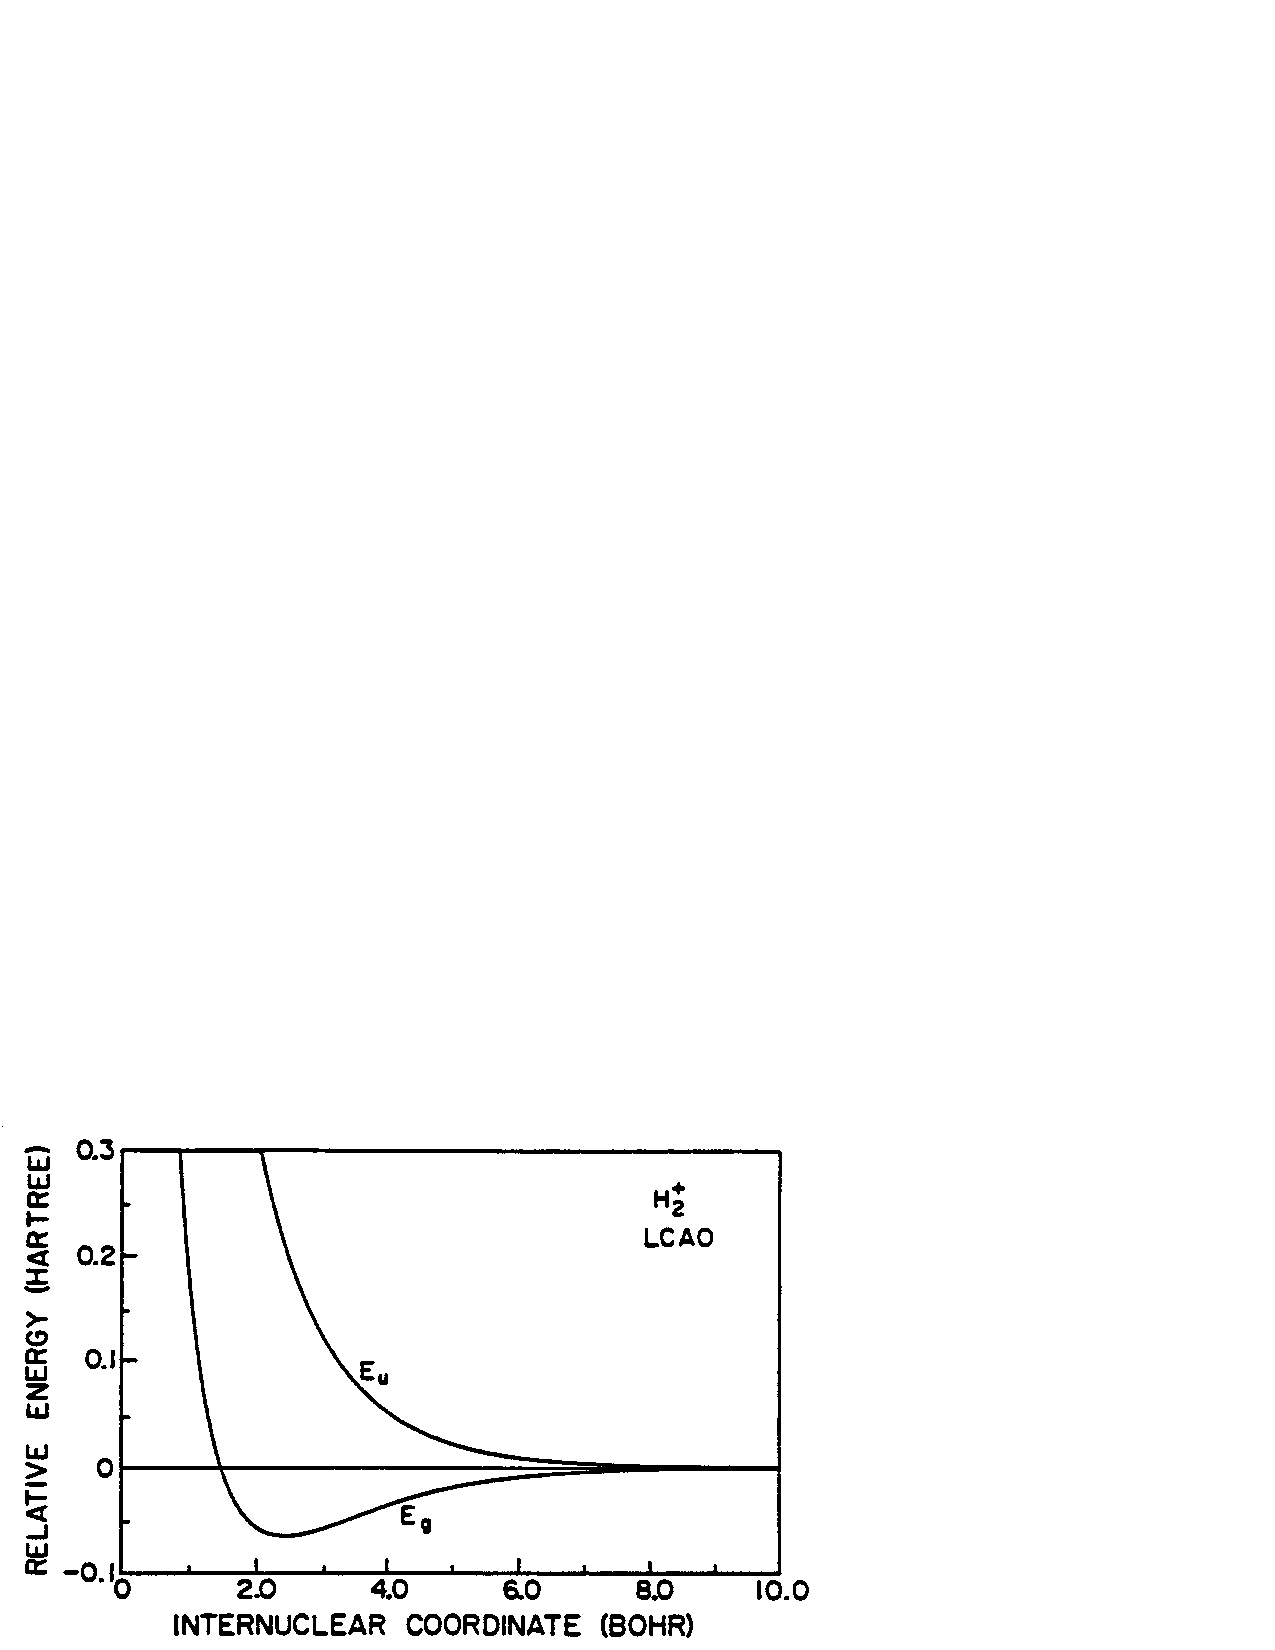
\includegraphics[scale=0.75]{fig2-02}
\caption{The energies of the LCAO wave functions for H$_2^+$.}
\label{fig2-2}
\end{figure}

The energies for the wavefunctions $\varphi_g$ and $\varphi_u$ in
equations (\ref{eqno2-2}) and (\ref{eqno2-3}) are shown as a function
of $R$ in Figure \ref{fig2-2}. Here we see that the $g$ state if
strongly bonding (that is, the energy drops as the nuclei are brought
together), whereas the $u$ state is strongly antibonding (the energy
increases as the nuclei are brought together). The objective of this
section will be to understand the origin of the bonding and
antibonding character exhibited by the $\varphi_g$ and $\varphi_u$
states.


\subsubsection{Electrostatic Energy}

First we consider the electron density,
\begin{equation}
\rho_g = \varphi^2_g = {1 \over D^2_g} \left( \chi_{\ell} + 
\chi_r \right)^2 = {\left( \chi^2_{\ell} + \chi^2_r + 2 
\chi_{\ell} \chi_r \right) \over D^2_g}
\label{eqno2-4}
\end{equation}
Integrating $\varphi^2_g$ over all space must give one electron
\begin{equation}
\langle \varphi^2_g \rangle = 1,
\end{equation}
and similarly
\begin{equation}
\langle \chi^2_{\ell} \rangle = 1
\end{equation}
\begin{equation}
\langle \chi^2_r \rangle = 1
\end{equation}
(recall, these are just the $1s$ orbitals of $H$ atom). Thus, equation
(\ref{eqno2-4}) leads to
\begin{equation}
1 = {1 + 1 + 2S \over D^2_g},
\end{equation}
where $S = \langle \chi_\ell\vert\chi_r \rangle$ is called the overlap
of the two atomic orbitals. Consequently, the normalization condition
of equation (\ref{eqno2-2}) is
\begin{equation}
D_g = \sqrt{2(1+S)}.
\end{equation}

\begin{figure}
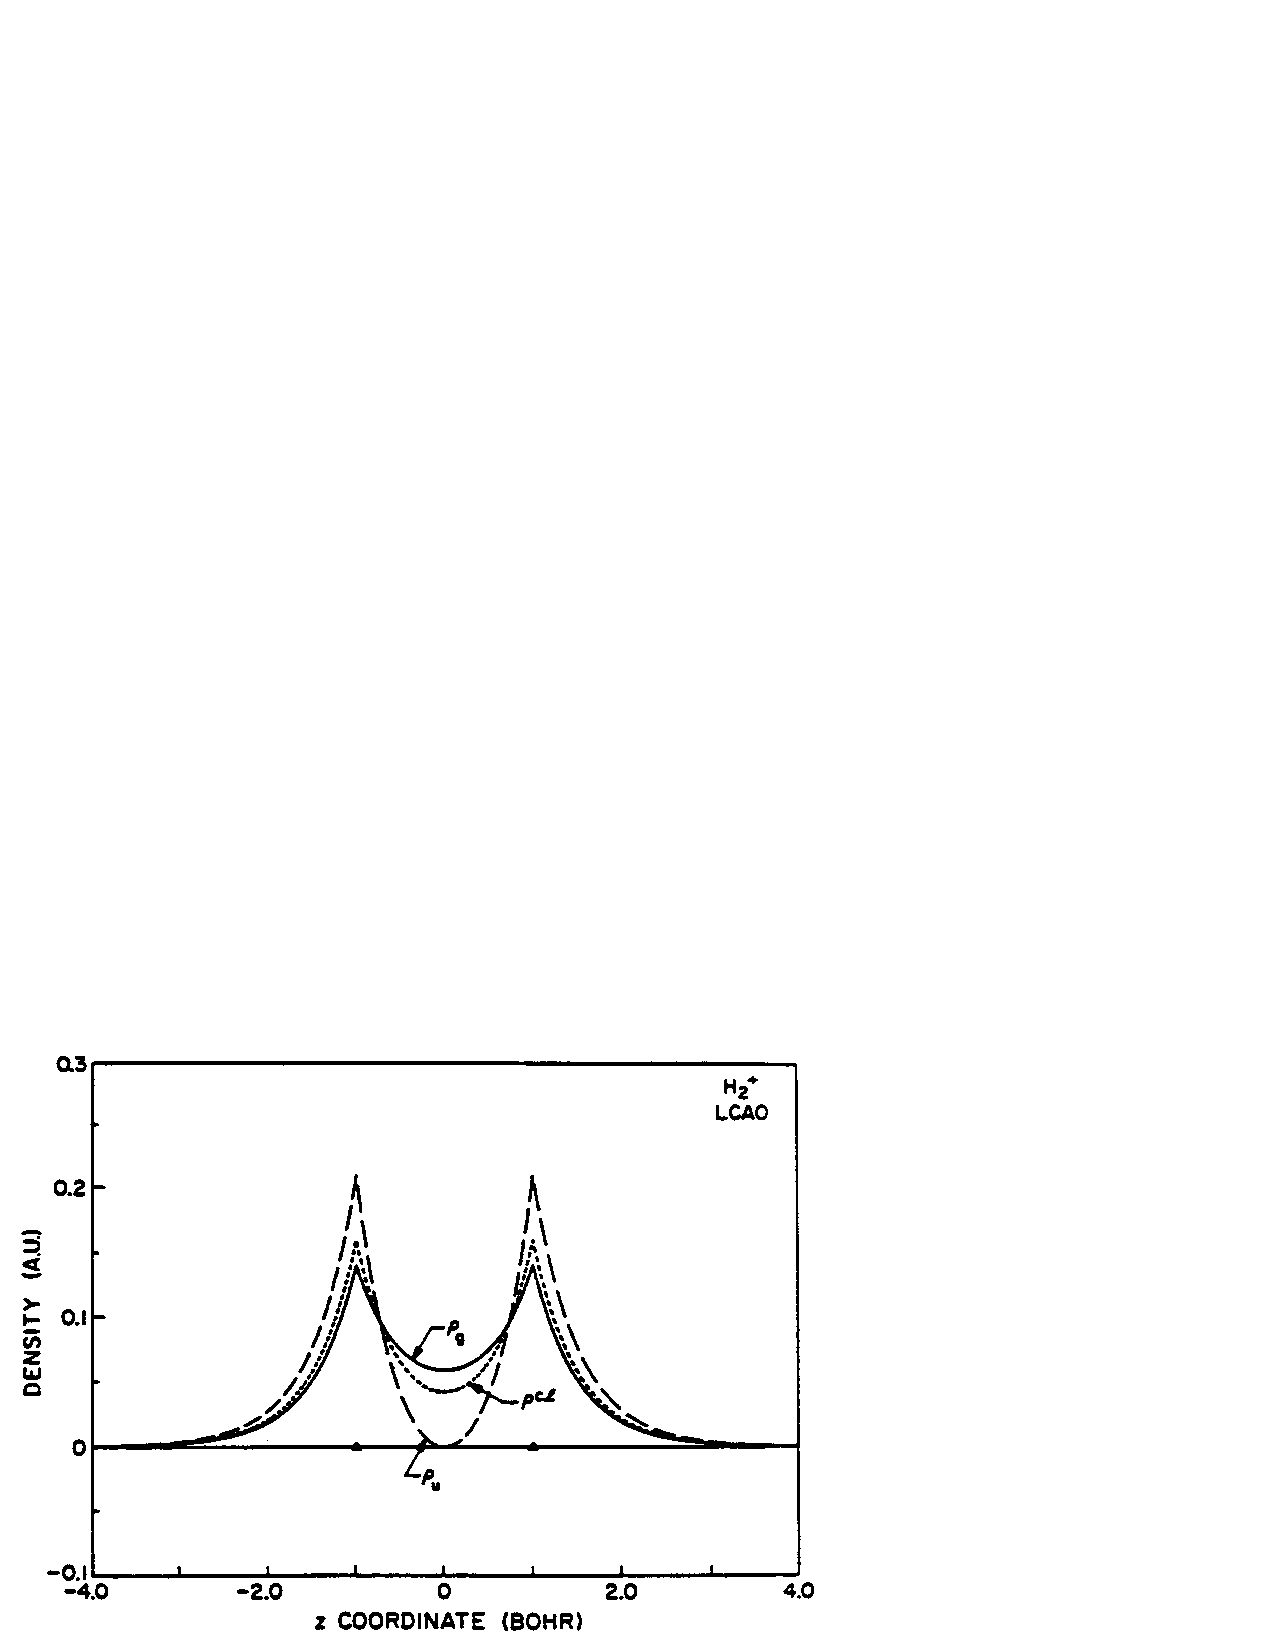
\includegraphics[scale=0.75]{fig2-03}
\caption{The densities $\rho_g$ and $\rho_u$ for the LCAO wave
  functions of H$_2^+$ compared with the superposition of atomic
  densities $\rho^{cl}$.}
\label{fig2-3}
\end{figure}

If there were no interference terms in equation (\ref{eqno2-4}), the
density would be
\begin{equation}
\rho^{cl} = {1 \over 2} \left( \chi^2_{\ell} + \chi_r^2 \right)
\end{equation}
where the factor of 1/2 leads to the required condition of $\langle
\rho^{cl} \rangle = 1$.  But because of the interference terms the
density near the bond midpoint is increased, as shown in Figure
\ref{fig2-3}. This result has given rise to the prevalent idea that
the chemical bond arises from the increase in the electron charge
density in the bond region. The idea is that an electron in between
the nuclei attracts both nuclei, holding them together to form the
chemical bond, $p^+e^-p^+$. This reasoning is false, as will now be
demonstrated.  The total potential energy is given by
\begin{equation}
V(r) = - {e^2 \over r_a} - {e^2 \over r_b} + {e^2 \over R},
\end{equation}
as sketched in Figure \ref{fig2-4}.  Here we see that the best place
for the electron (lowest energy) is at a nucleus ($r_a = 0$ or $r_b =
0$) not at the bond midpoint. From Figure \ref{fig2-3} we observe that
the increase in charge at the bond midpoint is at the expense of
charge near the nucleus. Thus, in forming a bond, the charge is
transferred from a low energy region, near the nucleus, to a high
energy region, the bond midpoint. An effect that should operate
against bond formation. Indeed, this is the case, as shown in Figure
\ref{fig2-5}, where
\begin{equation}
V_g = \langle \varphi^2_g V ( {\bf r} ) \rangle
\end{equation}
is the total potential energy for the $\varphi_g$ wavefunction.

\begin{figure}
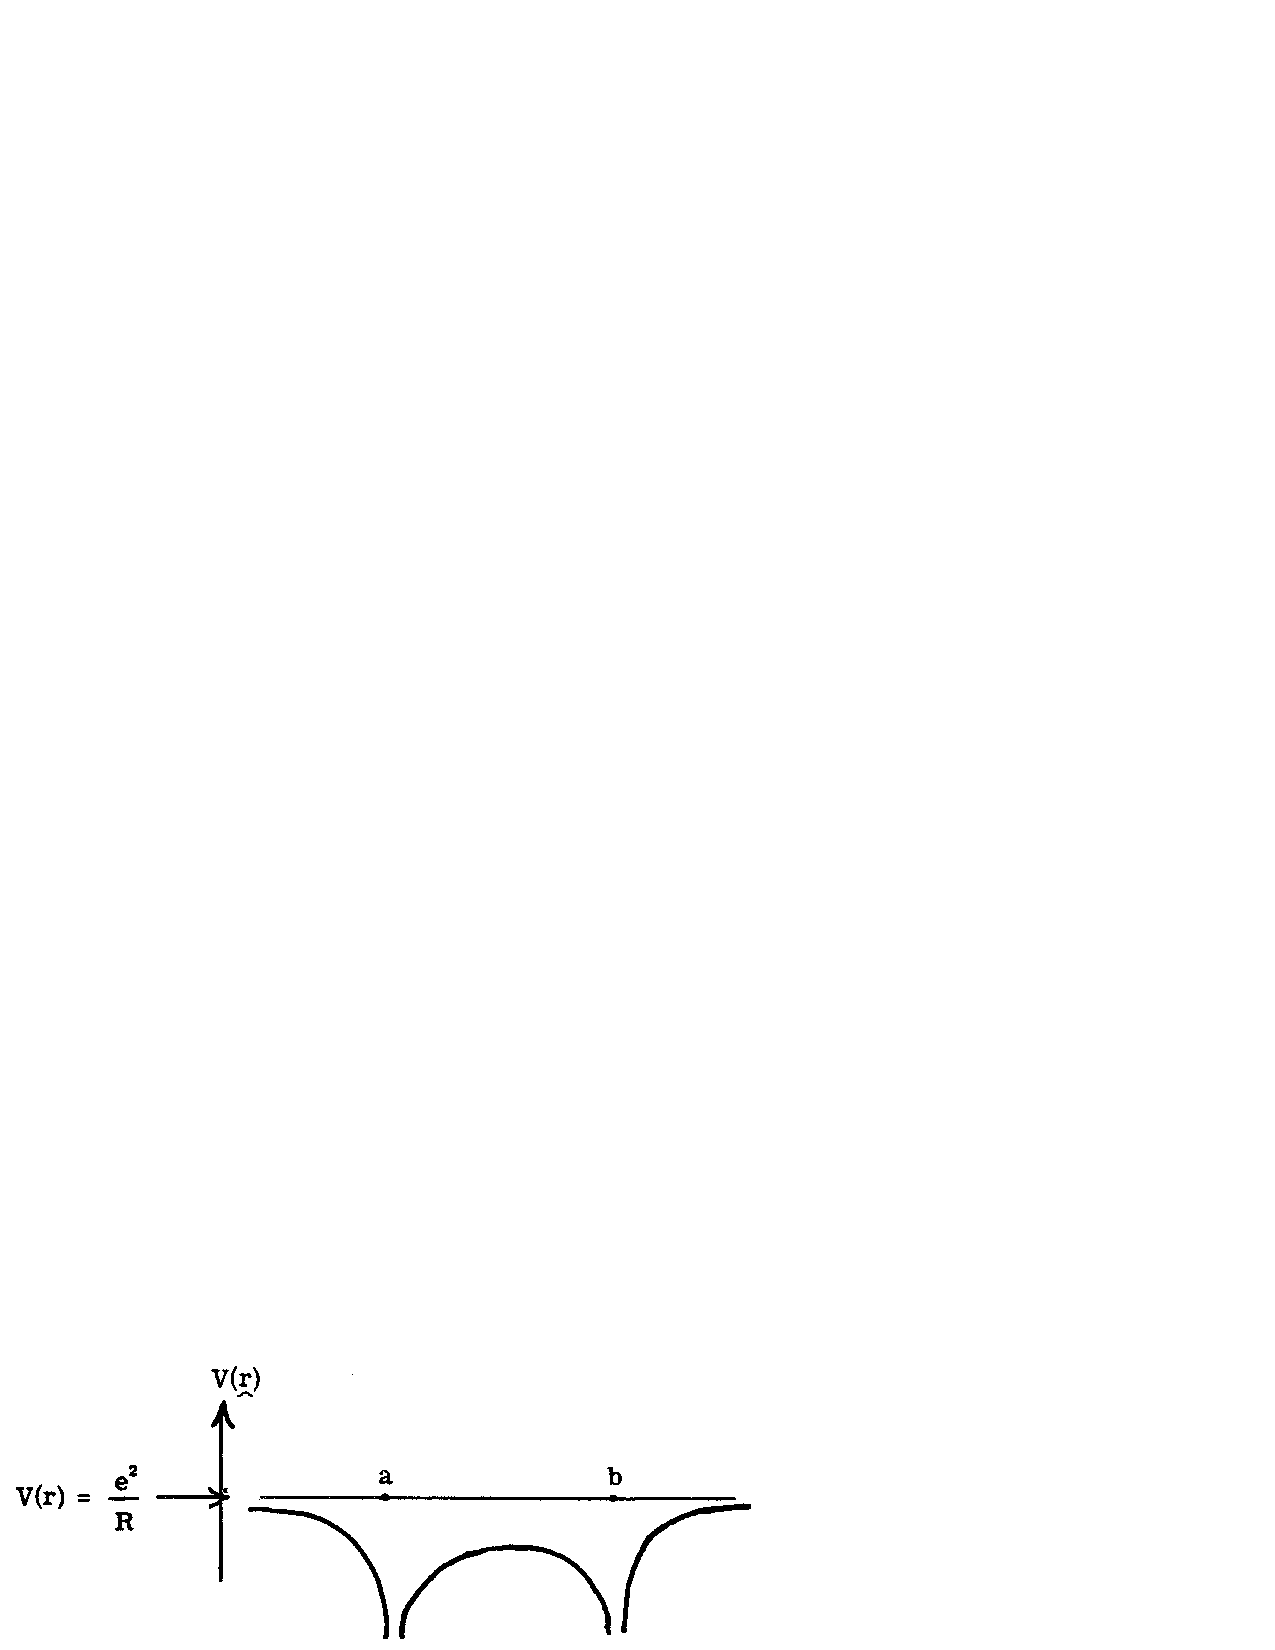
\includegraphics[scale=0.75]{fig2-04}
\caption{The nuclear attraction potential $V(r)$ for H$_2^+$.}
\label{fig2-4}
\end{figure}

\begin{figure}
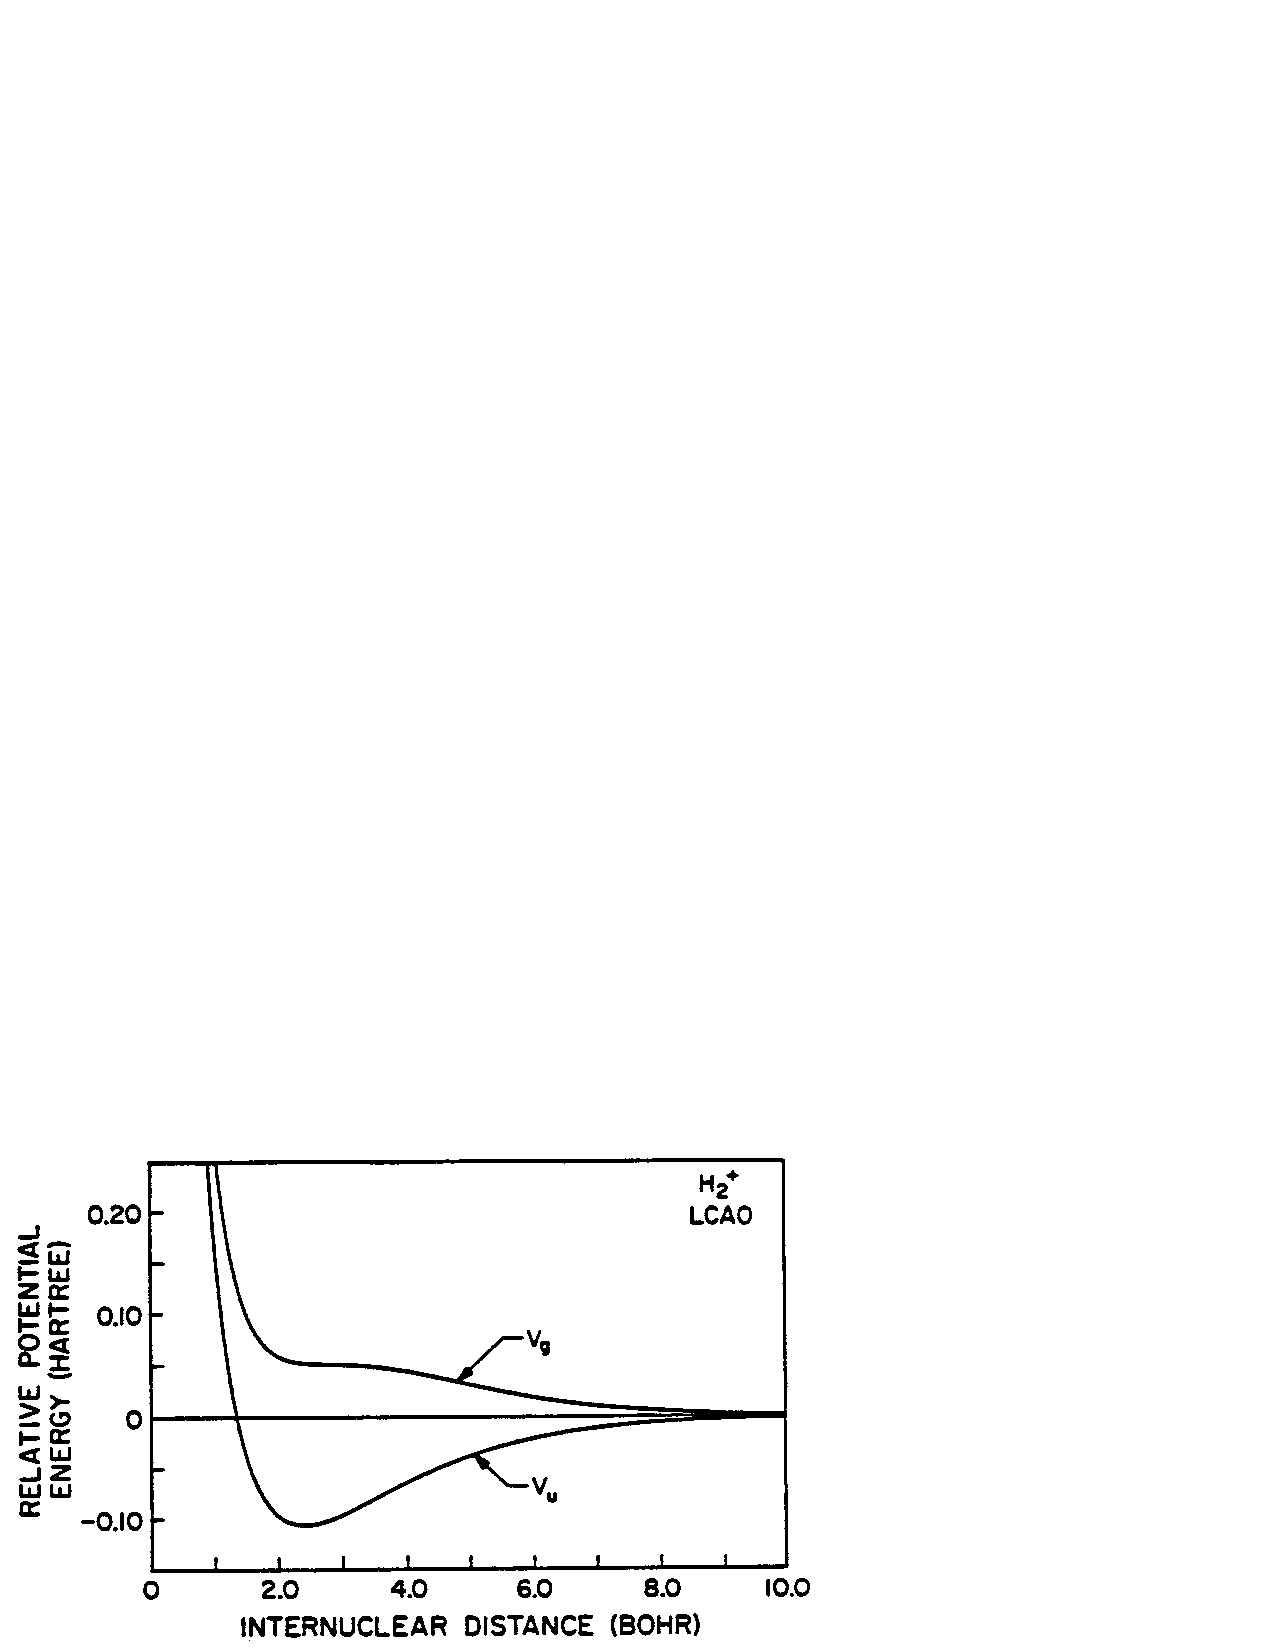
\includegraphics[scale=0.75]{fig2-05}
\caption{The relative potential energies $V_g$ and $V_u$ for the LCAO
  wave functions of H$_2^+$. The absolute values are obtained by
  noting that $V_g = V_u = -1.0$ at $R=\infty$.}
\label{fig2-5}
\end{figure}

Our conclusion then is that the transfer of electron charge into the
bond region leads to repulsive electrostatic interactions. The fact
that the bonding state leads to such a transfer indicates that the
origin of the bond lies in the other contribution to the energy, the
kinetic energy, as will be discussed next.

\subsubsection{Kinetic Energy}

\begin{figure}
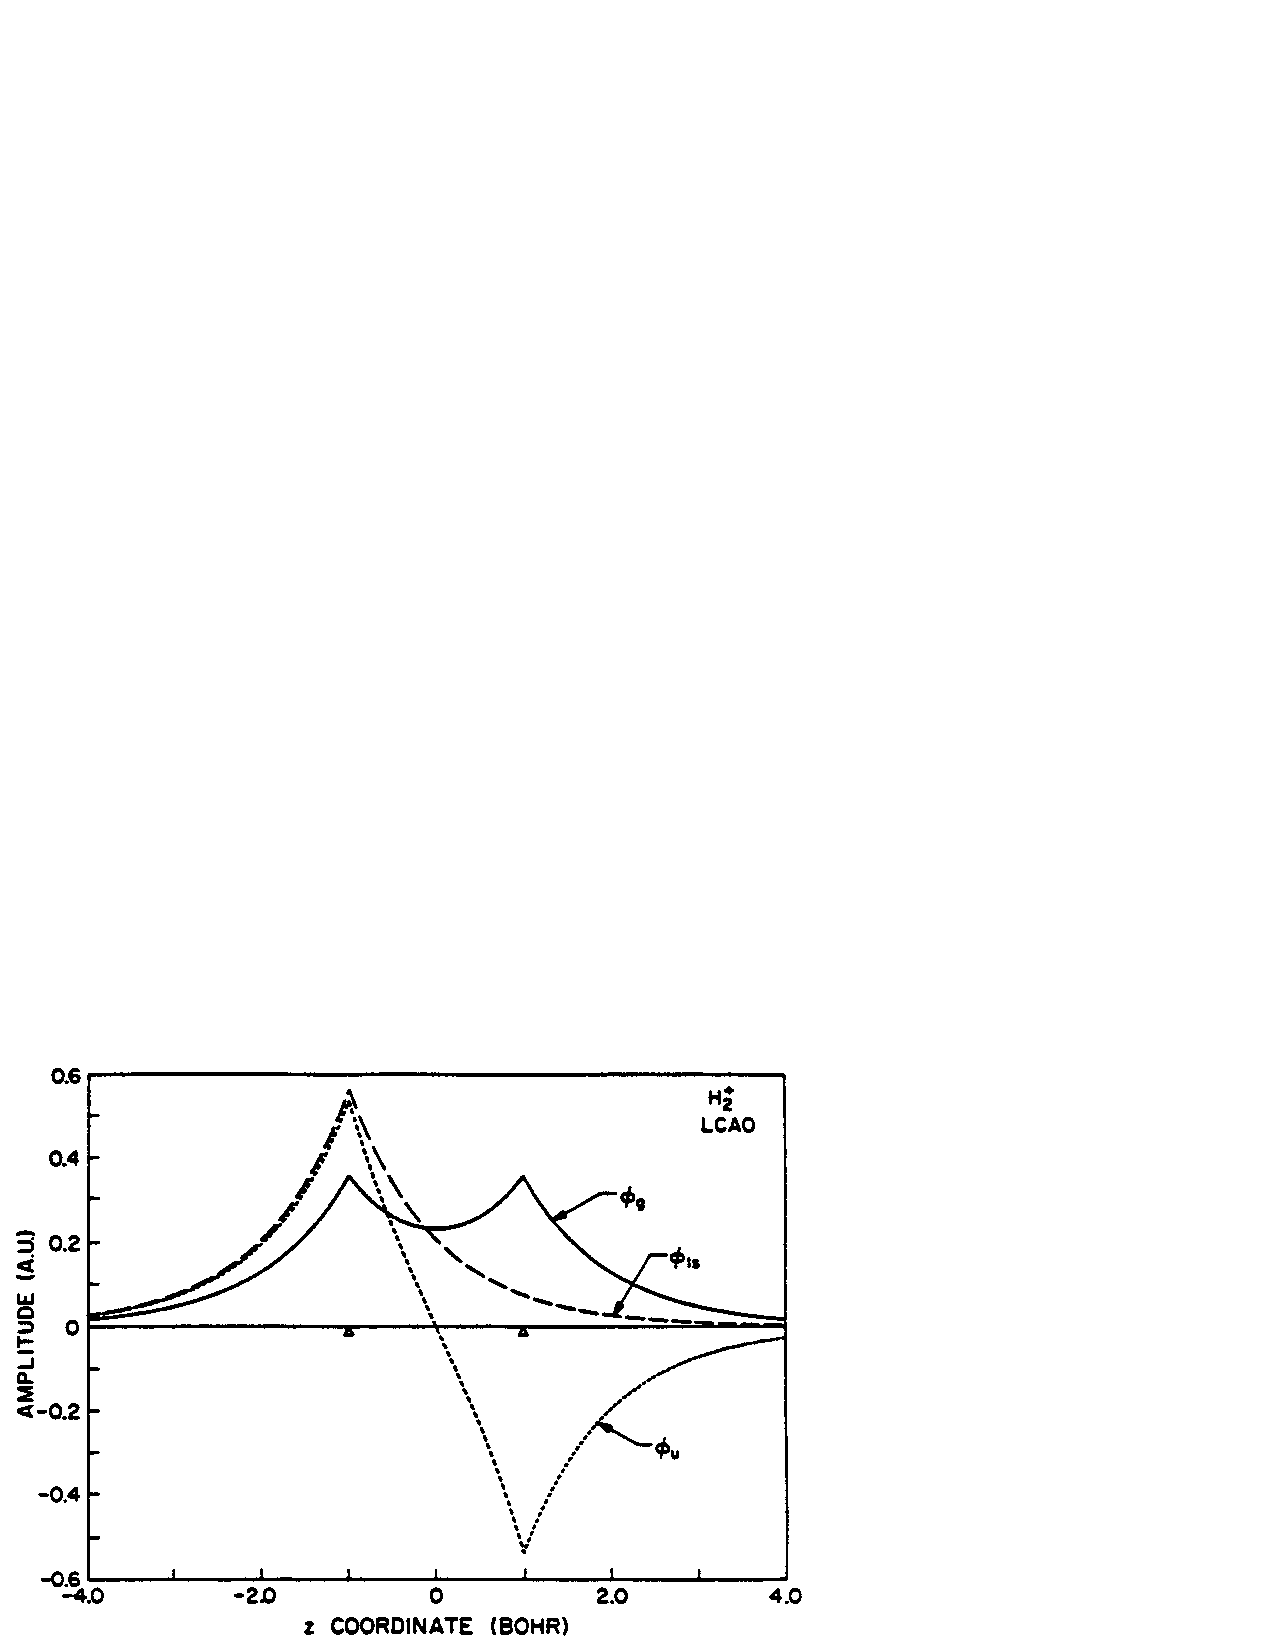
\includegraphics[scale=0.75]{fig2-06}
\caption{Comparison of the $\varphi_g$ and $\varphi_u$ LCAO's of
  H$_2^+$ with the hydrogen orbital, $\varphi_{1s}$. All wave
  functions have been normalized.}
\label{fig2-6}
\end{figure}

A qualitative prediction of changes in kinetic energy upon bond formation 
is easy. The kinetic energy is the (average) square of the gradient of the 
wavefunction
\begin{equation}
T = \left( {\hbar^2 \over 2m} \right) \langle \vert \nabla \psi 
\vert^2 \rangle.
\end{equation}
Superimposing two atomic orbitals symmetrically, as in $\varphi_g$,
leads to a large decrease in the slope in the bond region, see Figure
\ref{fig2-6}, and hence, a large decrease in the kinetic energy, see
$T_g$ in Figure \ref{fig2-7},
\begin{equation}
 T_g = \left( {\hbar^2 \over 2m} \right) \langle \vert \nabla \varphi_g 
  \vert^2 \rangle
\end{equation}
resulting in a strong bond. On the other hand, the antisymmetric
combination in $\varphi_u$ leads to a large increase in the slope in
the bond region (see Figure \ref{fig2-6}) and hence, the kinetic
energy opposes bond formation (see $T_u$ of Figure \ref{fig2-7}).

\begin{figure}
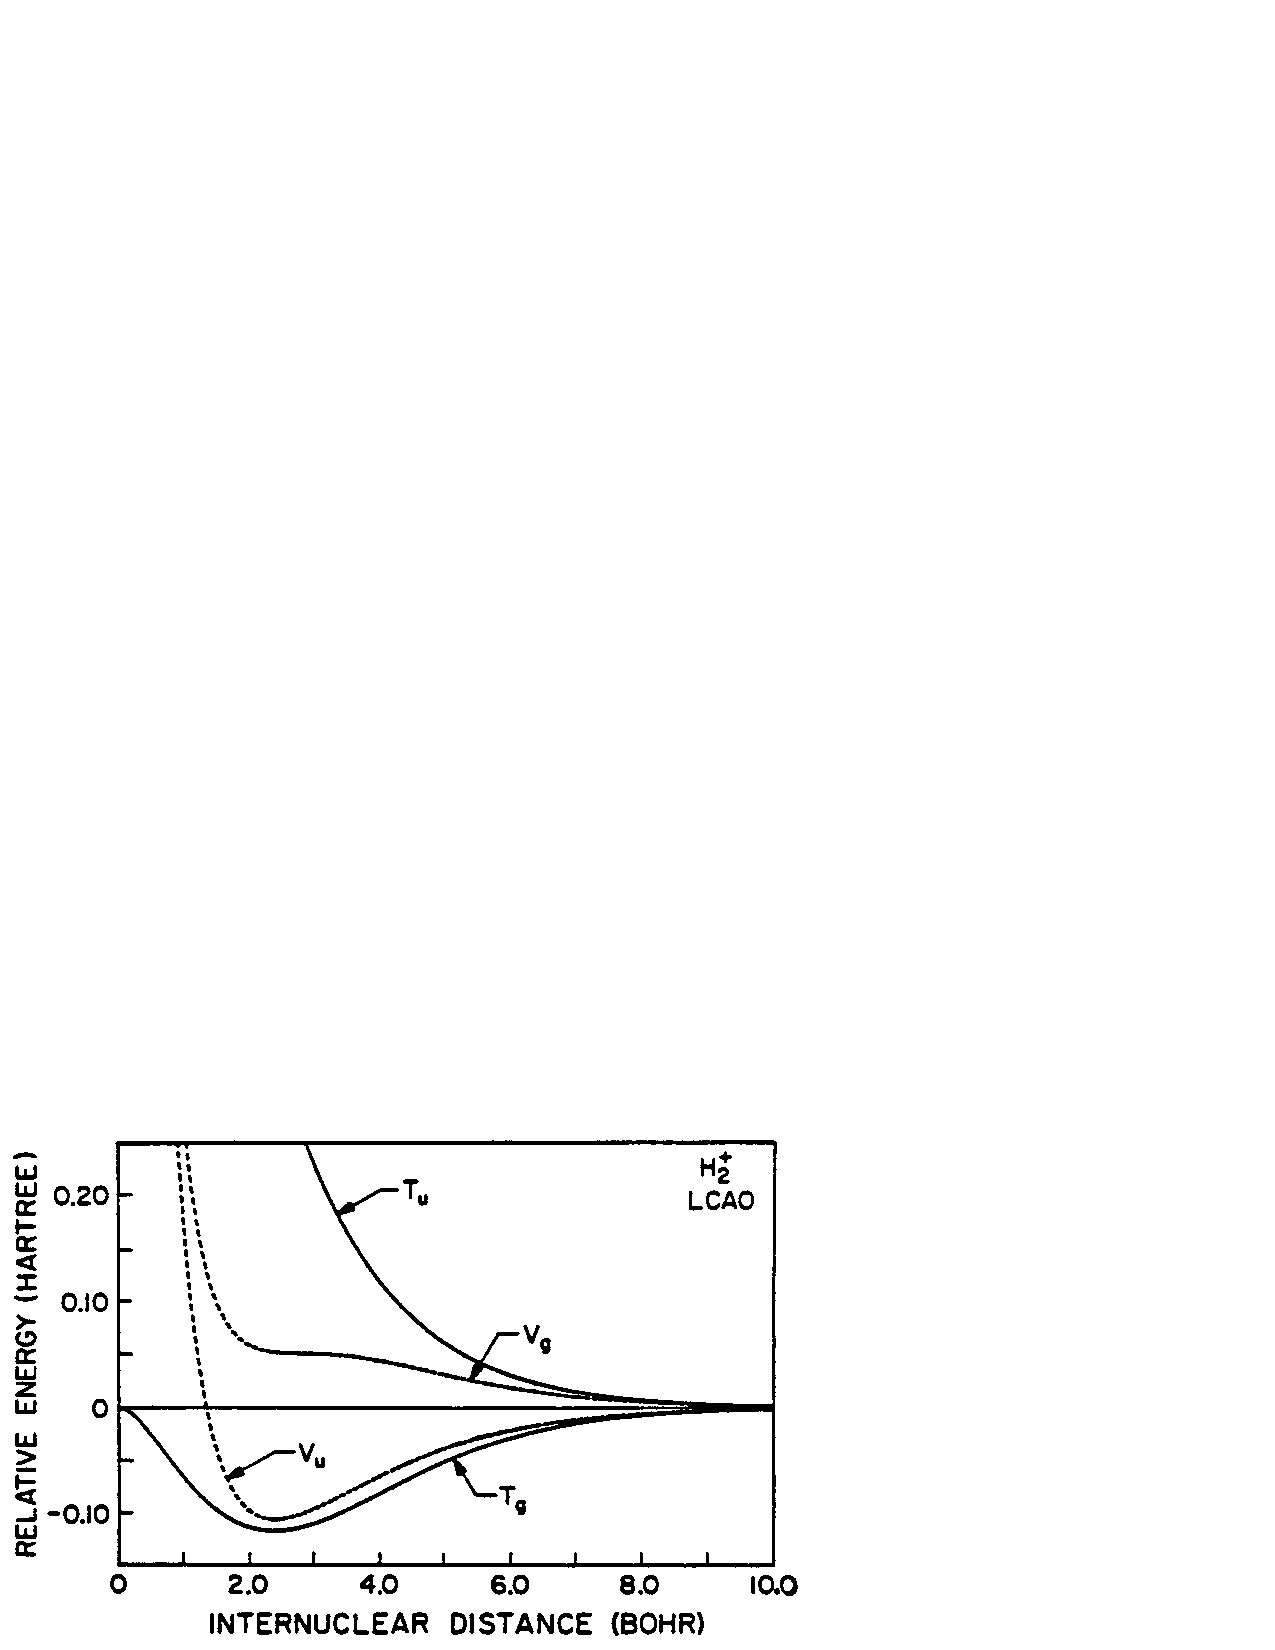
\includegraphics[scale=0.75]{fig2-07}
\caption{The changes in the total kinetic and potential energies for
  the $g$ and $u$ LCAO wave functions of H$_2^+$. The actual values at
  $R=\infty$ are $T_u(\infty)=T_g(\infty)=+\frac{1}{2}$ and
  $V_u(\infty)=V_g(\infty)=-1$.} 
\label{fig2-7}
\end{figure}

The resulting total energies are given in Figure
\ref{fig2-2}, where we see that $\varphi_g$ is strongly bonding, while
$\varphi_u$ is strongly antibonding.

\subsection{Bonding to $p$ Orbitals}

Above we found that it is the change in the kinetic energy that
dominates the energy changes in the LCAO description. Basically, if
two atomic orbitals are superimposed so that no new nodal planes are
created, as in Figure \ref{fig2-8}(a), then the kinetic energy drops
significantly due to the decrease in the gradient of the orbital in
the internuclear region. This is a general phenomenon and depends only
on the fact that in the bond region the gradients of the atomic
orbitals are in opposite directions (contragradient) so that 
(symmetric) superposition of the orbitals leads to a decrease in the
gradients.

\begin{figure}
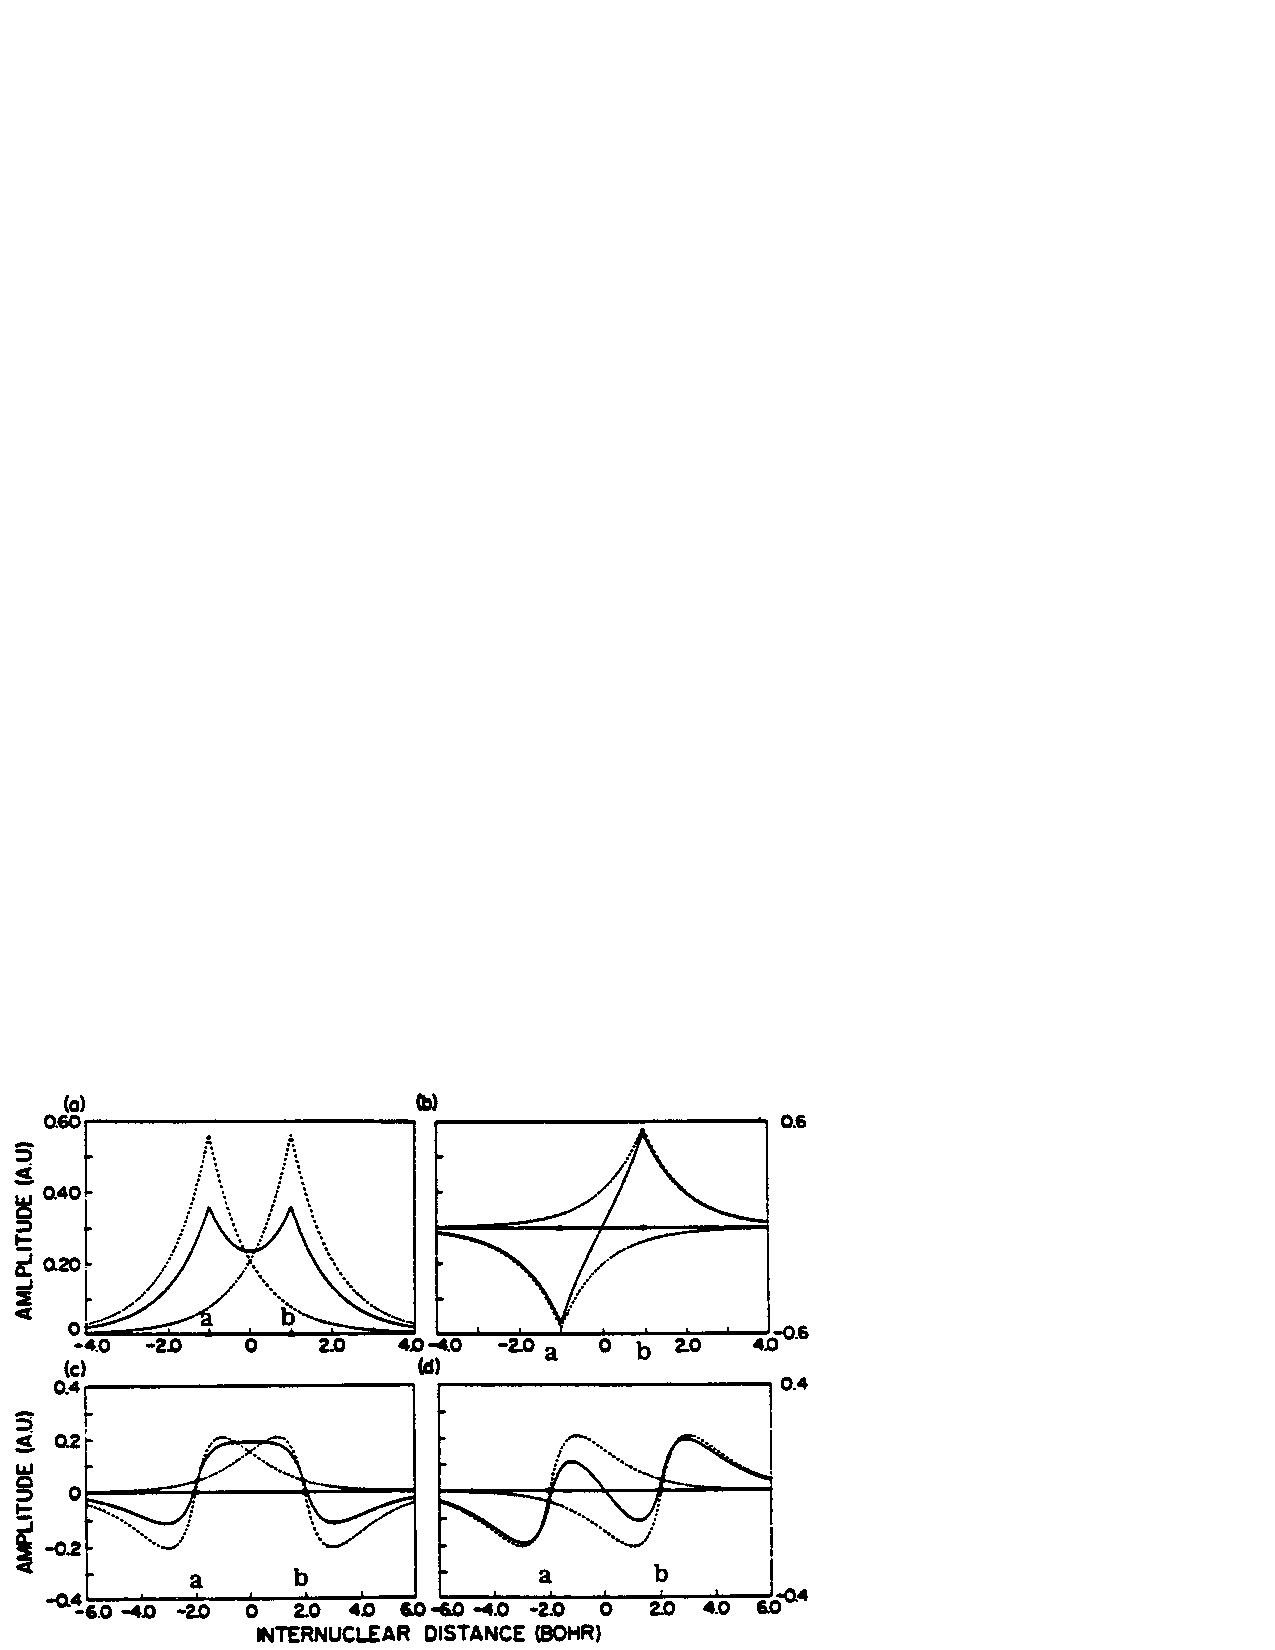
\includegraphics[scale=0.75]{fig2-08}
\caption{(a,b) Symmetric an antisymmetric superposition of $1s$ atomic
orbitals. (c,d) Symmetric and antisymmetric superposition of $2p_x$
orbitals (oriented along the axis).}
\label{fig2-8}
\end{figure}

\begin{figure}
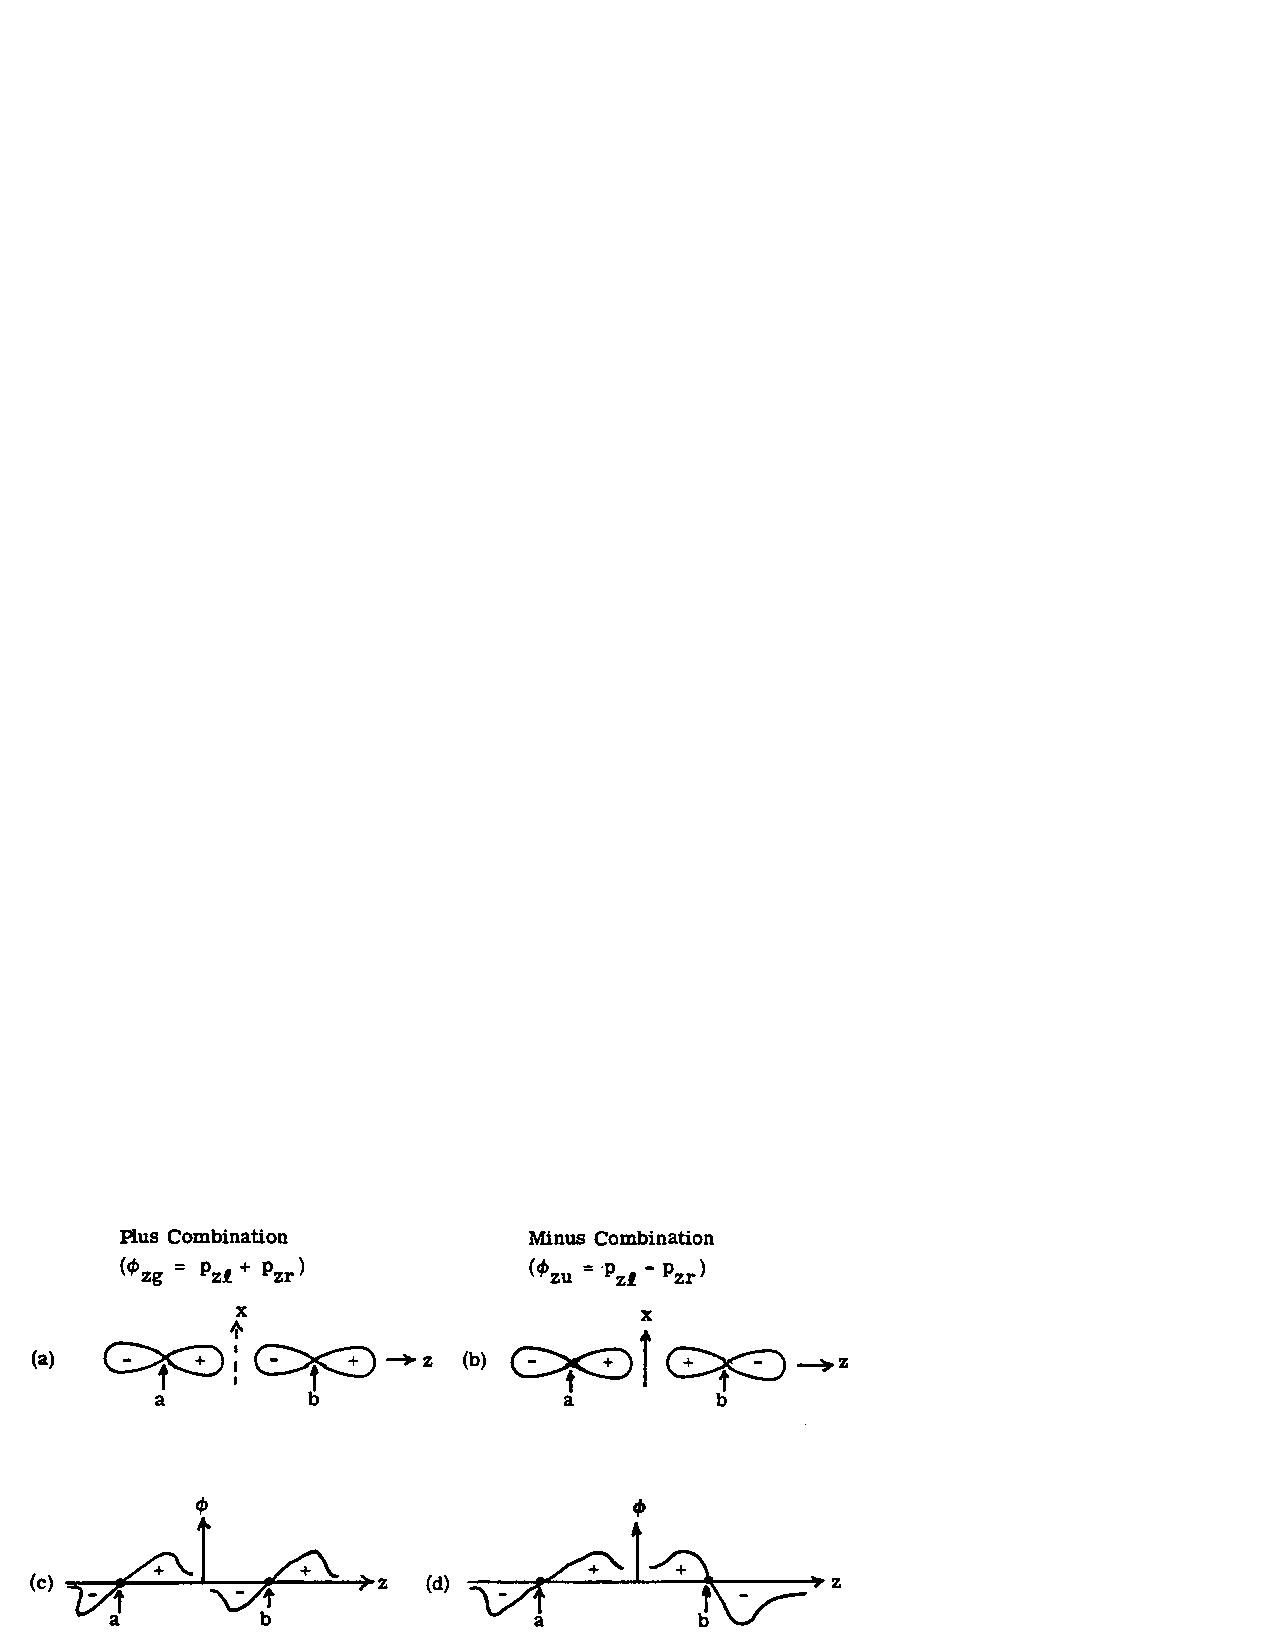
\includegraphics[scale=0.75]{fig2-09}
\caption{Bonding between $p_x$ orbitals. (a) and (b) are schematic
  diagrams of the shape of the orbitals in the $xz$-plane. (c) and (d)
  are plots of the orbitals along the $z$-axis.}
\label{fig2-9}
\end{figure}

These results are not limited to superimposing 1s orbitals. Consider,
for example, a bond between $p_z$ orbitals on two atoms, assuming $z$
to be the internuclear axis, as in Figure \ref{fig2-9}.  The plus
combination, $\varphi_{zu} = p_{z \ell} + p_{zr}$, leads to a new nodal
plane, higher gradients, and antibonding, as shown in Figure
\ref{fig2-9}(d). Meanwhile the minus combination, $\varphi_{zu} = p_{z
\ell} - p_{zr}$, leads to lower gradients and bonding, as shown in
Figure \ref{fig2-9}(c).  Similarly, bonding of the $p_x$ orbitals
leads to Figure \ref{fig2-10}. Now the minus combinationi
$\varphi_{xu} = p_{x \ell} - p_{xr}$ leads to a new nodal plane and
antibonding. While the plus combinations, $\varphi_{xg} = p_{x \ell} -
p_{xr}$, leads to bonding.

\begin{figure}
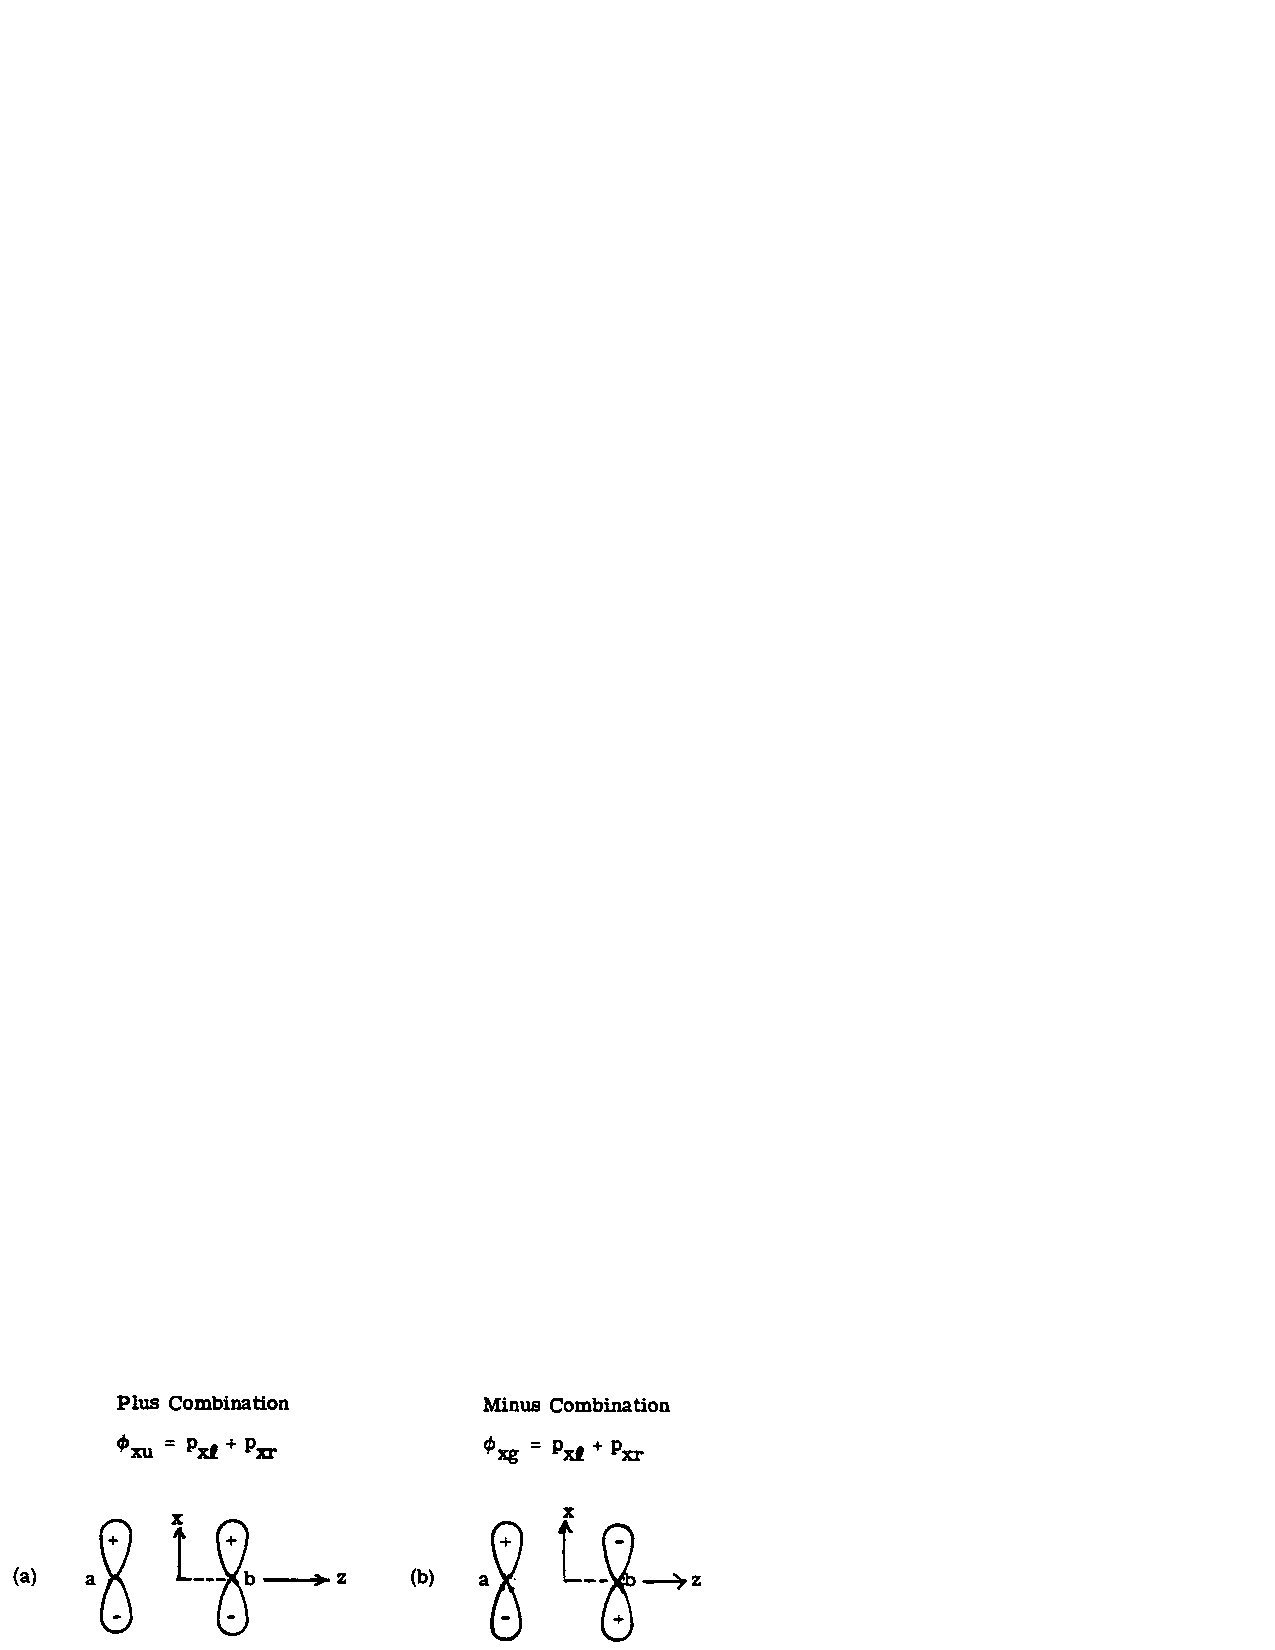
\includegraphics[scale=0.75]{fig2-10}
\caption{Bonding between $p_x$ orbitals.}
\label{fig2-10}
\end{figure}

\subsection{The Optimum Distance for Bonds}

There is a natural optimum range for the effects that dominate 
bonding. First, if $R$ is very large, near $\infty$, there is a large 
region in which the gradient is decreased. However,
at each point, one or the other of the two orbitals has a very small 
gradient, so that the decrease in the gradient is very small (and goes 
to zero as $R \rightarrow \infty$). The result is a small
bonding contribution for large $R$.

Secondly, if $R$ is very small, near 0, there is a large decrease in
the gradient.  However, the region of this large decrease is only the
small region between the nuclei, which goes to zero as $R \rightarrow
0$. The latter effect is illustrated in Figure \ref{fig2-11}, where
the left side is for $R$ near optimum and the right side is for small
$R$. Figure \ref{fig2-11} illustrates the effect of $R$ on the
contragradience of orbitals.  In each case, the $R$ for the left case
is near optimum, while the $R$ for the right case, is too small.

\begin{figure}
\begin{center}
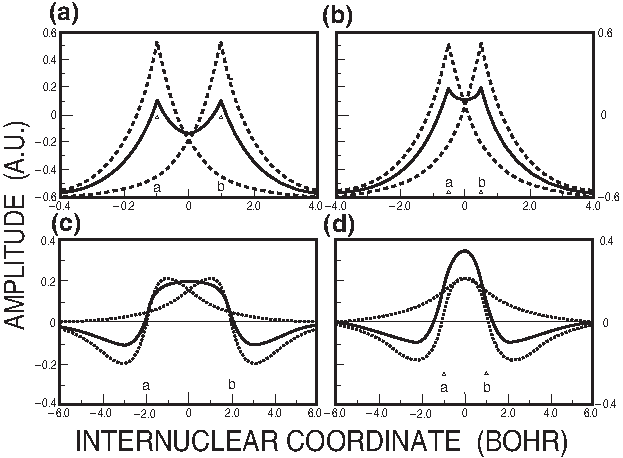
\includegraphics[scale=0.75]{fig2-11}
\end{center}
\caption{Illustrations of the effect of $R$ on the contragradience of
  orbitals. In each case the $R$ for the left case is near optimal,
  whereas the $R$ for the right case is too small.}
\label{fig2-11}
\end{figure}

Thus, the optimum bond is formed at an intermediate distance where the 
gradients are large and opposite (contragradient) for a large region. For 
the hydrogen $1s$ orbital, the optimum distance is about $2a_0$, which 
is just the sum of the atomic radii. For a $p$ orbital,
the optimum decrease in the gradient occurs when the outer lobes are separated
significantly, as illustrated in Figure \ref{fig2-11}(c).

\subsection{Symmetry Considerations}

The H$^+_2$ molecule has a great deal of symmetry. In quantum mechanics,
symmetry in the molecule generally leads to symmetry in the wavefunction, and
knowledge of these symmetries, can aid us in both solving for the 
wavefunctions and in reasoning qualitatively about them. For the time being, 
we will concern ourselves with only one of the symmetries in H$^+_2$, 
namely, the inversion symmetry.

\subsubsection{The Hamiltonian}
    
First, we need to consider the form of the Hamiltonian for H$^+_2$
Using the coordinate system of Figure \ref{fig2-1}, the full
Hamiltonian for H$^+_2$ is
\begin{equation}
{\hat H} \left( \mathrm{H}^+_2 \right) = - {\hbar^2 \over 2M_a} \nabla^2_a - 
{\hbar^2 \over 2M_b} \nabla^2_b - {\hbar^2 \over 2m} \nabla^2_1 - 
{Z_ae^2 \over r_a} - {Z_be^2 \over r_b} + {Z_aZ_be^2 \over R}
\label{eqno2-5}
\end{equation}
We will simplify equation (\ref{eqno2-5}) by assuming the nuclear
masses to be infinitely heavy ($M_a = M_b = \infty$) by taking the
nuclear charges as unity (as appropriate for H$^+_2$) and by using
atomic units ($\hbar = m = e = 1$). This reduces equation
(\ref{eqno2-5}) to
\begin{equation}
{\hat H} \left( \mathrm{H}^+_2 \right) = - {1 \over 2} \nabla^2_1 - {1
\over r_a} - {1 \over r_b} + {1 \over R}.
\end{equation}
We will group together all the terms depending upon the coordinates of one
(and only one) electron as
\begin{equation} 
h(1) = - {1 \over 2} \nabla^2_1 + v(1)
\end{equation}
referred to as the \emph{one-electron Hamiltonian}, where
\begin{equation}
v(1) = - {1 \over r_a} - {1 \over r_b}
\label{eqno2-6}
\end{equation}
is the nuclear attraction term, arising from the attractive 
electron-nuclear interactions.   This leads to
\begin{equation}
{\hat H} \left( \mathrm{H}^+_2 \right) = h ( 1 ) + {1 \over R}.
\label{eqno2-7}
\end{equation}

The exact electronic wavefunction of H$^+_2$ is obtained by solving
\begin{equation}
{\hat H} \varphi ( 1 ) = E \varphi ( 1 ) ,
\label{eqno2-8}
\end{equation}
where $H$ is given by equation (\ref{eqno2-7}). Substituting equation
(\ref{fig2-7}) into equation (\ref{eqno2-8}) and rearranging, we
obtain
\begin{equation}
h \varphi = \epsilon \varphi,
\label{eqno2-9}
\end{equation}
where
\begin{equation}
\epsilon = E - {1 \over R}
\end{equation}
is referred to as the electronic energy.  Although equation
(\ref{eqno2-9}) may appear to involve only the electronic coordinates
{\bf r}, the internuclear coordinate $R$ is involved implicitly, since
it determines the spacing of the attractive terms in $v$,
(\ref{eqno2-6}). In solving for the wavefunction of H$^+_2$, we choose
an $R$ and solve equation (\ref{eqno2-9}) to obtain the electronic
wavefunction $\varphi ( {\bf r})$ and the electronic energy
$\epsilon$. We then chose a new $R$ and again solve equation
(\ref{eqno2-7}), obtaining a new $\varphi ( {\bf r})$ and an
electronic energy $\epsilon$, each of which is parametrically
dependent upon $R$. This procedure is referred to as the
Born-Oppenheimer approximation.

\subsubsection{Inversion Symmetry}
    
\begin{figure}
\begin{center}
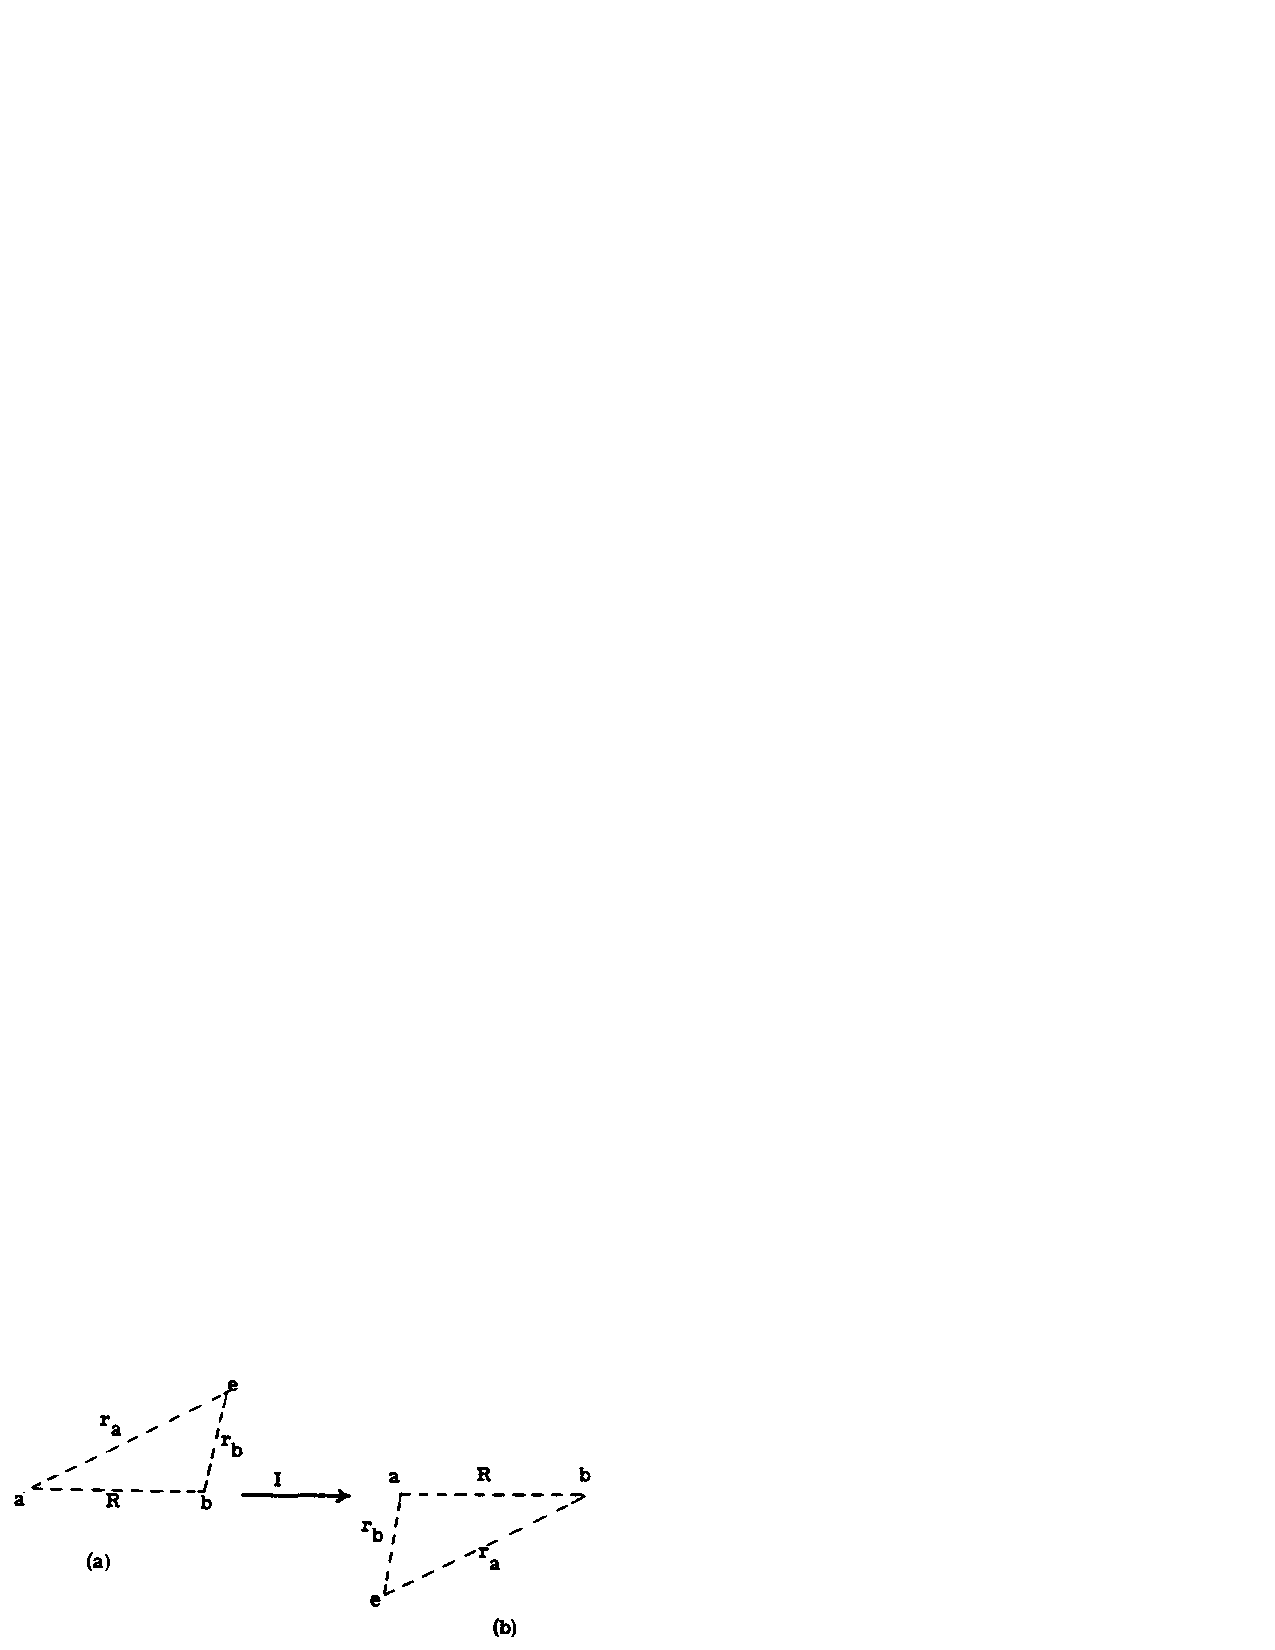
\includegraphics[scale=0.75]{fig2-12}
\end{center}
\caption{The effect of inverting the coordinates of the electron.}
\label{fig2-12}
\end{figure}

The operation of inversion through the origin of a coordinate system
leads to the changes $x \rightarrow - x$, $y \rightarrow -y$, and $z
\rightarrow -z$ in the coordinates, and will be denoted as ${\hat
I}$. Taking the origin of the coordinate systems as the bond midpoint
in Figure \ref{fig2-1}, the inversion of the coordinates of the
electron leads to Figure \ref{fig2-12}.  The electron is now $r_a$
from the right nucleus in Figure \ref{fig2-12}(b), and $r_b$ from the
left nucleus as shown in Figure \ref{fig2-12}(a).  However, since the
nuclear charges are the same, the potential terms in the Hamiltonian
are the same.
    
Upon inversion, the kinetic energy terms in ${\hat H}$ are also unchanged
\begin{equation}
\nabla^2 = {\partial^2 \over \partial x^2} + {\partial^2 \over 
\partial y^2} + {\partial^2 \over \partial z^2} \rightarrow 
{\partial^2 \over \partial (-x)^2}  + {\partial^2 \over \partial 
(-y)^2} + {\partial^2 \over \partial (-z)^2} = \nabla^2,
\end{equation}
and hence, the Hamiltonian is invariant upon inversion of the electronic 
coordinate, through the bond midpoint.
    
Now consider that we have solved equation (\ref{eqno2-8}) to obtain
eigenstates of H$^+_2$
\begin{equation}
{\hat H} \varphi = E \varphi ,
\label{eqno2-10}
\end{equation}
and apply ${\hat I}$ to both sides of equation (\ref{eqno2-10}). The
result is
\begin{equation}
{\hat I} ( {\hat H} \Phi ) = E ( {\hat I} \varphi ) ,
\end{equation}
which we could write as
\begin{equation}
{\hat H} ( - {\bf r} ) \varphi (- {\bf r} ) = E \varphi ( - {\bf 
r} ),
\label{eqno2-11}
\end{equation}
indicating the result of inversion. But ${\hat H}$ is invariant 
under ${\hat I}$,
\begin{equation}
{\hat H}(-{\bf r}) = {\hat H} ({\bf r})
\end{equation}
so that equation (\ref{eqno2-11}) becomes
\begin{equation}
{\hat H} ( {\bf r} ) \varphi ( - {\bf r} ) = E \varphi ( - {\bf r} )
\end{equation}
or
\begin{equation}
{\hat H} ( {\bf r} ) ( {\hat I} \varphi ) = E ( {\hat I} \varphi 
).
\label{eqno2-12}
\end{equation}

Equations (\ref{eqno2-10}) and (\ref{eqno2-12}) state that $\varphi$
and ${\hat I} \varphi$ are each eigenfunctions of exactly the same
Hamiltonian with exactly the same energy. There are two possibilities
here. The state is nondegenerate, in which case ${\hat I} \varphi$ and
$\varphi$ must be proportional to each other. Or the state is
degenerate, in which case ${\hat I} \varphi$ and $\varphi$ may be
linearly independent function, i.e., not proportional.
    
First we consider that the state is nondegenerate. In this case,
\begin{equation}
{\hat I} \varphi = \lambda \varphi,
\label{eqno2-13}
\end{equation}
where $\lambda$ is some constant. But applying ${\hat I}$ twice leads 
to $x \rightarrow x$, $y \rightarrow y$, and $z \rightarrow z$. Thus,
must return the original function
\begin{equation}
{\hat I}^2 \varphi ( {\bf r} ) = {\hat I} \varphi ( - {\bf r} ) = 
\varphi ( {\bf r} ).
\label{eqno2-14}
\end{equation}
Whereas applying ${\hat I}$ to equation (\ref{eqno2-13}) leads to
\begin{equation}
{\hat I}^2 \varphi = \lambda {\hat I} \varphi
\end{equation}
and using equation (\ref{eqno2-13}) on the right side, leads to
\begin{equation}
{\hat I}^2 \varphi = \lambda^2 \varphi.
\label{eqno2-15}
\end{equation}
Combining equations (\ref{eqno2-14}) and (\ref{eqno2-15}), leads to
\begin{equation}
\varphi ( r ) = \lambda^2 \varphi (r)
\end{equation}
or 
\begin{equation}
\lambda^2 = 1,
\end{equation}
leading to 
\begin{equation}
\lambda = \pm 1.
\end{equation}
That is, nondegenerate states of H$^+_2$ must be either symmetric
under inversion ($\lambda = + 1$) or antisymmetric ($\lambda = -1$).
Wavefunctions with these symmetries are denoted with $g$ for
\emph{gerade} or \emph{even} in German, or $u$ for \emph{ungerade} or
\emph{uneven}, as in $\varphi_g$ or $\varphi_u$.

Consider now the case of a degenerate state with ${\hat I} \varphi$
not proportional to $\varphi$.  We can form two new functions,
$\varphi_g = \varphi + {\hat I} \varphi$, and $\varphi_u = \varphi -
{\hat I} \varphi$, such that each function is still an eigenfunction
of $H$, with the same energy, $H \varphi_g = E \varphi_g$ and $H
\varphi_u = E \varphi_u$ but such that one function is gerade ${\hat
I} \varphi_g = \varphi_g$, while the other is ungerade ${\hat I}
\varphi_u = - \varphi_u$.  Thus, in this case, also the eigenfunctions
of $H$ are $g$ or $u$.
 
If a certain state is doubly-degenerate with wavefunctions 
$\varphi_a$ and $\varphi_b$, then
starting with just one function, say $\varphi_a$, we generate both a $g$ 
function and a $u$ function, $\varphi_{ga} = \varphi_a + I \varphi_a$ 
and  $\varphi_{ua} = \varphi_a + I \varphi_a$.  If these functions
are both nonzero, then $\varphi_b$ will be a linear
combination of $\varphi_{ga}$ and $\varphi_{ua}$, and
nothing need be done with it.    However, if $\varphi_a$ were already 
$g$ or $u$, then $\varphi_b$ is needed to generate the second function.
    
The same procedure can be used for higher degeneracies. Hence, the
conclusion is that for any ${\hat H}$ invariant under inversion, each
eigenstate, can be taken as either $g$ or $u$.  Examples are given in
Figures \ref{fig2-8}, \ref{fig2-9}, and \ref{fig2-10}.

\subsubsection{The Nodal Theorem}
    
An ungerade wavefunction for H$^+_2$ necessarily must change sign at
the plane passing through the bond midpoint. Consequently, from the
nodal theorem we know that the ground state of H$^+_2$ will be a $g$
state. Since there is no singularity at the nodal point, the
inequality in the nodal theory applies, resulting in $E_g < E_u$.
However, for $R = \infty$, even the $u$ wavefunction is zero at the
midpoint, and hence, the lowest $g$ and $u$ states are degenerate.

\subsection{The Exchange Energy}
    
There is a direct relationship between the bonding observed in 
$\varphi_{g}$ and the antibonding observed in $\varphi_u$, both being
dominated by changes in the kinetic energy as the bond is formed. We
will now obtain an explicit form for this relationship.

\subsubsection{The Classical Energy}

\begin{figure}
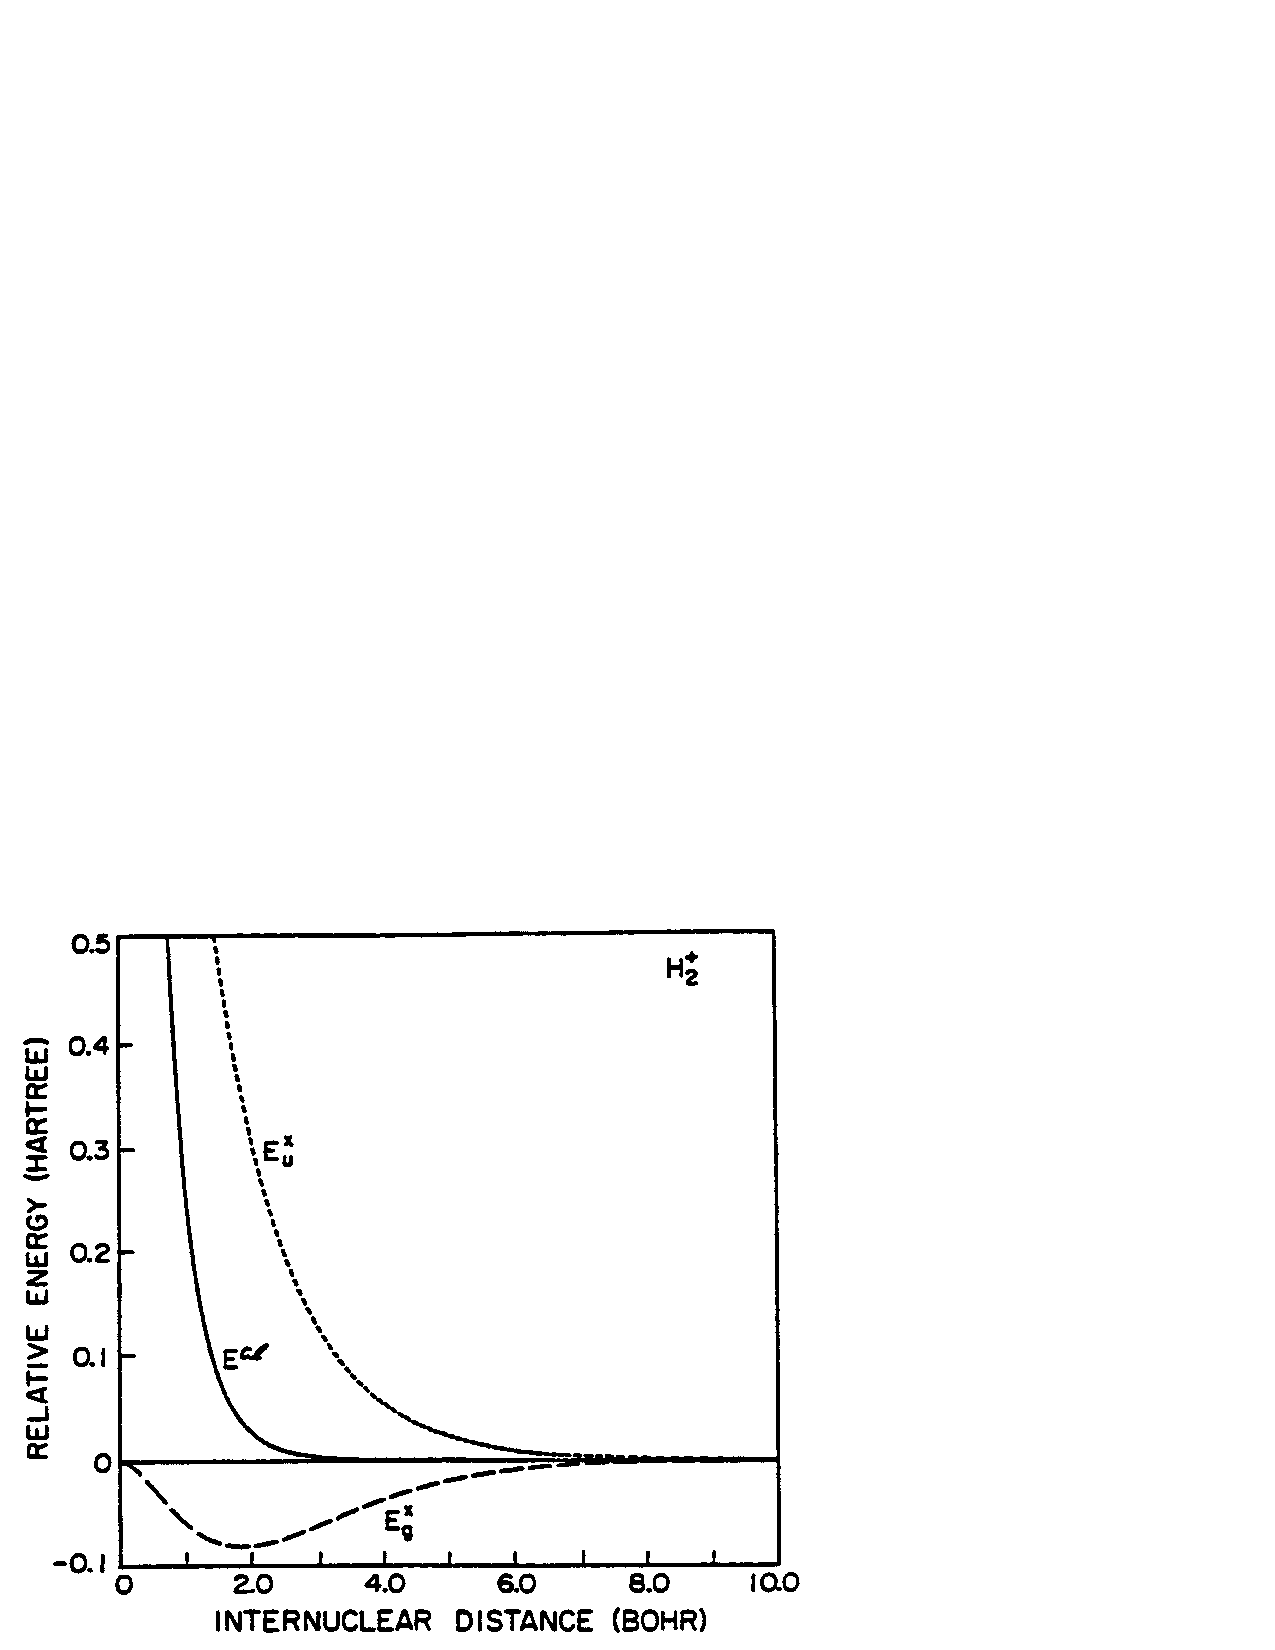
\includegraphics[scale=0.75]{fig2-13}
\caption{The classical energy and the exchange energies for the LCAO
  wave functions of H$_2^+$.}
\label{fig2-13}
\end{figure}

    
Consider first, the wavefunction for H$^+_2$ with no superimposition
of atomic orbitals, $\varphi^{cl} = \chi_{\ell}$.  We refer to this as
the classical wavefunction because it does not have interference
effects arising from superposition of atomic orbitals. The energy of
this wavefunction, $\epsilon^{cl}$, is nonbonding, as shown in Figure
\ref{fig2-13}.  Using equation (\ref{eqno2-7}), we obtain
\begin{equation}
\epsilon^{cl} = \langle \chi_{\ell} \vert H \vert \chi_{\ell}\rangle = 
\langle \chi_{\ell} \vert - {1 \over 2} \nabla^2 - {1 \over r_a} - 
{1 \over r_b} \vert \chi_{\ell} \rangle = \epsilon_{atom} + \langle 
\chi_{\ell} \vert - {1 \over r_b} \vert \chi_{\ell} \rangle,
\end{equation}
where
\begin{equation}
\epsilon_{atom} = \langle \chi_{\ell} \vert - {1 \over 2} \nabla^2 - 
{1 \over r_a} \vert \chi_{\ell} \rangle = - {1 \over 2} \left( {e^2 
\over a_0} \right).
\end{equation}
Thus,
\begin{equation}
\epsilon^{cl} + {1 \over R} = \epsilon_{atom} + \delta {\bar v}^{cl},
\end{equation}
where
\begin{equation}
\delta {\bar v}^{cl} = \left[\left\langle \chi^2_{\ell} \left( - {e^2 
\over r_b} \right)\right\rangle  + {e^2 \over r} \right]
\end{equation}
is repulsive.

\subsubsection{The Exchange Energy}
    
Now we consider the wavefunction $\varphi_g$ with energy
\begin{equation}
\epsilon_g = {\langle l + r \vert {\hat H} \vert l + r \rangle 
\over \langle l + r \vert l + r \rangle} = {\langle l \vert H \vert 
l + r \rangle \over \langle l \vert l + r \rangle}.
\end{equation}
Since
\begin{eqnarray*}
\langle l \vert {\hat H} \vert l + r \rangle &=& 
\langle l \vert {\hat H} \vert l + r \rangle +
\langle l \vert {\hat H} \vert r \rangle = \epsilon^{cl} +
\langle l \vert {\hat H} \vert r \rangle\cr
\langle l \vert l + r \rangle &=& \langle l \vert l \rangle + \langle 
l \vert r \rangle = 1 + S,\cr
\end{eqnarray*}
we obtain
\begin{equation}
\epsilon_g = {\epsilon^{cl} + \langle l | {\hat H} | r \rangle \over 
1 + S} = \epsilon^{cl} + {\langle l | {\hat H} | r \rangle - 
\epsilon^{cl} S \over 1 + S}
\end{equation}
hence
\begin{equation}
\epsilon_g = \epsilon^{cl} + {\tau \over 1+S},
\end{equation}
where
\begin{equation}
\tau = \langle l | {\hat H} | r \rangle - S \epsilon^{cl} = \left[ 
h_{lr} + S {1 \over R} \right] - S \left[ h_{ll} + {1 \over R} \right]
\end{equation}
or
\begin{equation}
\tau = h_{lr} - Sh_{ll}.
\label{eqno2-16}
\end{equation}
Similarly,
\begin{equation}
\epsilon_u = {\langle l - r | {\hat H} | l - r \rangle \over \langle 
l - r | l - r \rangle} = {\langle l | {\hat H} | l - r \rangle \over 
\langle l | l - r \rangle} = {\epsilon^{cl} - \langle l | {\hat H} | 
r \rangle \over 1 - S}
\end{equation}
or
\begin{equation}
\epsilon_u = \epsilon^{cl} + {\tau \over 1-S},
\end{equation}
where $\tau$ is again given by equation (\ref{eqno2-16}). Thus, the
interference resulting from superimposing the $\chi_\ell$ and $\chi_r$
wavefunctions can be viewed as corrections upon the classical energy,
\begin{equation}
\epsilon_g = \epsilon^{cl} + \epsilon_g^x
\end{equation}
\begin{equation}
\epsilon_u =  \epsilon^{cl} + \epsilon_u^x,
\end{equation}
where the correction terms
\begin{equation}
\epsilon_g^x = {\tau \over 1+S}
\label{eqno2-17a}
\end{equation}
\begin{equation}
\epsilon_u^x = {-\tau \over 1-S}
\label{eqno2-17b}
\end{equation}
are referred to as interference, exchange, or resonance terms. These
energies are shown in Figure \ref{fig2-12}, where we see that
$\epsilon_g^x$ favors bond formation, while $\epsilon^x_u$ opposes
bond formation.
    
The classical energy, as defined above, is the total energy of the
system if the wavefunction is forced to remain an atomic orbital as
$R$ is decreased. The exchange part of the energy is the change in the
energy due to the interference of $\chi_\ell$ and $\chi_r$, that is, due
to exchange of the electron between the left and right centers. As
shown in Figure \ref{fig2-12}, $\epsilon^{cl}$ is weakly antibonding,
and hence, bonding in the $g$ state of H$^+_2$ results from the
exchange energy $\epsilon^x_g$.  On the other hand, the exchange term
$\epsilon_u^x$ for the $u$ state is strongly repulsive, resulting in a
strongly antibonding potential curve.
    
These quantities $\epsilon_g^x$ and $\epsilon_u^x$ constitute a 
quantitative representation of
the effects discussed qualitatively in the first section. Thus, the 
decrease in kinetic energy for the $g$ states resulting from the 
decrease in the average gradient in the wavefunction
yields a large negative contribution to $\tau$. The increase in the 
potential energy for the $g$ state arising from the shift of charge 
from the nuclear to the bond region, yields a positive
contribution to $\tau$. The net result is a negative $\tau$, leading 
to a negative value for
\begin{equation}
\epsilon_g^x = {\tau \over (1+S)}
\end{equation}    
and a positive value for
\begin{equation}    
\epsilon_u^x = {- \tau \over (1-S)}.
\end{equation} 

\subsubsection{Comparison of $g$ and $u$ States}
    
For large $R$, where the overlap $S$ is nearly zero, we see that
equations (\ref{eqno2-17a})--(\ref{eqno2-17b}) lead to
\begin{equation}
\epsilon_g^x = \tau
\end{equation}
and
\begin{equation}
\epsilon_u^x = - \tau,
\end{equation}
so that the bonding in the $g$ state and the antibonding in the $u$ 
state are equal.
    
However, for small $R$ the $(1 + S)$ and $(1 - S)$ terms lead to 
asymmetry, where the antibonding state is several times more antibonding 
than the bonding state is bonding.  Thus, at $R = 2.5\ a_0 = 1.32$ \AA, 
we have $S = 0.4583$, and $\tau  = -0.1083(e^2 /a_0)$, leading to
\begin{equation}
\epsilon_g^x = - 0.0742 \left( {e^2 \over a_0} \right)
\end{equation}
\begin{equation}
\epsilon_u^x = + 0.20939 \left( {e^2 \over a_0} \right),
\end{equation}
whereas
\begin{equation}
\epsilon^{cl} = 0.00943 \left( {e^2 \over a_0} \right) .
\end{equation}

\medskip

\subsubsection{Analytic Results}

Explicit evaluation of the various quantities involved in the energy of
H$^+_2$ is carried out in Section \ref{appendix-a}, leading to
\begin{eqnarray*}
S &=& \left[ 1 + R + {1 \over 3} R^2 \right] e^{-R}\cr
\epsilon^{cl} &=& - {1 \over 2} + \left( 1 + {1 \over R} \right) 
e^{-2R},\cr
\end{eqnarray*}
and
\begin{eqnarray*}
\tau &=& - \left[ {2 \over 3} R - {1 \over R} \right] e^{-R} - \left( 
1 + {1 \over r} \right) \left( 1 + R + {1 \over 3} R^2 \right) 
e^{-3R}\cr
&\approx&  - \left[ {2 \over 3} R - {1 \over R} \right] e^{-R},\cr
\end{eqnarray*}
where terms of order $e^{-3R}$ are neglected. Thus, for large $R$
\begin{equation}
\tau \approx - {2 \over R} S.
\end{equation}
That is, the quantity $\tau$ dominating the bond in H$^+_2$ is 
proportional to the overlap between the orbitals. At large $R$, this 
leads to a bond strength of the form
\begin{equation}
\tau \approx - {2 \over 3} Re^{-R}.
\end{equation}
Thus, the bond energy decreases exponentially with internuclear distance.
    
This simple relation between bonding does not hold for small $R$.  We
saw, above, that $\tau$ is a minimum (most negative) at $R = 2\ a_0$,
and the total energy is also a minimum (bonding a maximum) around $R =
2\ a_0$. On the other hand, the overlap continues to increase as $R$
is decreased until $S = 1$ at $R = 0$.

\subsubsection{Contragradience}
    
The above discussions indicate that the interference or exchange part of the
kinetic energy dominates the bonding in H$^+_2$. This term is dominated by
\begin{equation}
t^x = {1 \over 2} \left[ \langle \left( \nabla \chi_\ell \right) + 
\left( \nabla \chi_r \right) \rangle - S \langle \left( \nabla 
\chi_\ell \right)^2 \rangle \right],
\end{equation}
which is large and negative in between the atoms. The region of space leading
to negative $\nabla \chi_\ell \cdot \nabla \chi_r$, and hence, dominating the 
bond, is indicated for H$_2$ in Figure \ref{fig2-14}.

\begin{figure}
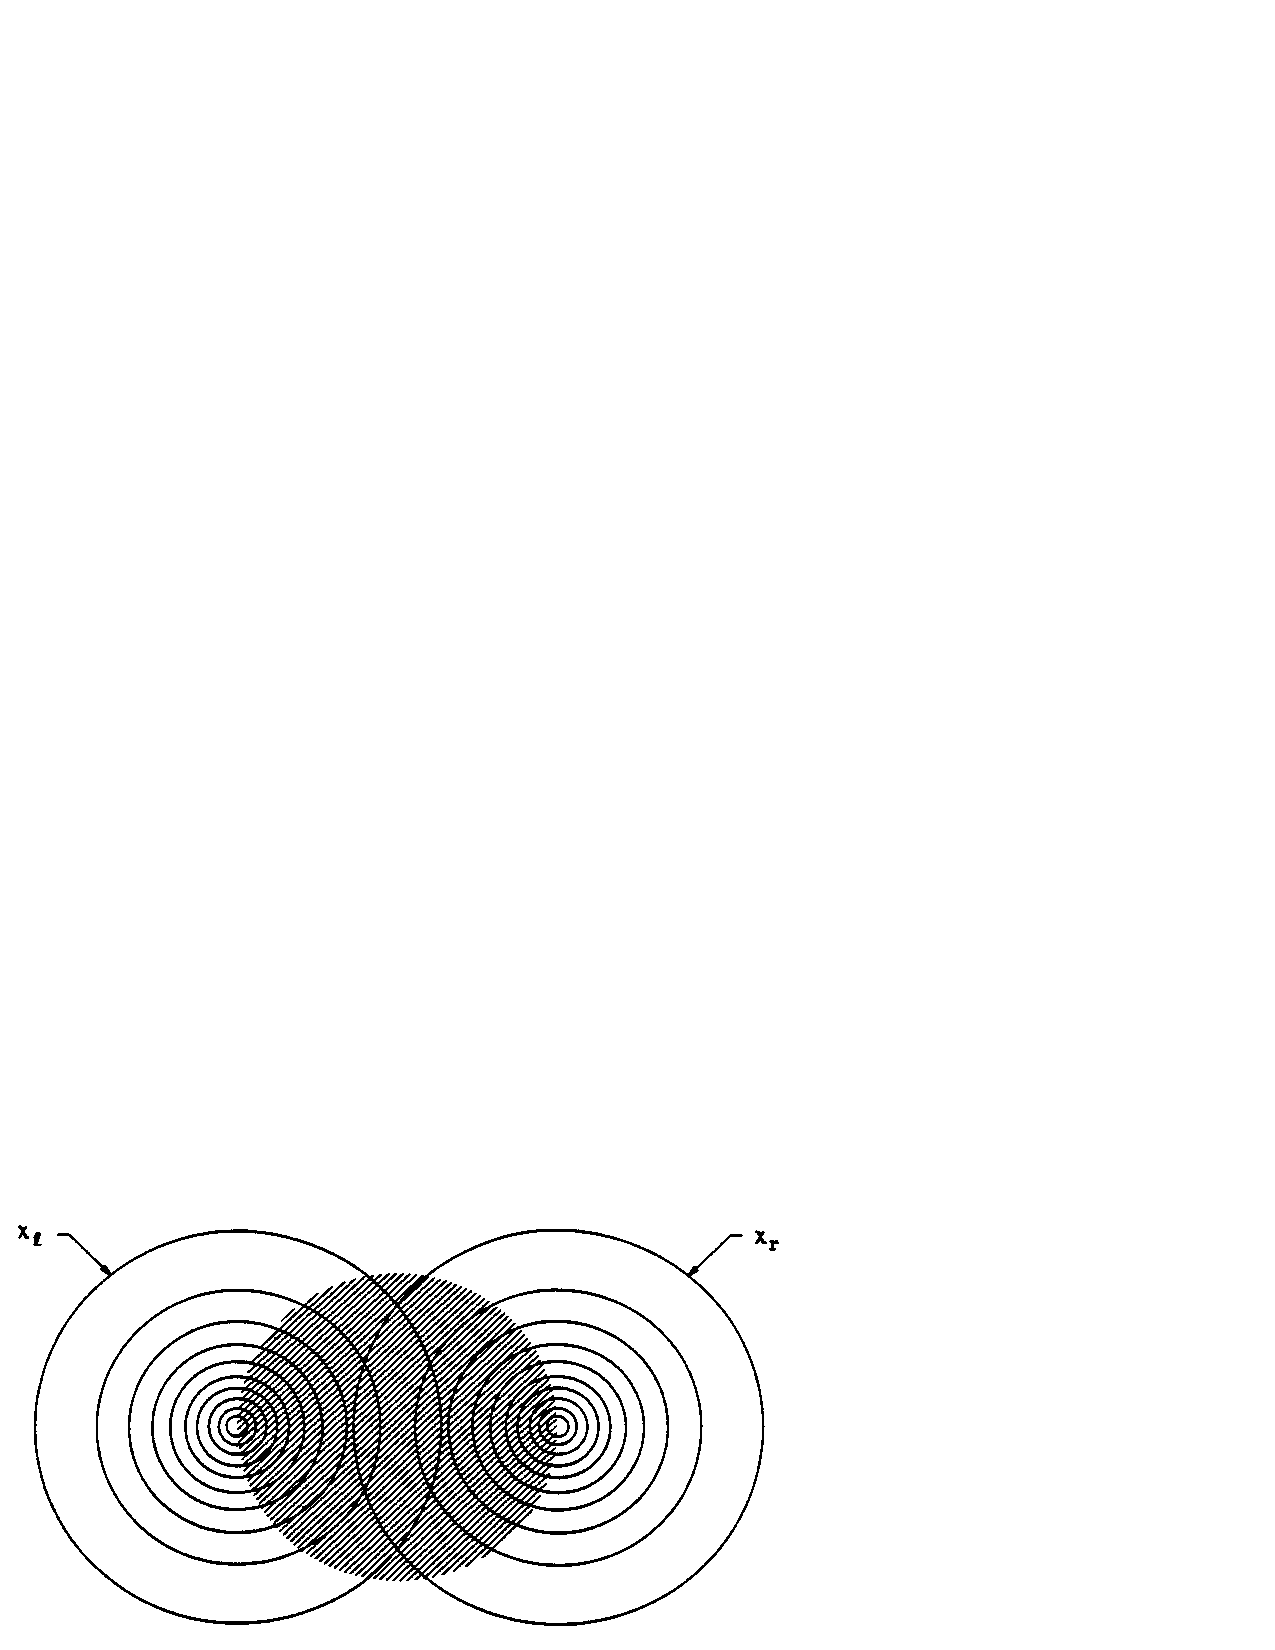
\includegraphics[scale=0.75]{fig2-14}
\caption{Contour plots of two hydrogen atomic orbitals for $R = 2 a_0$
(contour increment 0.05 a.u.). The shaded region leads to negative
  values of $\nabla\chi_\ell\cdot\nabla\chi_r$ and hence to a large
  contragradience. As a result, this region dominates the bonding.}
\label{fig2-14}
\end{figure}
    
\subsubsection{Historical Development}
    
\begin{figure}
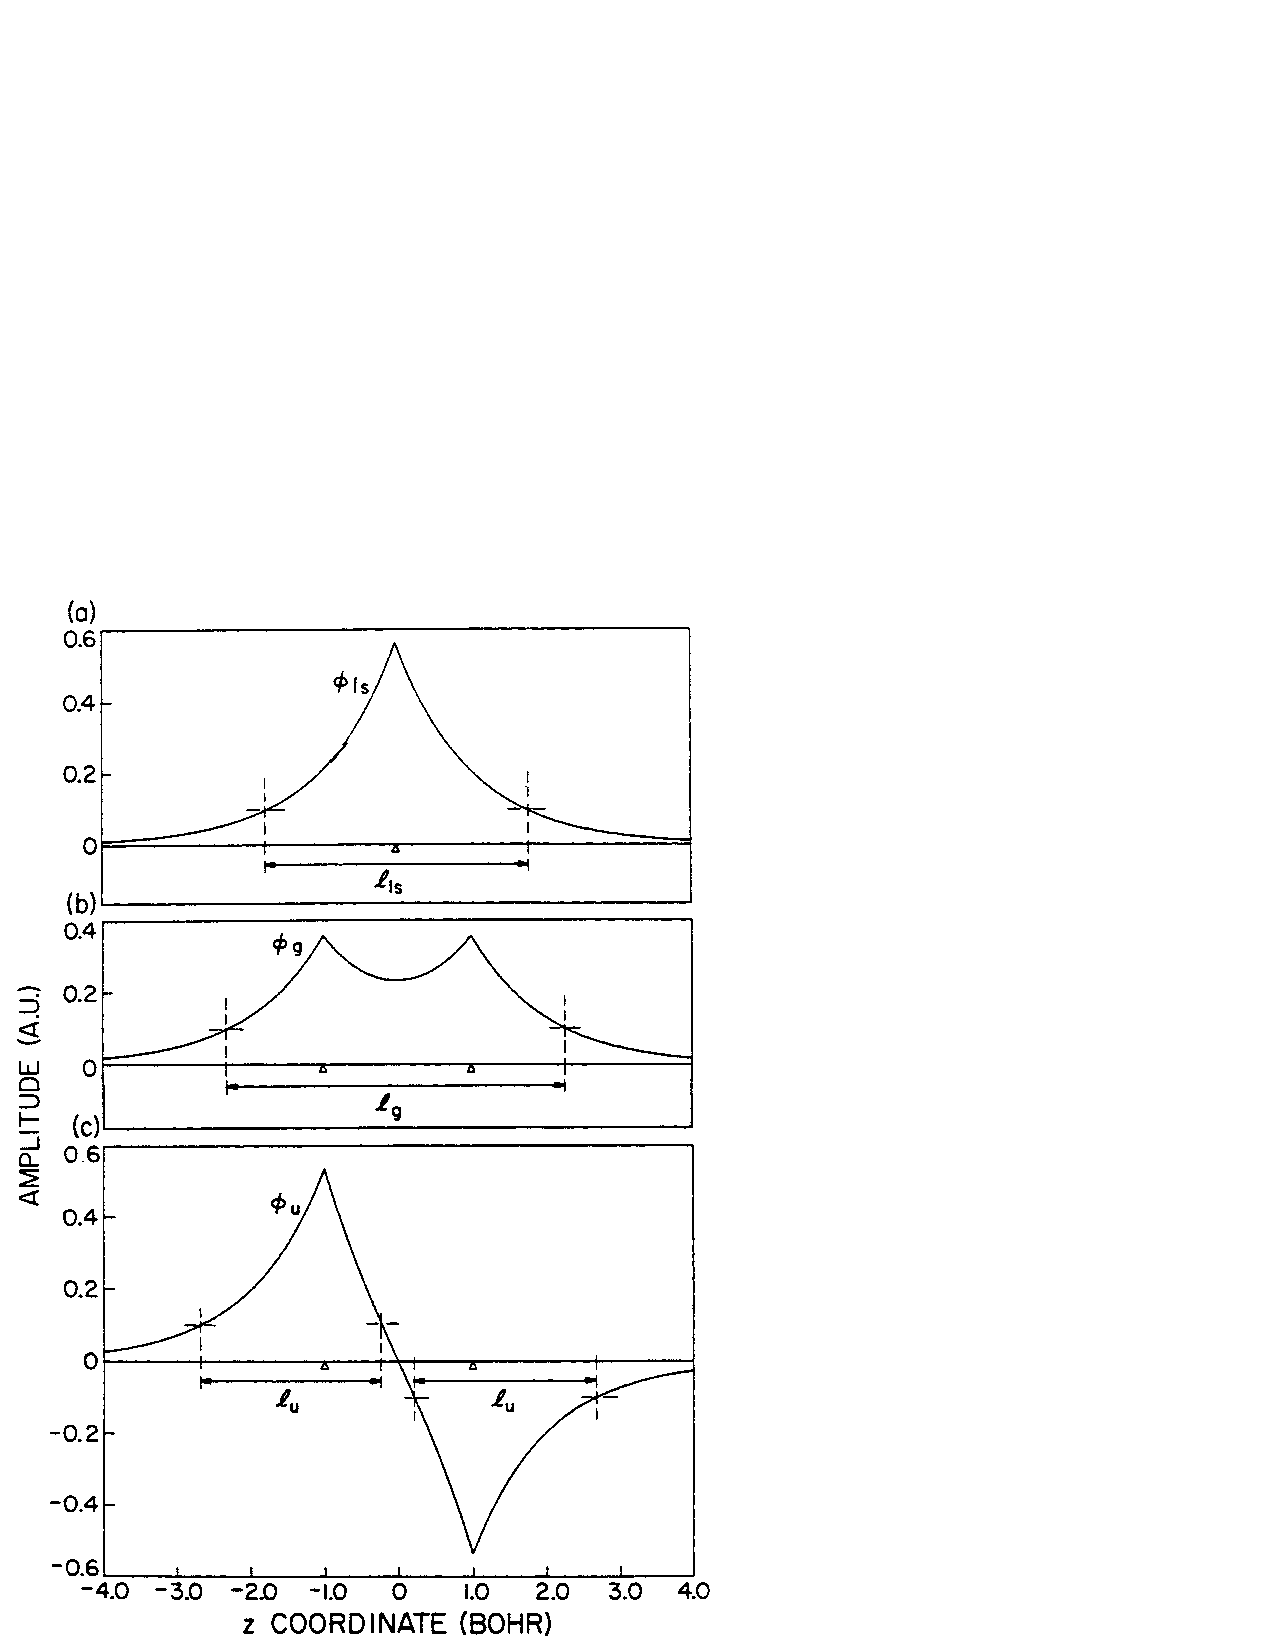
\includegraphics[scale=0.75]{fig2-15}
\caption{Illustration of the differences in the effective size of the
  box for the electron in the hydrogen atom and in the $g$ and $u$
  states of H$_2^+$.}
\label{fig2-15}
\end{figure}

H. Hellmann \cite{hellmann},after escaping from Hitler Germany into
Russia around 1934, and before suddenly vanishing into Stalin Russia
around 1937, was the first to suggest that bonding arises essentially
from a decrease in kinetic energy. He suggested that the bond in
H$^+_2$ results because the electron is allowed to delocalize over the
region spanning two protons rather than just one. Using the
uncertainty principle, he reasoned that a bigger 'box' for the
electron leads to a lower kinetic energy. Essentially, the idea is as
illustrated in Figure \ref{fig2-15}, where we see that for the
$\varphi_g$ state, the electron is distributed over a larger volume in
H$^+_2$ than in $H$ atom.  From the study of a particle-in-a-box, we
know that the kinetic energy decreases as the box is made
larger. Hence, because of a decrease in kinetic energy, the
$\varphi_g$ state is expected to be stablized with respect to $H$
atoms.
    
On the other hand, since the $\varphi_u$ state has a node in the middle, 
the energy is just the same as if we had put the electron in either of two 
boxes, each of which is smaller than for $H$ atom. This leads to an increase 
in the kinetic energy.
    
Hellmann presented only very simple qualitative ideas and his view of
bonding was largely ignored until K. Ruedenberg \cite{rudenberg}
provided a more quantitative framework showing, for specific cases,
that interference terms resulting from the superposition of amplitude
leads to a significant decrease in the kinetic energy. Indeed, most
workers before Ruedenberg, argued that the bonding results from
electrostatic interactions arising from increasing the density in the
bond region. The development in this chapter is derived from a series
of papers by Wilson and Goddard \cite{wilson-goddard1,
wilson-goddard2}. Other, somewhat related viewpoints, have also been
proposed by Feinberg and Ruedenberg \cite{feinberg-rudenberg},
Feinberg, Ruedenberg and Mebler \cite{feinberg-rudenberg-mebler}, and
Bader and Baudraut \cite{bader-baudraut}.

\section{The Molecular Orbital Description of H$_2$}
    
We will now add a second electron to H$^+_2$ to obtain the H$_2$ molecule.
The simplest wavefunction for H$_2$ is to start with an electron in the 
best molecular orbital of H$^+_2$, and to place a second electron in 
this $\varphi_g$ orbital. This leads
to the molecular orbital (MO) wavefunction for H$_2$,
\begin{equation}
\Phi^{MO}_{gg} \left( {\bf r}_1 , {\bf r}_2 \right) = \varphi_g ( 
{\bf r}_1 ) \varphi_g ( {\bf r}_2)
\label{eqno2-18}
\end{equation}
where
\begin{equation}
\varphi_g = {\left( \chi_\ell + \chi_r \right) \over D_g},
\label{eqno2-19a}
\end{equation}
and
\begin{equation}
D_g = \sqrt{2(1+S)}.
\label{eqno2-19b}
\end{equation}
With two electrons, the total wavefunction $\Phi ( {\bf r}_1 , {\bf
r}_2)$ must specify the probability amplitude for electron 1 to have
each possible value of its three coordinates ($x_1$, $y_1$, and $z_1$,
symbolized collectively as ${\bf r}_1$), and for electron 2 to have
each possible value of its three coordinates ($x_2$, $y_2$, and $z_2$,
symbolized collectively as ${\bf r}_2$). Thus, the wavefunction must be
specified for all six simultaneous components of ${\bf r}_1$ and ${\bf
r}_2$ as in equation (\ref{eqno2-18}).
    
First we will examine the meaning of the wavefunction
(\ref{eqno2-18}). The total probability for electron 1 to be at some
position ${\bf r}_1$, while electron 2 is simultaneously at some
position ${\bf r}_2$ is
\begin{equation}
P ( {\bf r}_1 , {\bf r}_2 ) = \vert \Phi^{MO} ( {\bf r}_1 , {\bf 
r}_2 ) \vert^2 = \vert \varphi_g ( {\bf r}_1 ) \vert^2 \vert \varphi_g 
( {\bf r}_2 )  \vert^2 = P_g ( {\bf r}_1 ) P_g ( {\bf r}_2 ) .
\end{equation}
This is just the product of the independent, probabilities for
electron 1 to be at position ${\bf r}_1$, and electron 2 to be at
position ${\bf r}_2$. Thus, the probability distribution for electron
1 is independent of electron 2. (Consider the analogous case of a red
die, electron 1, and a green die, electron 2. The probability of
rolling a red 3 is 1/6 and the probability of rolling a green 5 is 1/6
so that the total probability of getting both a red 3 and a green 5 is
1/6 $\times$ 1/6 equal to 1/36. The dice are independent so that the
probabilities multiply.)  Summarizing, a product wavefunction as in
equation (\ref{eqno2-18}) implies that the electrons move
independently of each other (no correlations in their motions).
    
In addition to using the $\varphi_g$ molecular orbital, as in
equations (\ref{eqno2-19a})--(\ref{eqno2-19b}), we can construct
wavefunctions of H$_2$ using the $\varphi_u$ molecular orbital,
\begin{equation}
\varphi_u = { \left( \chi_\ell - \chi_r \right) \over \sqrt{2(1-S)}}.
\end{equation}
This leads to wavefunctions of the form
\begin{equation}
\Phi_{ug} ( 1 , 2 ) = \varphi_u ( 1 ) \varphi_g ( 2 ) ,
\label{eqno2-20}
\end{equation}
\begin{equation}
\Phi_{gu} ( 1 , 2 ) = \varphi_g ( 1 ) \varphi_u ( 2 ) ,
\label{eqno2-21}
\end{equation}
\begin{equation}
\Phi_{uu} ( 1 , 2 ) = \varphi_u ( 1 ) \varphi_u ( 2 ).
\label{eqno2-22}
\end{equation}
Since the $\varphi_u$ orbital is antibonding, the above wavefunctions
of H$_2$ lead to much higher energies than equation (\ref{eqno2-18}),
except at large $R$, and we expect an energy level diagram as in
Figure \ref{fig2-16}.

\begin{figure}
\begin{center}
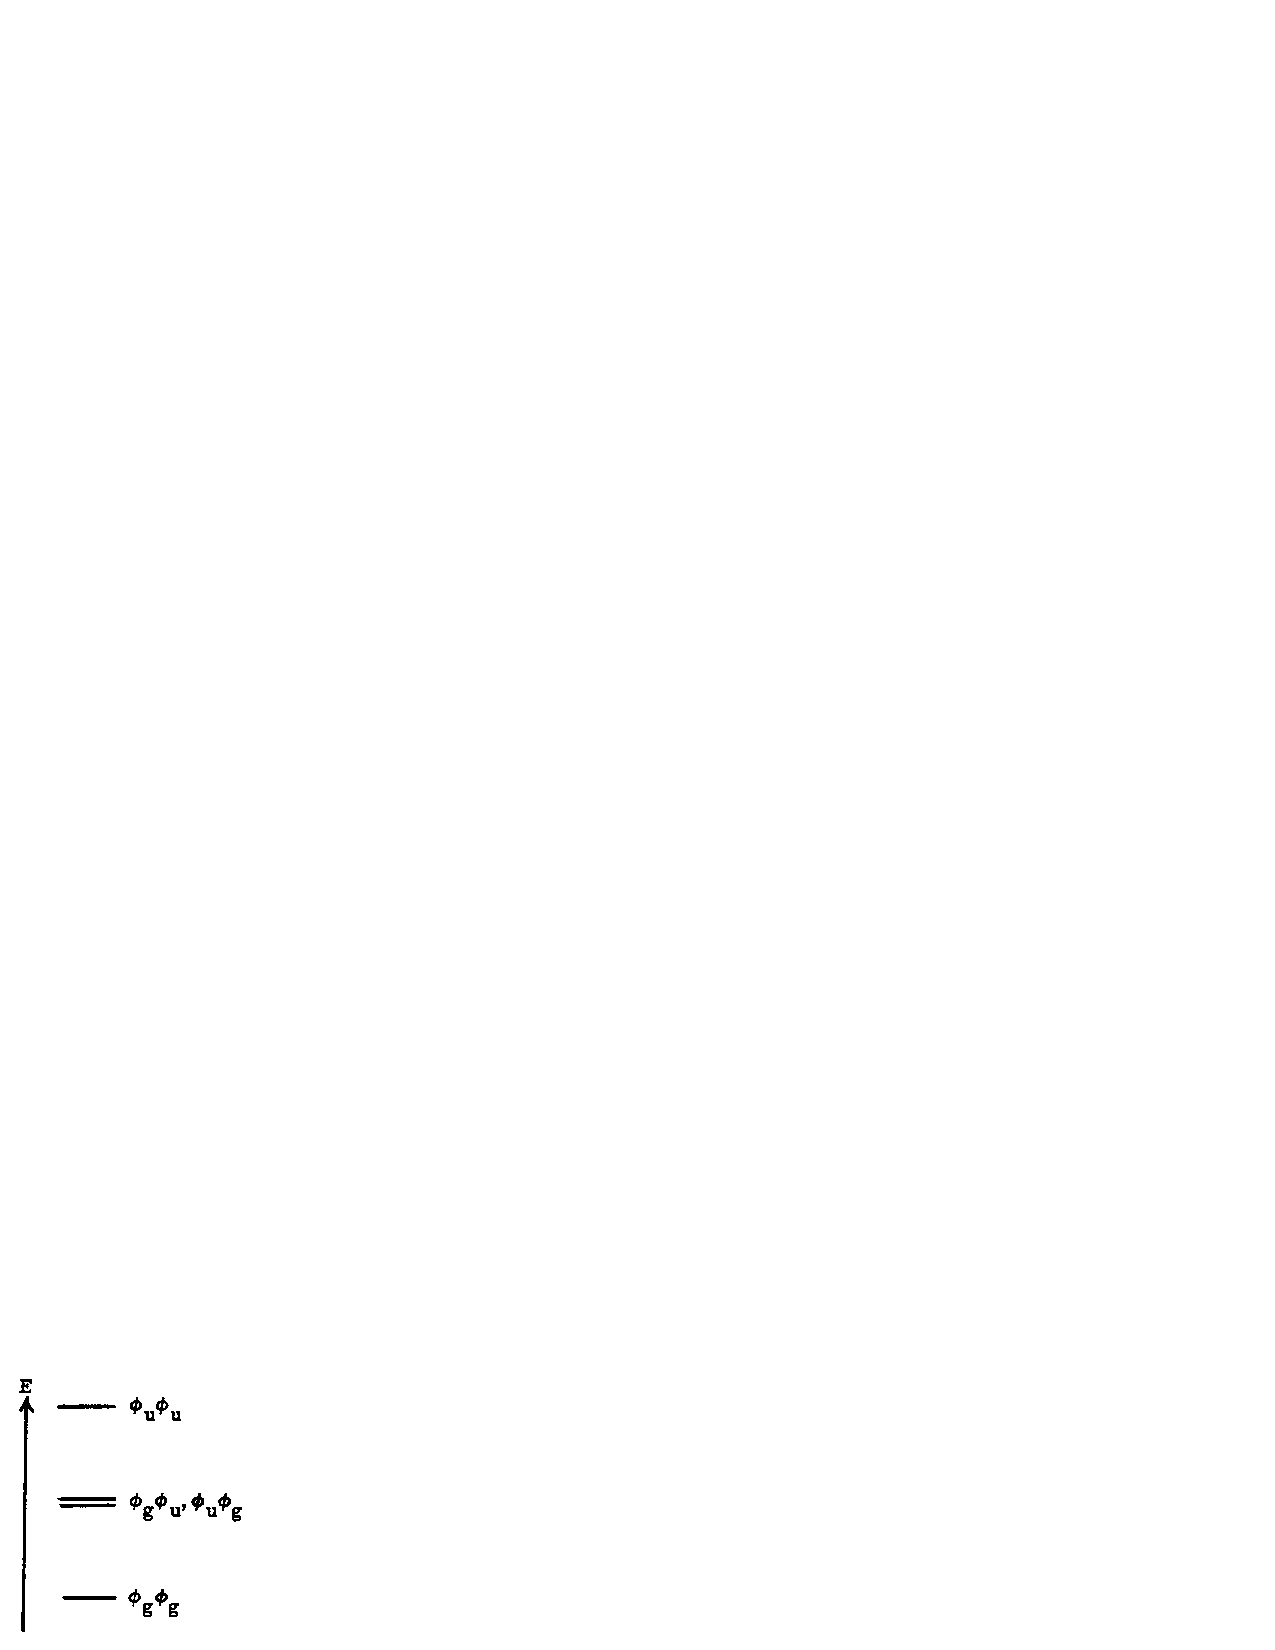
\includegraphics[scale=0.75]{fig2-16}
\end{center}
\caption{Simple energy diagram for MO wave functions of H$_2$.}
\label{fig2-16}
\end{figure}

\subsection{Energies}
    
\begin{figure}
\begin{center}
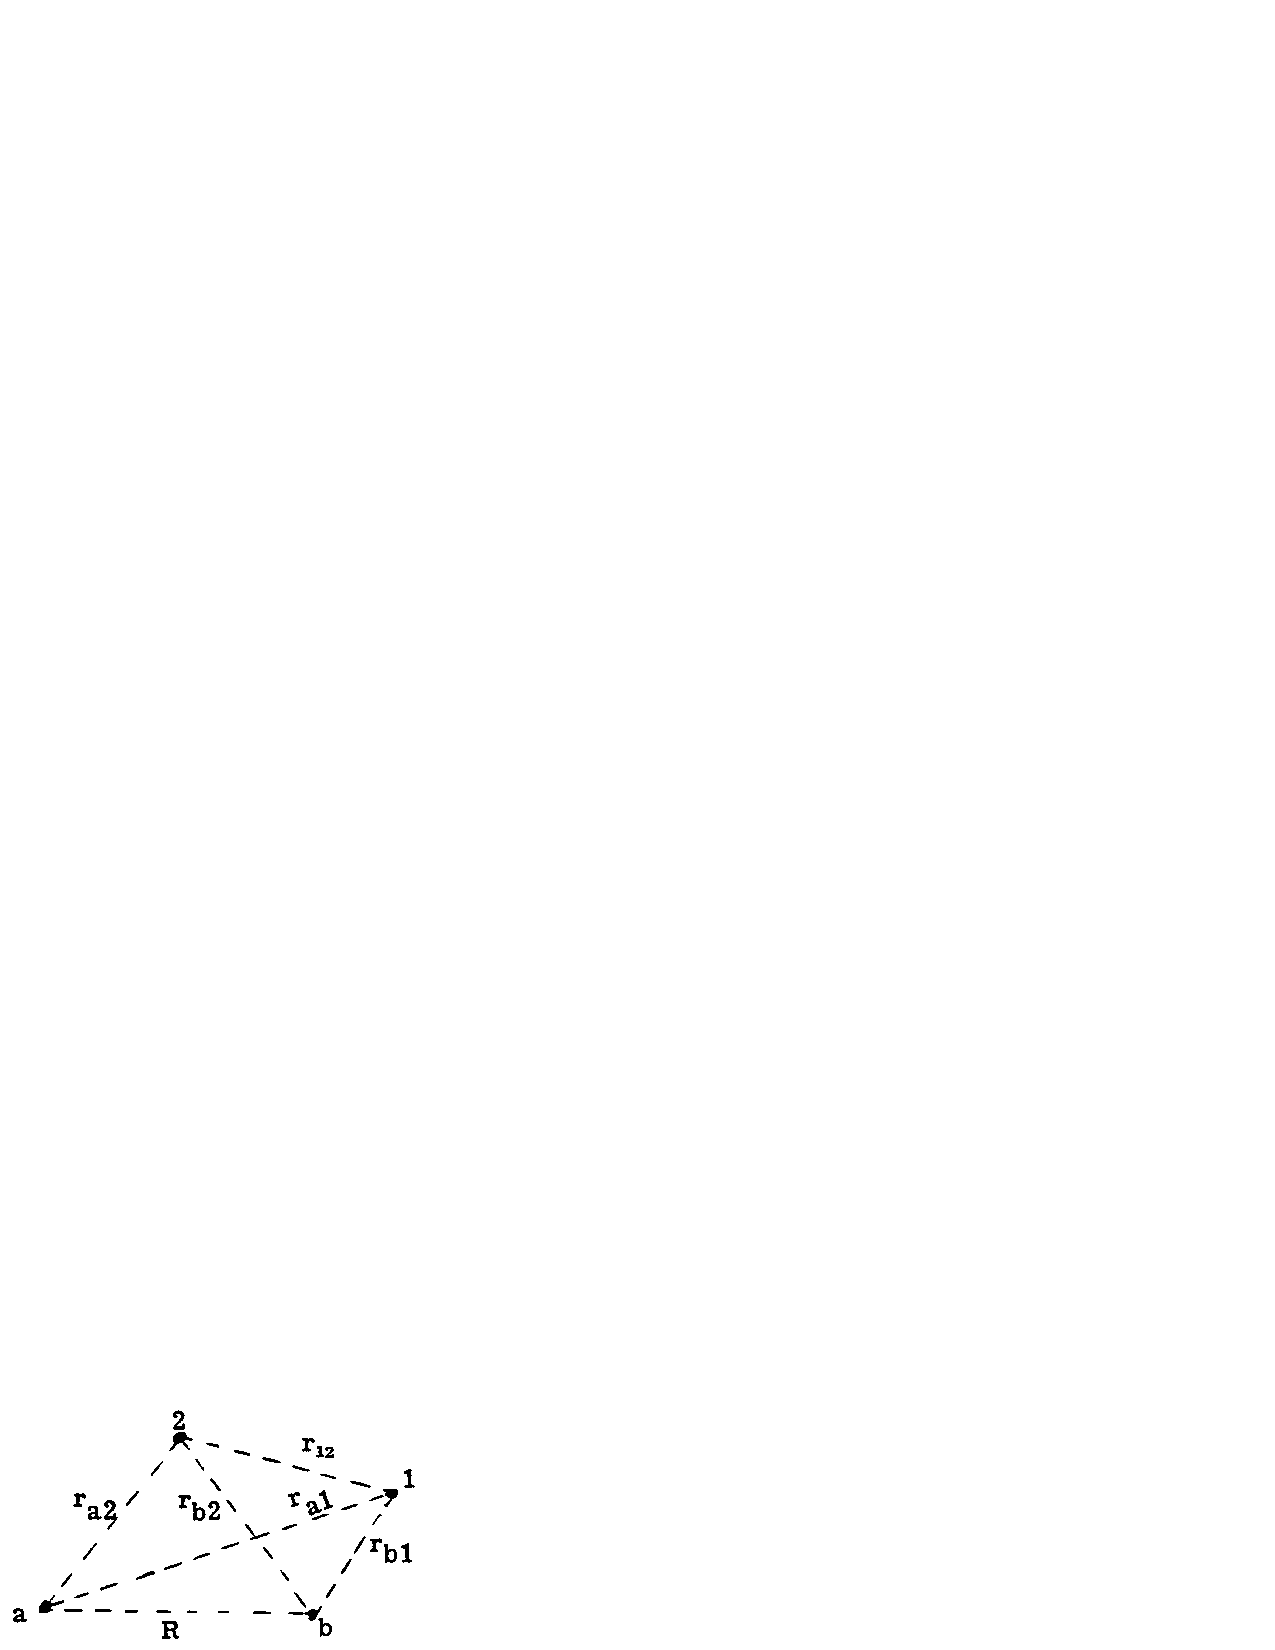
\includegraphics[scale=0.75]{fig2-17}
\end{center}
\caption{Coordinates for H$_2$.}
\label{fig2-17}
\end{figure}
    
For H$_2$, we use the coordinate system of Figure \ref{fig2-17}.
Using the same conventions and assumptions as for H$^+_2$ leads to the
Hamiltonian
\begin{equation}
{\hat H} \left( \mathrm{H}_2 \right) = h ( 1 ) + h ( 2 ) + {1 \over
r_{12}} + {1 \over R},
\end{equation}
where $1/r_{12}$ is the Coulomb interaction between the two electrons, and 
where
\begin{equation}
h ( i ) = - {1 \over 2} \nabla^2_i - {1 \over r_{ai}} - {1 \over 
r_{bi}}
\end{equation}
contains all terms depending only upon the coordinates of electron $i$.

Consider now the energy of a product wavefunction
\begin{equation}
\Phi_{ab} ( 1 , 2 ) = \varphi_a ( 1 ) \varphi_b ( 2 )
\end{equation}
and note that many two-electron integrals factor into products of 
one-electron integrals, e.g.,
\begin{eqnarray}
\langle \Phi_{ab} ( 1 , 2 ) | h ( 2 ) | \Phi_{ab} ( 1 , 2 ) 
\rangle &=& \int \int d^2 r_1 d^3 r_2 \varphi^*_a ( 1 ) \varphi^*_b ( 
2 ) h ( 2 ) \varphi_a ( 1 ) \varphi_b ( 2 )\cr
&=& \left[ \int d^3 r_1 \varphi^*_a ( 1 ) \varphi_a ( 1 ) \right] 
\left[ \int d^3 r_2 \varphi^*_b ( 2 ) h ( 2 ) \varphi_b ( 2 ) 
\right]\cr
&=& \langle \varphi_a | \varphi_a \rangle \langle \varphi_b | h | 
\varphi_b \rangle\cr
&=& \langle \varphi_b | h | \varphi_b \rangle
\end{eqnarray}
since $\langle \varphi_a | \varphi_a \rangle = 1$.  Note that the 
$\langle ~~ \rangle$ notation implies integration over however many
electrons are in the wavefunctions. In order to simplify the energy 
expressions, we will define
\begin{equation}
h_{ij} = \langle \varphi_i | h | \varphi_j \rangle.
\end{equation}
  
The integral that does not fact is the one arising from the $1/r_{12}$ terms
in the Hamiltonian, which we will denote as
\begin{equation}
J_{ij} = \langle \Phi_{ij} ( 1 , 2 ) \vert {1 \over r_{12}} \vert 
\Phi_{ij} ( 1 , 2 ) \rangle = \int \int d^3 r_1 d^3 r_2 
{\varphi^*_i ( 1 ) \varphi_i ( 1 ) \varphi^*_j ( 2 ) \varphi_j ( 
2 ) \over r_{12}}.
\label{eqno2-23}
\end{equation}
Note that
\begin{equation}
\rho_i ( 1 ) = \varphi^*_i ( 1 ) \varphi_i ( 1 )
\end{equation}
is the probability density for finding the electron in orbital $i$ 
at a position ${\bf r}_1$, and
\begin{equation}
\rho_j ( 2 ) = \varphi^*_j ( 2 ) \varphi_j ( 2 )
\end{equation}
is the probability density for finding the electron in orbital $j$ at
position ${\bf r}_2$.  Thus, we can rewrite equation (\ref{eqno2-23})
as
\begin{equation}
J_{ij} = \int \int d^3 r_1 d^3 r_2 {\rho_i ( 1 ) \rho_j ( 2 ) \over 
r_{12}}.
\label{eqno2-24}
\end{equation}
But equation (\ref{eqno2-24}) is just the classical electrostatic
interaction energy (the Coulomb energy) between the two charge
distributions $\rho_i$ and $\rho_j$. Thus, we refer to $J_{ij}$ as the
\emph{Coulomb integral} between orbitals $\varphi_i$ and
$\varphi_j$. This term cannot be factored into a product of
one-electron terms because of the
\begin{equation}
r_{12} = \sqrt{( x_1 - x_2 )^2 + (y_1 - y_2 )^2 + ( z_1 - z_2 )^2}
\end{equation}
term.

Since $\rho_i$, $\rho_j$, and $1/r_{ij}$ are always positive, we see 
that the Coulomb integral is always positive $J_{ij} \geq 0$. Using the 
above results, we can write
\begin{equation}
E_{gg} = 2 h_{gg} + J_{gg} + {1 \over R}
\label{eqno2-25}
\end{equation}
\begin{equation}
E_{gu} = h_{uu} + h_{gg} + J_{gu} + {1 \over R}
\label{eqno2-26}
\end{equation}
\begin{equation}
E_{ug} = E_{gu}
\end{equation}
\begin{equation}
E_{uu}  = 2 h_{uu} + J_{uu} + {1 \over R}.
\end{equation}
The molecular orbital states are ordered as in Figure
\ref{fig2-16}. Note there that the Coulomb interactions are not
negligible, but nonetheless, overall ordering of states can be
predicted solely from considering the one-electron terms.

\subsection{Symmetries}

Before proceeding further in the discussion of H$_2$, we will examine
how symmetry can help us in sorting out the states.

\subsubsection{Inversion}
    
\begin{figure}
\begin{center}
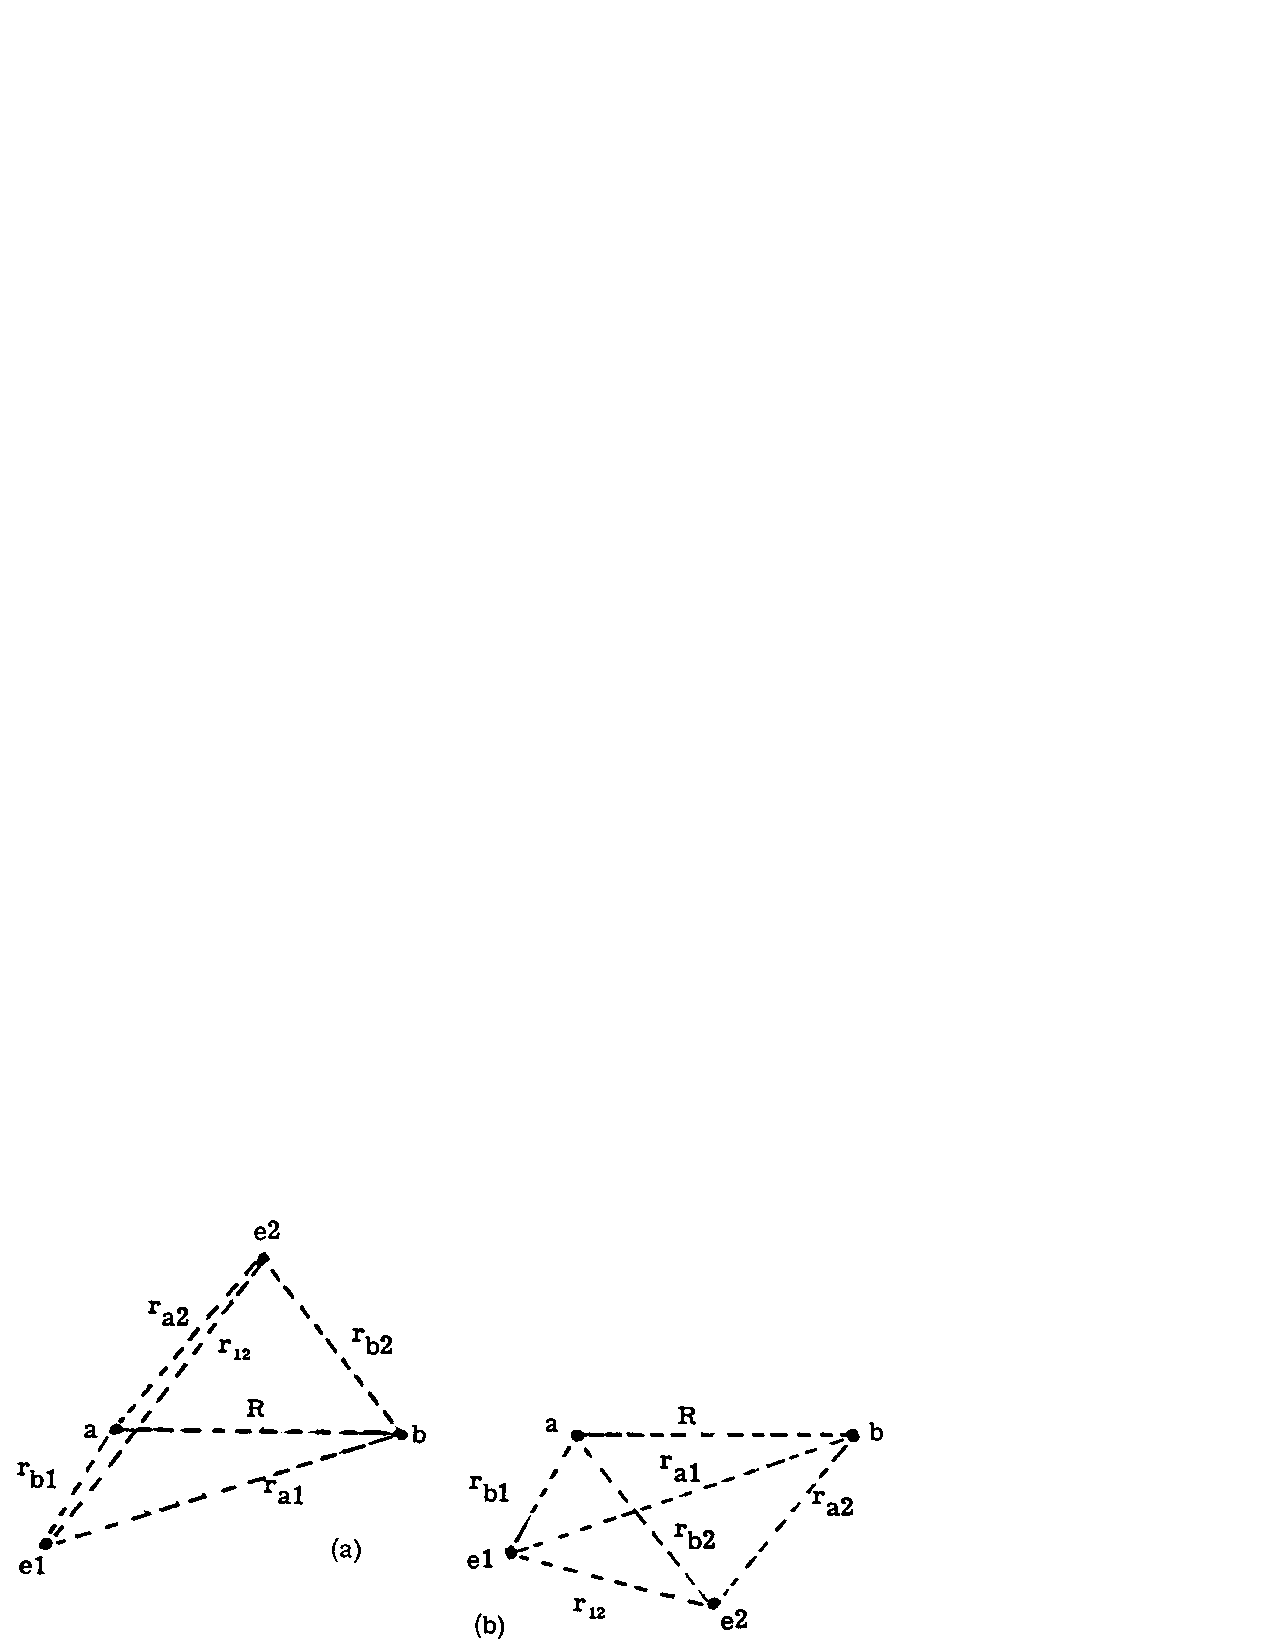
\includegraphics[scale=0.75]{fig2-18}
\end{center}
\caption{}
\label{fig2-18}
\end{figure}

Starting with the configuration of particles in Figure \ref{fig2-17}
and inverting the coordinates of electron 1, leads to Figure
\ref{fig2-18}(a), with electron 1 at a distance of $r_{b1}$ from the
nucleus $a$, and $r_{a1}$ from $b$.  Recall that the center of
inversion is the bond midpoint. Just as for H$^+_2$, this does not
change the nuclear attraction terms if the nuclei have identical
charges.  Even so, the total potential energy is changed since the
distance between electrons 1 and 2 is changed. Thus, in order to
preserve the same potential energy, we must simultaneously invert the
coordinates of both electrons, leading to Figure
\ref{fig2-18}(b). Thus, we define the inversion operator, ${\hat I}$,
for H$_2$ as $x_1 \rightarrow - x_1$, $y_1 \rightarrow - y_1$, $z_1
\rightarrow - z_1$ and $x_2 \rightarrow - x_2$, $y_2 \rightarrow -
y_2$, and $z_2 \rightarrow - z_2$ or $r_1 \rightarrow - r_1$ and $r_2
\rightarrow -r_2$, and the total Hamiltonian is invariant under this
inversion,
\begin{equation}
{\hat I} {\hat H} ( {\bf r}_1 , {\bf r}_2 ) = {\hat H} ( - {\bf 
r}_1 , - {\bf r}_2 ) = {\hat H} ( {\bf r}_1 , {\bf r}_2 ).
\label{eqno2-27}
\end{equation}
The exact wavefunction for H$_2$ is obtained by solving
\begin{equation}
{\hat H} ( 1 , 2 ) \Phi ( 1 , 2 ) = E \Phi ( 1 , 2 )
\label{eqno2-28}
\end{equation}
do not panic, we will not try this yet. Since ${\hat H}(1, 2)$ is
invariant under the inversion ${\hat I}$ (\ref{eqno2-27}), we find
that (\ref{eqno2-28}) implies
\begin{equation}
{\hat H} ( I \Phi ) = E ( I \Phi )
\end{equation}
and hence, just as for H$^+_2$, the exact eigenstates of H$_2$ are 
either $g$ or $u$,
\begin{equation}
{\hat I} \Phi_g ( 1 , 2 ) = + \Phi_g ( 1 , 2 )
\end{equation}
\begin{equation}
{\hat I} \Phi_u ( 1 , 2 ) = - \Phi_u ( 1 , 2 ).
\end{equation}

Applying the ${\hat I}$ operator to the MO wavefunctions
(\ref{eqno2-18}), (\ref{eqno2-20}), (\ref{eqno2-21}), and
(\ref{eqno2-22}) leads to the conclusion that $\Phi_{gg}$ and
$\Phi_{uu}$ are $g$ states, and $\Phi_{gu}$ and $\Phi_{ug}$ are $u$
states. Since a $u$ wavefunction must always have a nodal plane,
somewhere we expect the ground state of H$_2$ to be $g$, just as
indicated by Figure \ref{fig2-16}.

\subsubsection{Permutational Symmetry}

The Hamiltonian for H$_2$ is unchanged if we renumber the electrons so 
that electron 1 becomes electron 2 and vice versa, that is,
\begin{equation}
{\hat H} ( 2 , 1 ) = {\hat H} ( 1 , 2 ).
\label{eqno2-29}
\end{equation}
To discuss such symmetries, we define the transposition operator
$\tau_{12}$ as ${\bf r}_1 \rightarrow {\bf r}_2$ and ${\bf r}_2
\rightarrow {\bf r}_1$.  Thus, starting with the exact wavefunction
(\ref{eqno2-28}), applying $\tau_{12}$ to both sides, and using
equation (\ref{eqno2-29}), we find that
\begin{equation}
{\hat H} \left( \tau_{12} \Phi \right) = E \left( \tau_{12} \Phi 
\right).
\end{equation}
Since $( \tau_{12})^2$ transposes the electrons twice, taking us back 
to the original starting point,
\begin{equation}
 (\tau_{12})^2 = \tau_{12} \tau_{12} = e
\end{equation}
(where $e$ signifies doing nothing, i.e., the unity or \emph{einheit},
German, operator) we can show, just as for inversion, that the exact
eigenstates have the behavior
\begin{equation}
\tau_{12} \Phi^s ( 1 , 2 ) = \Phi^s ( 2 , 1 ) = + \Phi^s ( 1 , 2 )
\end{equation}
\begin{equation}
\tau_{12} \Phi^a ( 1 , 2 ) = \Phi^a ( 2 , 1 ) = + \Phi^a ( 1 , 2 )
\end{equation}
under transposition. Examining the wavefunctions (\ref{eqno2-18}),
(\ref{eqno2-20}), (\ref{eqno2-21}), and (\ref{eqno2-22}), we see that
\begin{equation}
\tau_{12} \left[ \varphi_g ( 1 ) \varphi_g ( 2 ) \right] = \left[ 
\varphi_g ( 1 ) \varphi_g ( 2 ) \right]
\end{equation}    
is symmetric,
\begin{equation}
\tau_{12}  \left[ \varphi_g ( 1 ) \varphi_u ( 2 ) \right] = \left[ 
\varphi_u ( 1 ) \varphi_g ( 2 ) \right],
\end{equation}    
\begin{equation}
\tau_{12} \left[ \varphi_u ( 1 ) \varphi_g ( 2 ) \right] = \left[ 
\varphi_g ( 1 ) \varphi_u ( 2 ) \right],
\end{equation}       
have no symmetry, and
\begin{equation}
\tau_{12} \left[ \varphi_u ( 1 ) \varphi_u ( 2 ) \right] = \left[ 
\varphi_u ( 1 ) \varphi_u ( 2 ) \right],
\end{equation}
is symmetric. Thus, the $g$ states, $\Phi_{gg}$ and $\Phi_{uu}$,
have the proper permutational symmetry,
but the $u$ states, $\Phi_{gu}$ and $\Phi_{ug}$, do not. In the next 
section, we will fix up this problem with the $u$ states.

\subsubsection{The $u$ States}

Combining the $u$ wavefunctions as follows
\begin{equation}
{^3}\Phi_u = \left( \varphi_g \varphi_u - \varphi_u \varphi_g 
\right)
\label{eqno2-30}
\end{equation}
\begin{equation}
{^1}\Phi_u = \left( \varphi_g \varphi_u + \varphi_u \varphi_g 
\right)
\label{eqno2-31}
\end{equation}
leads to
\begin{equation}
\tau_{12} {^3}\Phi_u = \left( \varphi_u \varphi_g - \varphi_g \varphi_u 
\right) = - {^3}\Phi_u
\end{equation}
\begin{equation}
\tau_{12} {^1}\Phi_u = \left( \varphi_u \varphi_g - \varphi_g \varphi_u 
\right) = + ^1\Phi_u
\end{equation}
so that the combinations (\ref{eqno2-30}) and (\ref{eqno2-31}) have
proper permutational symmetry. The notation will become clear when we
discuss spin, in Chapter \ref{chap04}.
    
Now we must examine the physics behind the combinations
(\ref{eqno2-30}) and (\ref{eqno2-31}). Aside from mathematical
analyses, indicating that the wavefunctions \emph{should} have
permutational symmetry, we also want to determine \emph{why} one
combination is favored in terms of achieving a lower energy.
    
In order to carry out such an analysis, we will plot the two-electron
wavefunction for the case where both electrons 1 and 2 are along the
bond axis, $z$. In order to show the relative locations of both
electrons, we will let the $z$ coordinate of electron 1 be the
ordinate, $z_1$, and the $z$ coordinate of electron 2 be the abscissa,
$z_2$. This is indicated in Figure \ref{fig2-19}, where some special
points are included.

\begin{figure}
\begin{center}
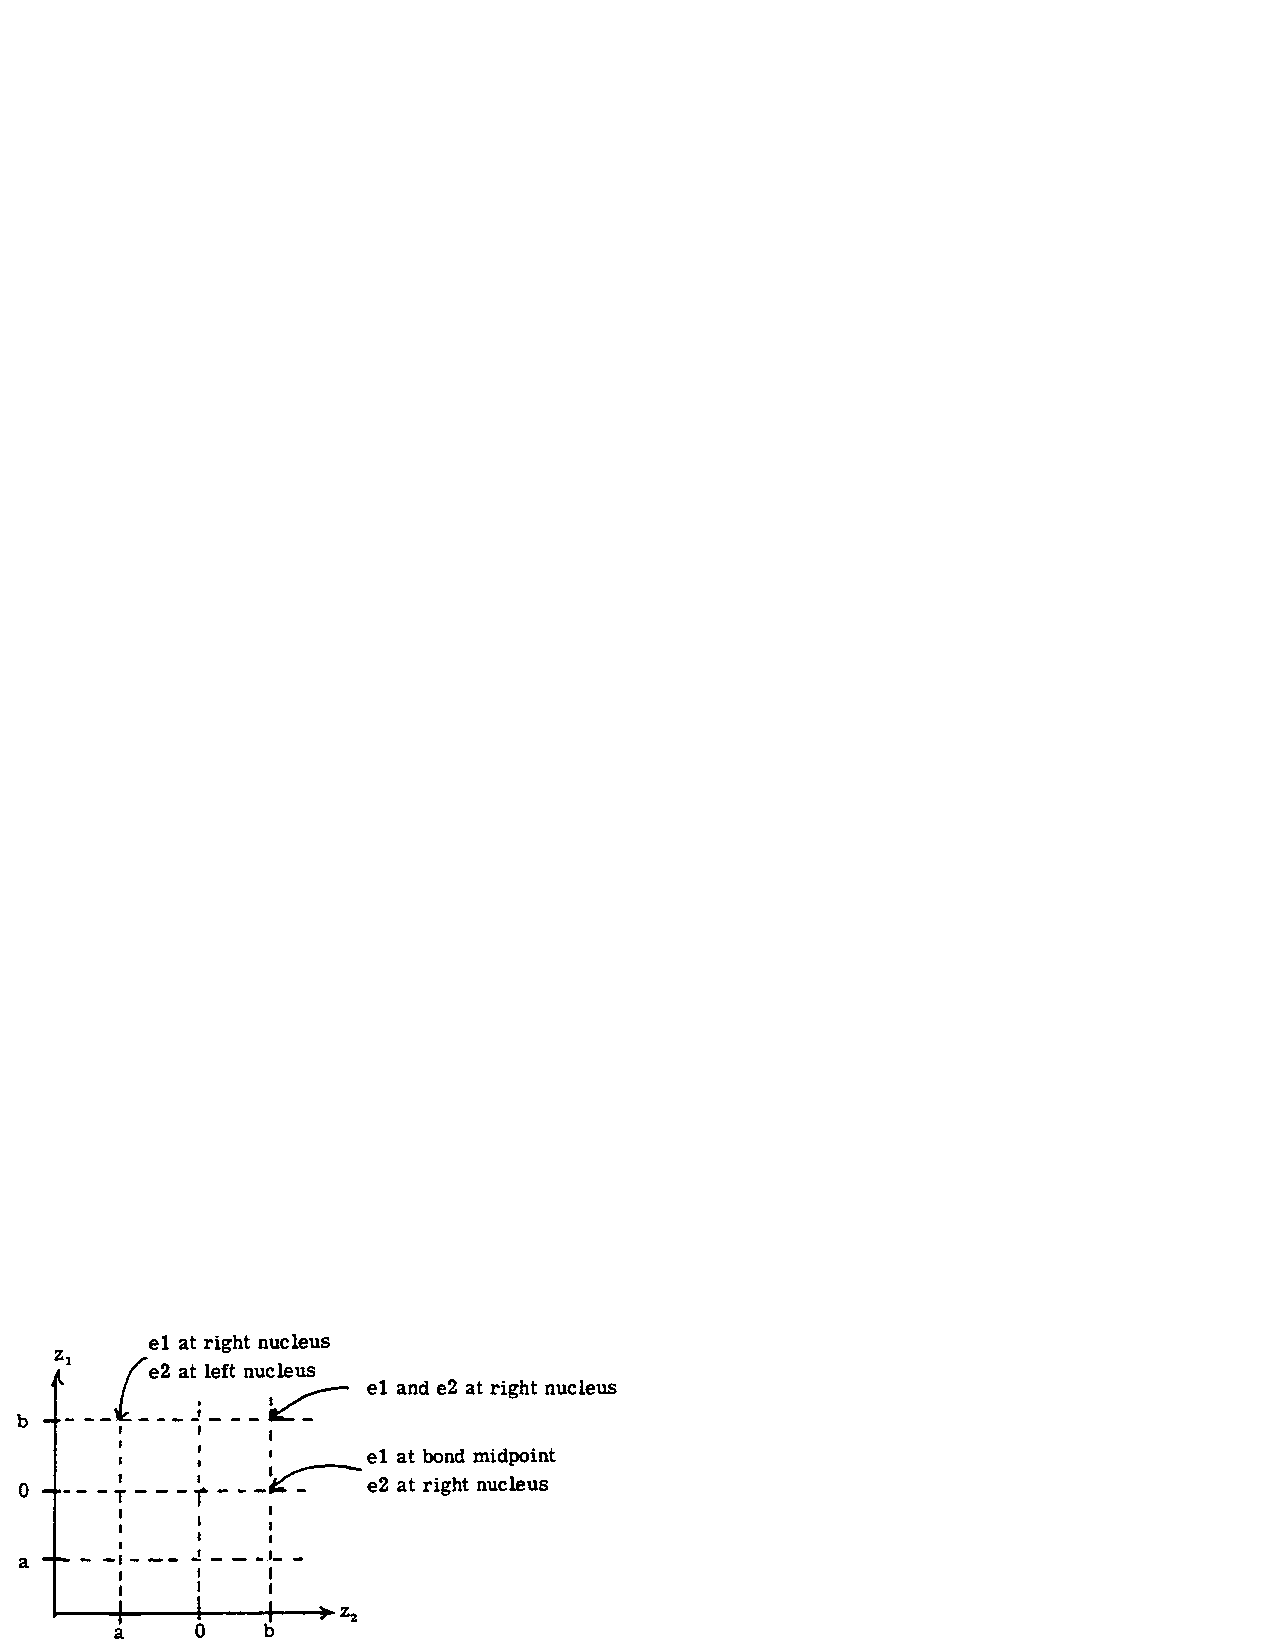
\includegraphics[scale=0.75]{fig2-19}
\end{center}
\caption{Coordinates showing simultaneous positions for $z_1$ and $Z_1$}
\label{fig2-19}
\end{figure}

\begin{figure}
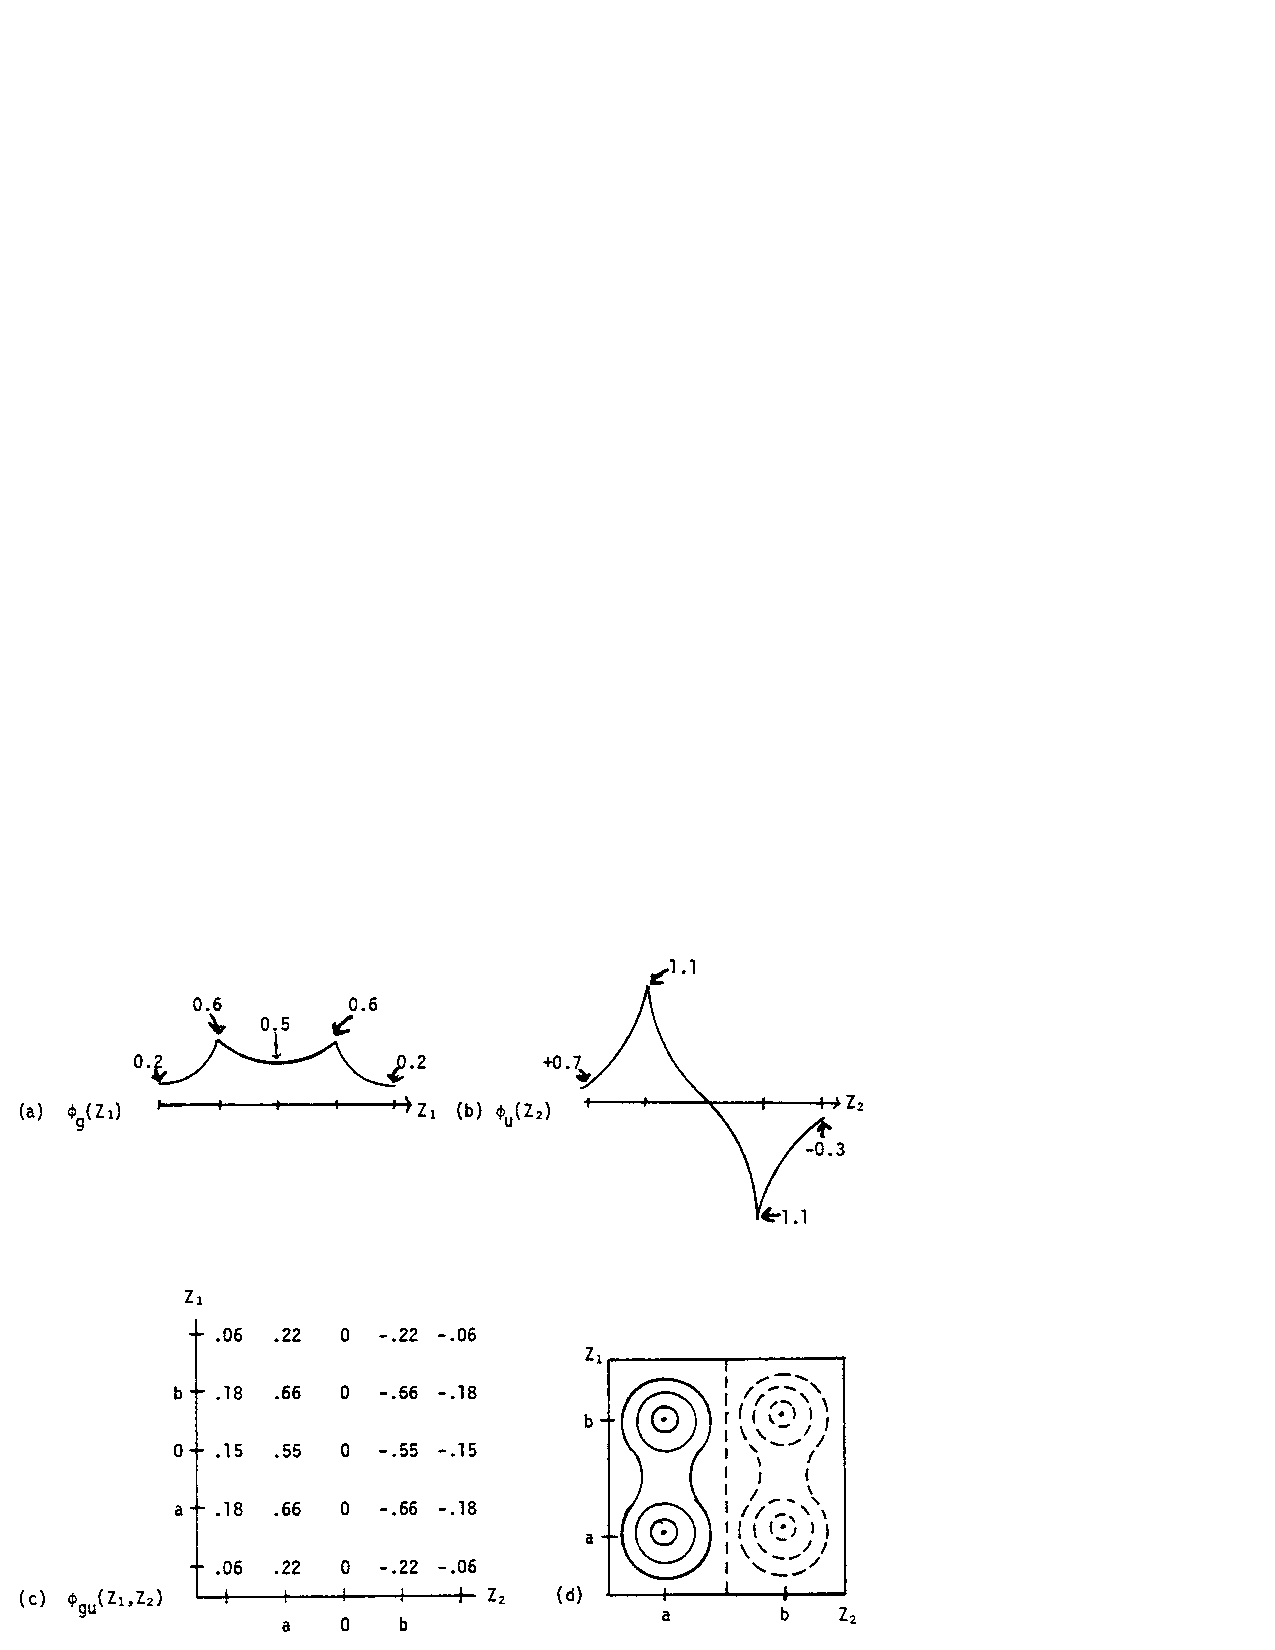
\includegraphics[scale=0.75]{fig2-20}
\caption{}
\label{fig2-20}
\end{figure}
    
Multiplying these orbitals leads to the wavefunction
$\Phi_{gu}(z_1,z_2)$ with amplitudes at various points, as given in
Figure \ref{fig2-20}(c). Rather than listing numbers as in Figure
\ref{fig2-20}(c), we will draw contours of equal amplitude as
indicated in Figure \ref{fig2-20}(d), where solid lines indicate
positive amplitude, dotted lines indicate negative amplitude, and long
dashes indicate zero amplitude. Here, one sees the maximum positive
amplitude occurs for $z_2 = b$ and $z_1 = a$ or $b$, while the
amplitude remains large or positive between the above two points. The
maximum negative amplitude occurs for $z_2 = b$ and $z_1 = a$ or $b$,
and remains large between the above two points. For $z_2 = 0$, the
total wavefunction is zero, independent of $z_1$. The reader should
practice constructing Figure \ref{fig2-20}(d) directly from Figures
\ref{fig2-20}(a) and \ref{fig2-20}(b), without going through Figure
\ref{fig2-20}(c).
    
\begin{figure}
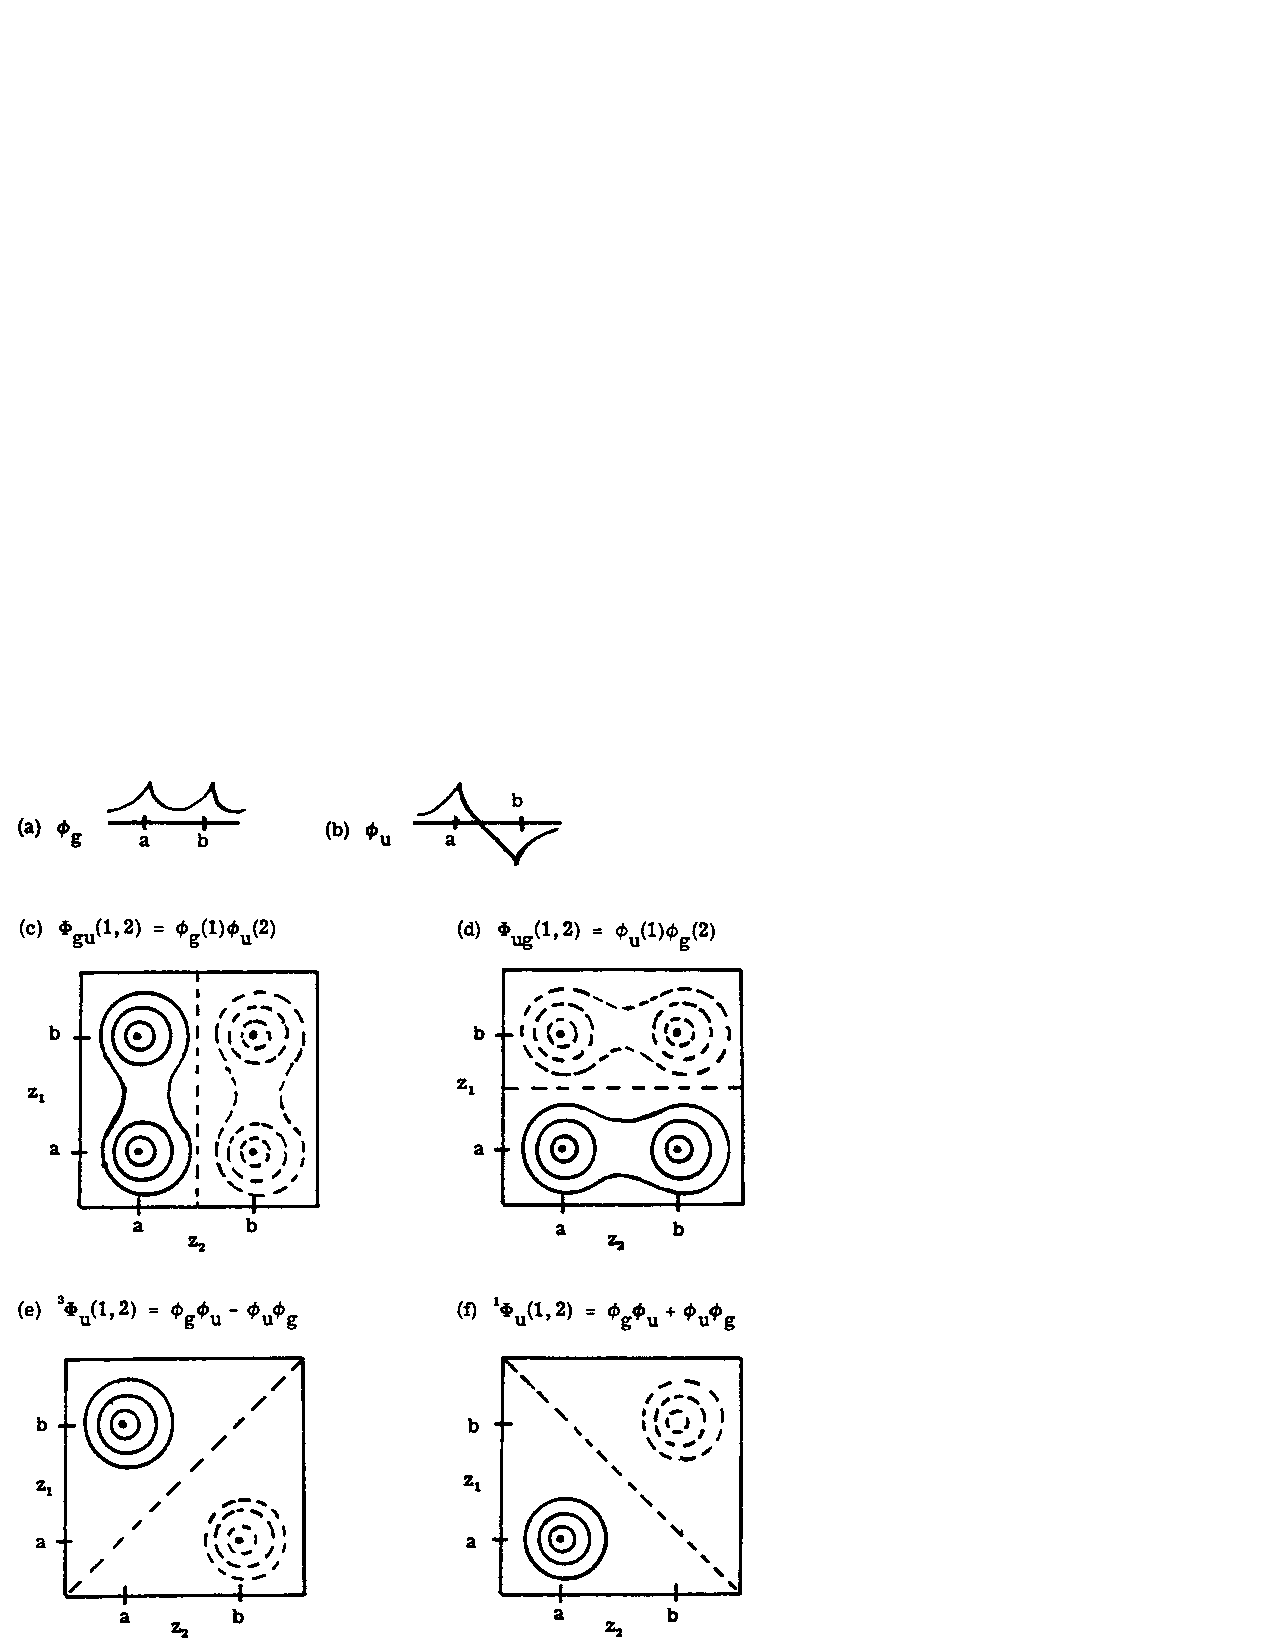
\includegraphics[scale=0.75]{fig2-21}
\caption{}
\label{fig2-21}
\end{figure}

In Figure \ref{fig2-21}, we compare the two-electron wavefunctions of
$\Phi_{gu}$, $\Phi_{ug}$, $^3\Phi_u$, and $^1\Phi_u$ All cases involve
a single nodal plane, and if there were no electron-electron
interactions, all of these wavefunctions would have the same total
energy. Note from equation (\ref{eqno2-26}) that both $u$ states have
the same total energy, and that any combination of these states leads
to the same one-electron energy, $h_{uu} + h_{gg}$. The difference
lies in the electron-electron interactions.  In Figure
\ref{fig2-21}(e), we see that the $^3\Phi_u$ wavefunction is zero
along the line with $z_1 = z_2$, whereas in Figure \ref{fig2-21}(f) we
see that the largest values (positive and negative) of $^1\Phi_u$
occur for $z_1 = z_2$. Since the electron repulsion term ${e^2 \over
r_{12}}$ is large and repulsive when the electrons are close, we see
that $^3\Phi_u$ is favored and $^1\Phi_u$ is disfavored. Indeed,
considering all possible combinations of $\Phi_{gu}$ and $\Phi_{ug}$,
the one with the lowest electron repulsion is just $^3\Phi_u$.  Thus,
the energy diagram for the molecular orbital wavefunctions of H$_2$,
becomes as in Figure \ref{fig2-22}.

\begin{figure}
\begin{center}
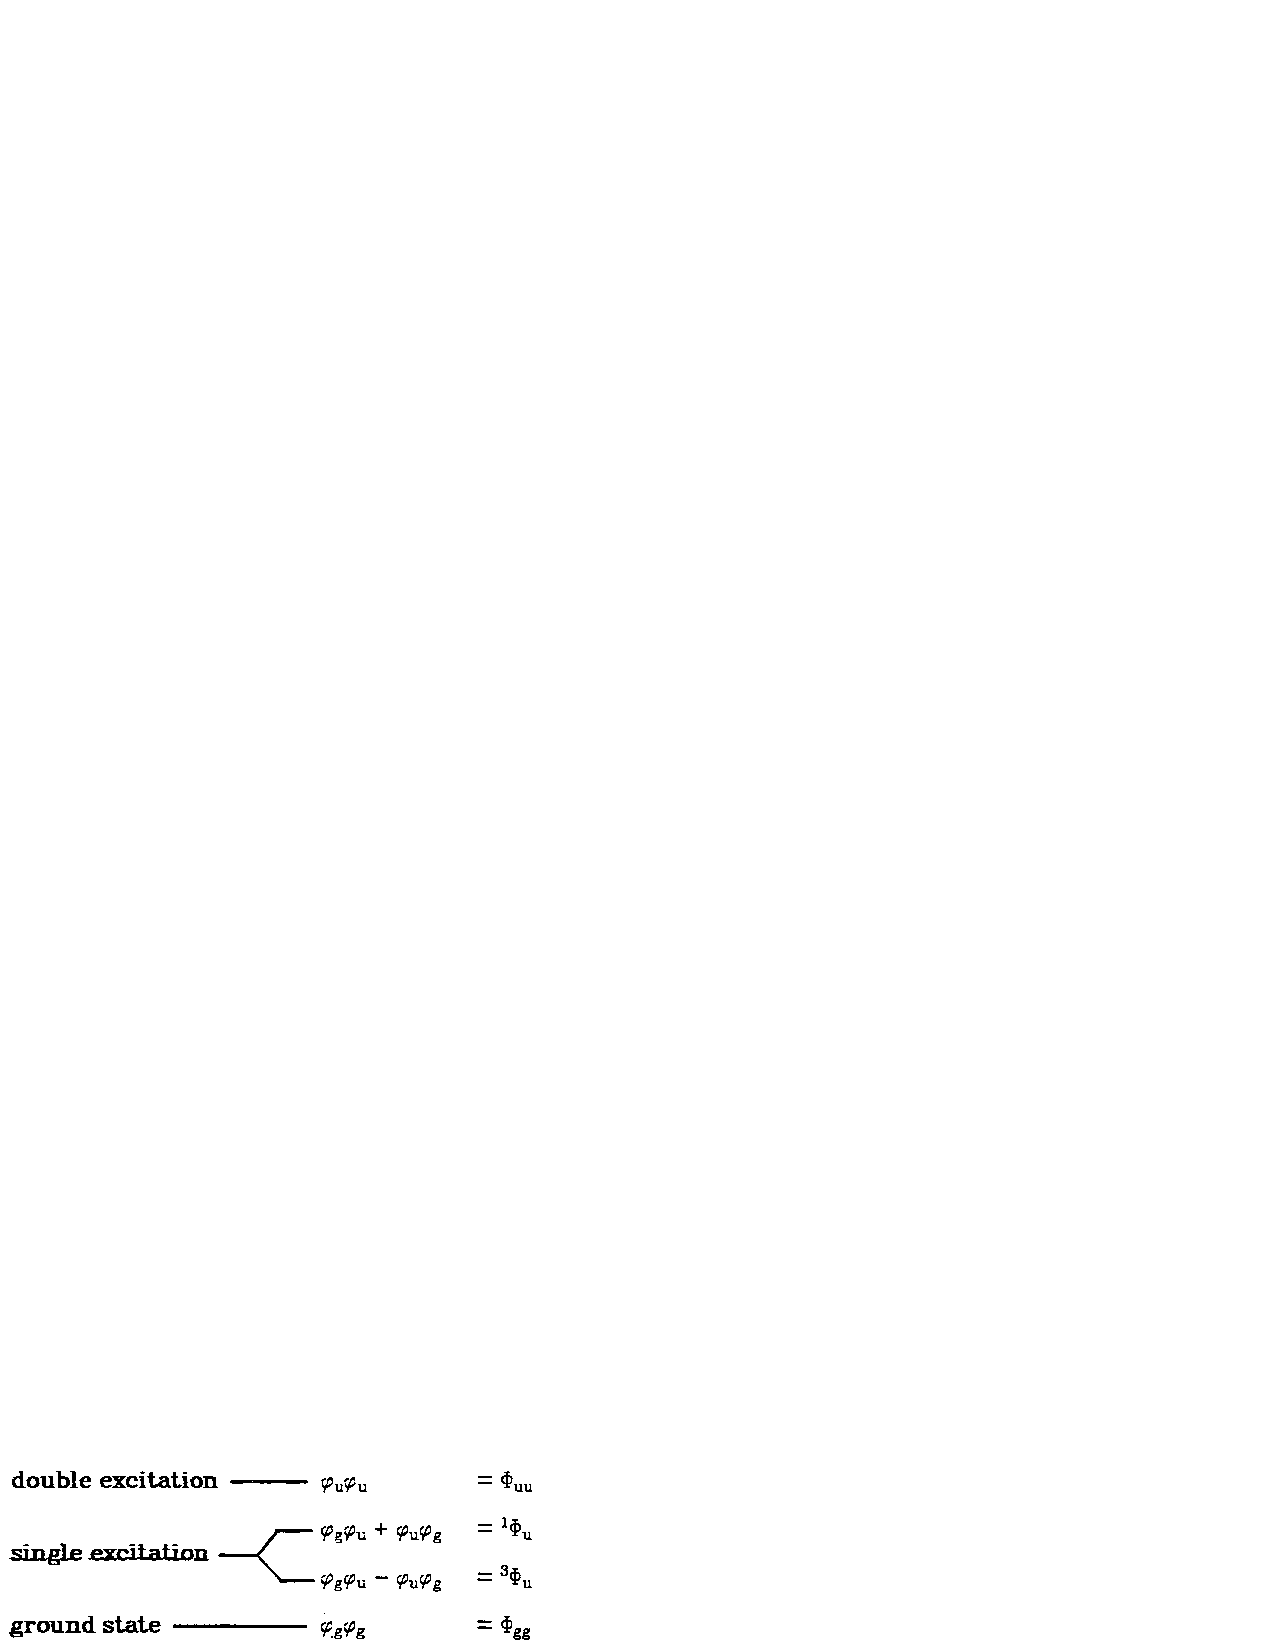
\includegraphics[scale=0.75]{fig2-22}
\end{center}
\caption{}
\label{fig2-22}
\end{figure}


\section{Quantitative Aspects}
    
Now that we see the physics behind why the $^3\Phi_u$ wavefunction
(\ref{eqno2-30}) is the best $u$ state, we will examine the
quantitative energy expression
\begin{eqnarray}
E( ^3\Phi_u) &=& {\langle ^3\Phi_u \vert {\hat H}\vert ^3\Phi_u
\rangle \over \langle ^3\Phi_u \vert ^3\Phi_u \rangle} = {\langle gu -
ug \vert {\hat H} \vert gu - ug \rangle \over \langle gu - ug \vert gu
- ug \rangle}\cr &=& {2 \langle gu \vert {\hat H} \vert gu - ug
\rangle \over 2 \langle gu \vert gu - ug \rangle} = {\langle gu \vert
{\hat H} \vert gu \rangle - \langle gu \vert {\hat H} \vert ug \rangle
\over \langle gu \vert gu \rangle - \langle gu \vert ug \rangle}.
\end{eqnarray}
Since
\begin{equation}
\langle gu \vert ug \rangle = \langle g \vert u \rangle \langle u 
\vert g \rangle = 0
\end{equation}
\begin{equation}
\langle gu \vert h ( 1 ) \vert ug \rangle = \langle g \vert h \vert 
u \rangle \langle u \vert g \rangle = 0
\end{equation}
\begin{equation}
\langle gu \vert h ( 2 ) \vert ug \rangle = \langle g \vert u 
\rangle \langle u \vert h \vert g \rangle = 0,
\end{equation}
we are left with
\begin{equation}
E \left( ^3\Phi_u \right) = E_{gu} - \langle gu \vert {\hat H} \vert 
ug \rangle,
\label{e_trip_u}
\end{equation}
where
\begin{equation}
\langle gu \vert {\hat H} \vert ug \rangle = \langle gu \vert {1 \over 
r_{12}} \vert ug \rangle = \int \int d^3 r_1 d^3 r_2 {\varphi^*_g ( 1 ) 
\varphi_u ( 1 ) \varphi^*_u ( 2 ) \varphi_g ( 2 ) \over r_{12}} 
= K_{gu},
\label{eqno2-32}
\end{equation}
where this two-electron term is called the \emph{exchange integral}
between orbitals $\varphi_g$ and $\varphi_u$. The net result is
\begin{equation}
E \left( {^3\Phi}_u \right) = E_{gu} - K_{gu}
\end{equation}
and
\begin{equation}
E \left( {^1\Phi}_u \right) = E_{gu} + K_{gu}.
\end{equation}
Since the previous section showed that
\begin{equation}
E \left( {^1\Phi}_u \right) > E \left( {^3\Phi}_u \right),
\end{equation}
we see that the exchange integral must be positive, $K_{gu} \geq 0$.

What is the physical significant of $K_{gu}$? It tells us how much the
two-electron energy changes when we go from the wavefunctions in
Figure \ref{fig2-21}(c), or \ref{fig2-21}(d), to the wavefunctions in
Figure \ref{fig2-21}(e), or \ref{fig2-21}(f). Thus, the $K_{gu}$ is
the quantitative representation of our earlier argument that
$^3\Phi_u$ has a better two-electron energy than $^1\Phi_u$. It is
better by precisely $2K_{gu}$.

Another way to look at this is to substitute equation (\ref{eqno2-26})
into (\ref{e_trip_u}), leading to
\begin{equation}
E \left(^3\Phi_u\right) = \left[ h_{gg} + h_{uu} + {1 \over R} 
\right] + \left[ J_{gu} - K_{gu}\right]
\end{equation}
\begin{equation}
E \left(^1\Phi_u\right) = \left[ h_{gg} + h_{uu} + {1 \over R} 
\right] + \left[ J_{gu} + K_{gu}\right]
\end{equation}
Here $J_{gu} - K_{gu}$ is the total two-electron energy of Figure
\ref{fig2-21}(f), while $J_{gu} + K_{gu}$ is the total two-electron
energy of Figure \ref{fig2-21}(e), and $J_{gu}$ is the two-electron
energy of Figures \ref{fig2-21}(c) and \ref{fig2-21}(d). The
two-electron energy of $^3\Phi_u$ can also be written as
\begin{equation}
J_{gu} - K_{gu} = {\langle {^3\Phi}_u \vert {1 \over r_{12}} \vert
{^3\Phi}_u \rangle \over  \langle {^3\Phi}_u \vert {^3\Phi}_u 
\rangle} = \int \int d^3 r_1 d^3 r_2 {^3P_u(1,2) \over 
r_{12}},
\label{eqno2-33}
\end{equation}
where $1/2$ comes from $\langle {^3\Phi}_u \vert^3\Phi_u \rangle = 2$,
and where
\begin{equation}
{^3P}_u ( 1 , 2 ) = {1 \over 2} {^3\Phi}_u^* ( 1 , 2 ) ^3\Phi_u(1,2).
\end{equation}
Since ${^3P}_u$ is the absolute square of ${^3\Phi}_u$, it is
positive for all possible values of $r_1$ and $r_2$.  Since the
integral in equation (\ref{eqno2-33}) is always positive, we see that
the total two-electron energy of the ${^3\Phi}_u$ state must be
positive
\begin{equation}
J_{gu} - K_{gu} \geq 0,
\end{equation}
and hence
\begin{equation}
J_{gu} \geq K_{gu}
\label{eqno2-34}
\end{equation}
the exchange integral is always less than the Coulomb
integral. Combining (\ref{eqno2-34}) with $J_{ij} \geq 0$, leads then
to
\begin{equation}
J_{gu} \geq K_{gu} \geq 0.
\end{equation}
This relation is true for any pairs of orbitals, as shown in Section
\ref{appendix-b}. 

\subsection{Potential Curves}
    
So far we have discussed the MO wavefunction assuming
that the bonding orbital $\varphi_g$ is much better than the
antibonding orbital $\varphi_u$. This is true for shorter internuclear
distance $R$ but does not remain true as the bond is broken. Thus, in
Figure \ref{fig2-23} we compare the energy of the molecular orbital
wavefunction $\Phi_{gg}$ with the exact energy for the ground state of
H$_2$. This molecular orbital wavefunction leads to a good value for
the bond length but a very bad description of the processes of
breaking the bond.

\begin{figure}
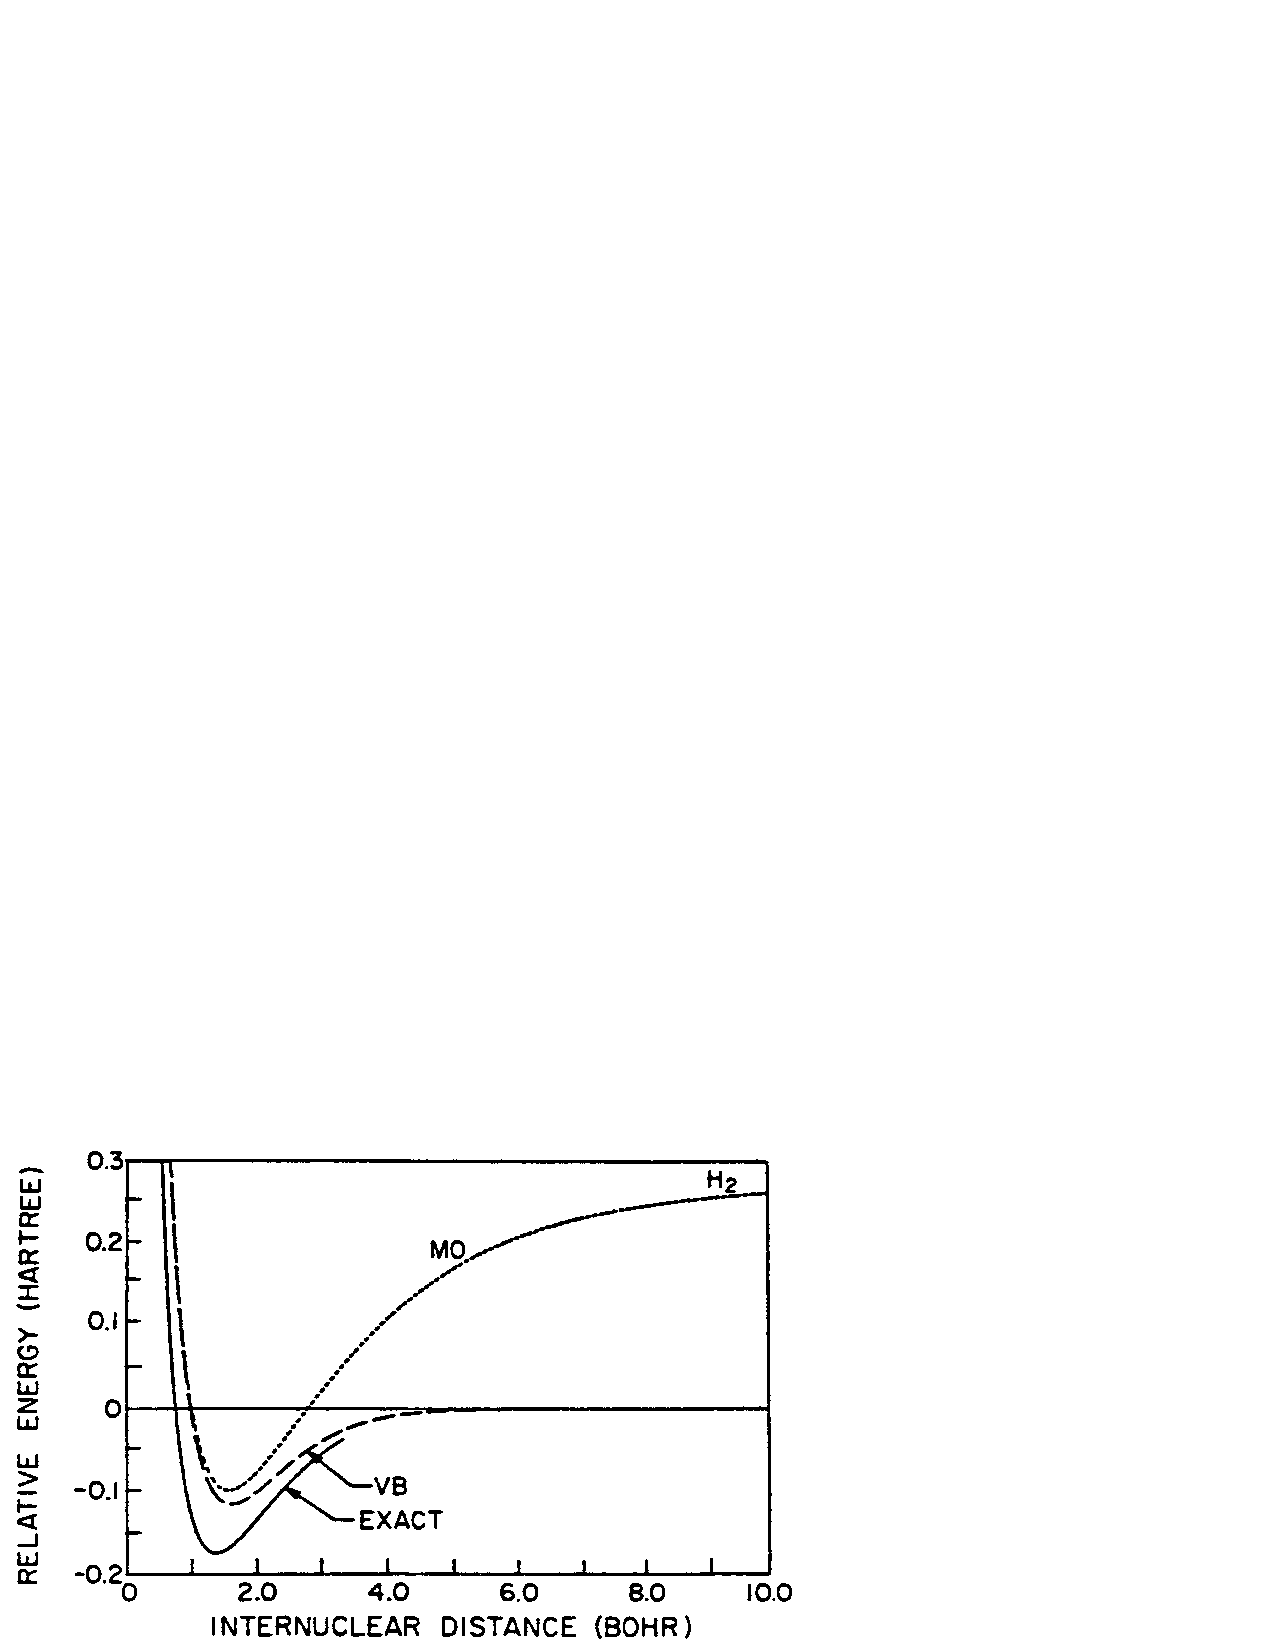
\includegraphics[scale=0.75]{fig2-27}
\caption{The energy of the MO wave function for the ground state of
  H$_2$ with comparison to the VB and exact energies.}
\label{fig2-23}
\end{figure}
    
The origin of this problem can be seen by substituting the AO
description of the MO (\ref{eqno2-19a})--(\ref{eqno2-19b}) into the MO
wavefunction (\ref{eqno2-18}), leading to
\begin{equation}
\Phi^{MO}_{gg} ( 1 , 2 ) = N \left[ \chi_\ell \chi_\ell + \chi_r \chi_r + 
\chi_\ell \chi_r + \chi_r \chi_\ell \right] = \Phi_{covalent} + 
\Phi_{ionic},
\label{eqno2-35}
\end{equation}
where $N = [2(1+S)]^{-1}$ and
\begin{equation}
\Phi_{covalent} = N \left( \chi_\ell \chi_r + \chi_r \chi_\ell 
\right)
\label{eqno2-36}
\end{equation}
\begin{equation}
\Phi_{ionic} = N \left( \chi_\ell \chi_\ell + \chi_r \chi_r \right).
\end{equation}
At very large $R$, the exact wavefunction will have one electron near
the left proton and one at the right, as in equation (\ref{eqno2-36}),
which we will refer to as the \emph{covalent} part of the
wavefunction. The other terms of (\ref{eqno2-35}) have both electrons
near one proton and none near the other, thus an \emph{ionic}
wavefunction. At $R = \infty$, these ionic terms lead to the energy of
H$^-$ and H$^+$ rather than the energy of two hydrogen atoms. Since
the MO wavefunction must have equal covalent and ionic
contributions, it yields terrible energies for large $R$.
    
The basic problem with the molecular orbital wavefunction is that both
electrons are in the same $\varphi_g$ orbital, and hence, each
electron has an equal probability of being on either center,
regardless of the instantaneous location of the other electron. In the
exact wavefunction, the motions of the electrons tend to be correlated
so that if one electron is on the left, the other tends to be on the
right. This correlation is necessarily ignored in the molecular
orbital wavefunction, and the resulting error is often referred to as
the \emph{correlation error}.  For small $R$, the two centers are
close to each other, and this neglect of correlation is not so
important. At $R = \infty$, however, the correlation of electrons is
of paramount importance and neglect of correlation leads to
ludicrously poor wavefunctions.
    
In the next section, we will discuss a simple wavefunction, the valence bond
wavefunction, that eliminates this problem of describing large $R$.

\section{The Valence Bond Description of H$_2$}

\subsection{The Covalent States}
    
We will now re-examine the ground state of H$_2$ molecule. However,
rather than the approach of the previous section, plotting electrons
one by one into the orbital of H$^+_2$, we will instead start with the
exact wavefunction at $R = \infty$. This, of course, consists of two
hydrogen atoms infinitely far apart, say electron 1 on the left, and
electron 2 on the right, as in Figure \ref{fig2-24}. The wavefunction
for Figure \ref{fig2-24} is
\begin{equation}
\Phi_g \left( {\bf r}_1 , {\bf r}_2 \right) = \chi_\ell ( {\bf r}_1 ) 
\chi_r ( {\bf r}_2),
\label{eqno2-37}
\end{equation}
where
\begin{equation}
\chi_\ell ( {\bf r}_1 ) = Ne^{-{\bf r}_{a1}}
\label{eqno2-38a}
\end{equation}
\begin{equation}
\chi_r( {\bf r}_2) = Ne^{- {\bf r}_{b2}}
\label{eqno2-38b}
\end{equation}
and $N$ is the normalization factor.

\begin{figure}
\begin{center}
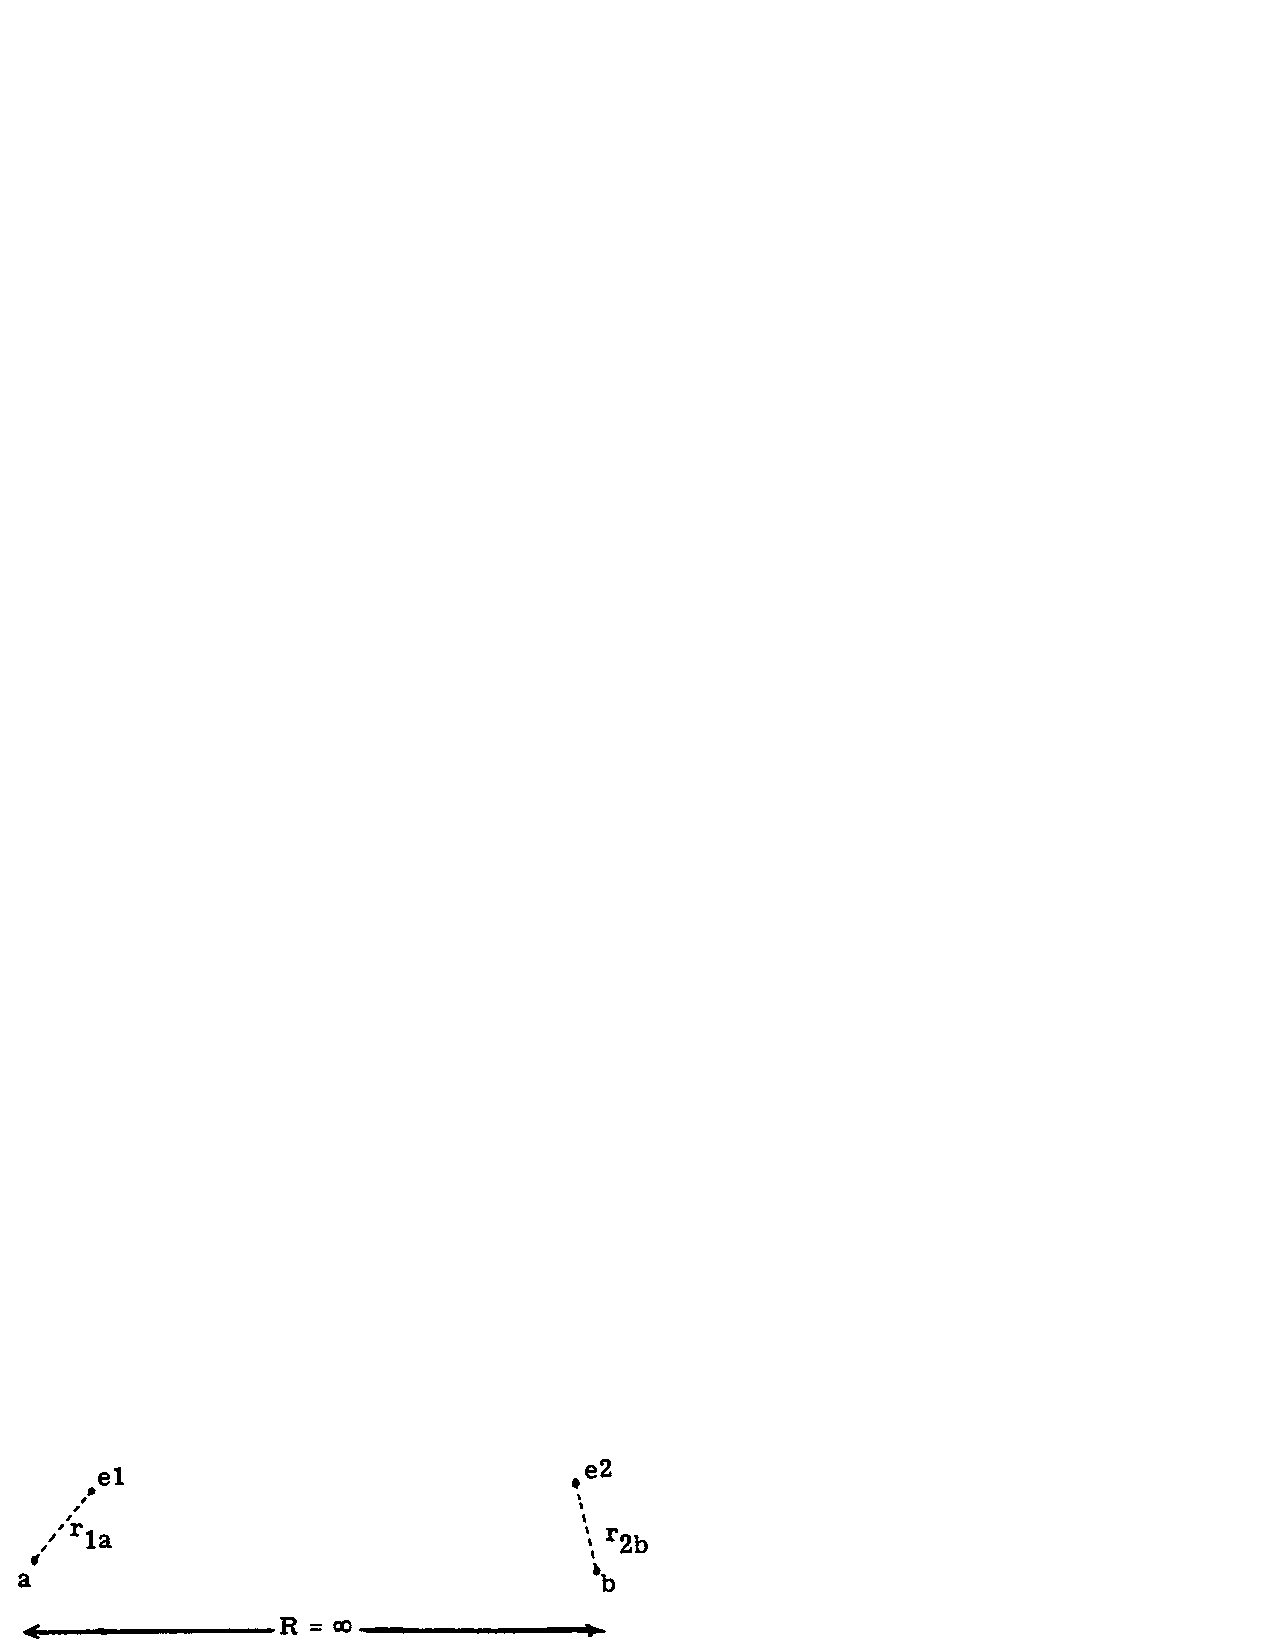
\includegraphics[scale=0.75]{fig2-24}
\end{center}
\caption{}
\label{fig2-24}
\end{figure}
    
This wavefunction $\Phi_a$ says that the probability of electron 1 being 
at a particular position, is independent of where electron 2 is, and vice 
versa. Since the atoms are infinitely far apart, the electrons should not be 
influence by each other.
    
There is a second wavefunction that is just as good, or as bad, as in 
(37), namely,
\begin{equation}
\Phi_b ( {\bf r}_1 , {\bf r}_2 ) = \chi_r ({\bf r}_1) \chi_\ell ( {\bf 
r}_2),
\end{equation}
where the electrons have been interchanged. This wavefunction $\Phi_b$ 
is different from $\Phi_a$ since electron 1 is on the opposite sides of 
the universe. However, the energies of $\Phi_b$ and $\Phi_a$ 
must be the same, since electrons 1 and 2 have the same properties.
    
We will find it useful to combine $\Phi_a$ and $\Phi_b$ into two new 
wavefunctions,
\begin{equation}
\Phi_g ( 1 , 2 ) = \Phi_a ( 1 , 2 ) + \Phi_b ( 1 , 2 ) = \chi_\ell ( 
1 ) \chi_r ( 2 ) + \chi_r ( 1 ) \chi_\ell ( 2 )
\label{eqno2-39a}
\end{equation}
\begin{equation}
\Phi_u ( 1 , 2 ) = \Phi_a ( 1 , 2 ) - \Phi_b ( 1 , 2 ) = \chi_\ell ( 
1 ) \chi_r ( 2 ) - \chi_r ( 1 ) \chi_\ell ( 2 )
\label{eqno2-39b}
\end{equation}
unnormalized, because at finite $R$ these are the optimum wavefunctions. 
Before examining the energies, we need to understand how to think about 
the relative locations of the electrons in these wavefunctions.
    
\begin{figure}
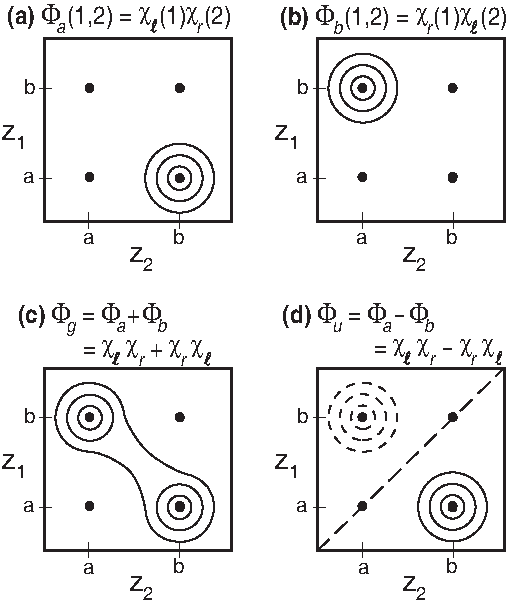
\includegraphics[scale=0.75]{fig2-25}
\caption{(a) $\Phi_a(1,2)=\chi_\ell(1)\chi_r(2)$; 
(b) $\Phi_b(1,2)=\chi_r(1) \chi_\ell(2)$;
(c) $\Phi_g=\Phi_a+\Phi_b=\chi_\ell\chi_r+\chi_r\chi_\ell$;
(d) $\Phi_u=\Phi_a+\Phi_b=\chi_\ell\chi_r-\chi_r\chi_\ell$}
\label{fig2-25}
\end{figure}
    
In Figure \ref{fig2-25}, we plot the four wavefunctions, $\Phi_a$,
$\Phi_b$, $\Phi_g$, and $\Phi_u$.  Here we see that $\Phi_u$ has a
nodal plane, corresponding to $z_1 = z_2$, while $\Phi_g$ does
not. Indeed, along the line between the two peaks in Figure
\ref{fig2-25}(c), we see that the gradient of the $\Phi_g$
wavefunction is smaller than that of $\Phi_a$ or $\Phi_b$, while the
gradient of the wavefunction is larger. This decrease in the gradient
of $\Phi_g$, and increase for $\Phi_u$, depends upon $R$ with a bigger
effect for smaller $R$. Thus, based on kinetic energy, we would expect
that $\Phi_g$ is bonding and $\Phi_u$ is antibonding, and indeed this
is the case, as shown in Figure \ref{fig2-26}.

\begin{figure}
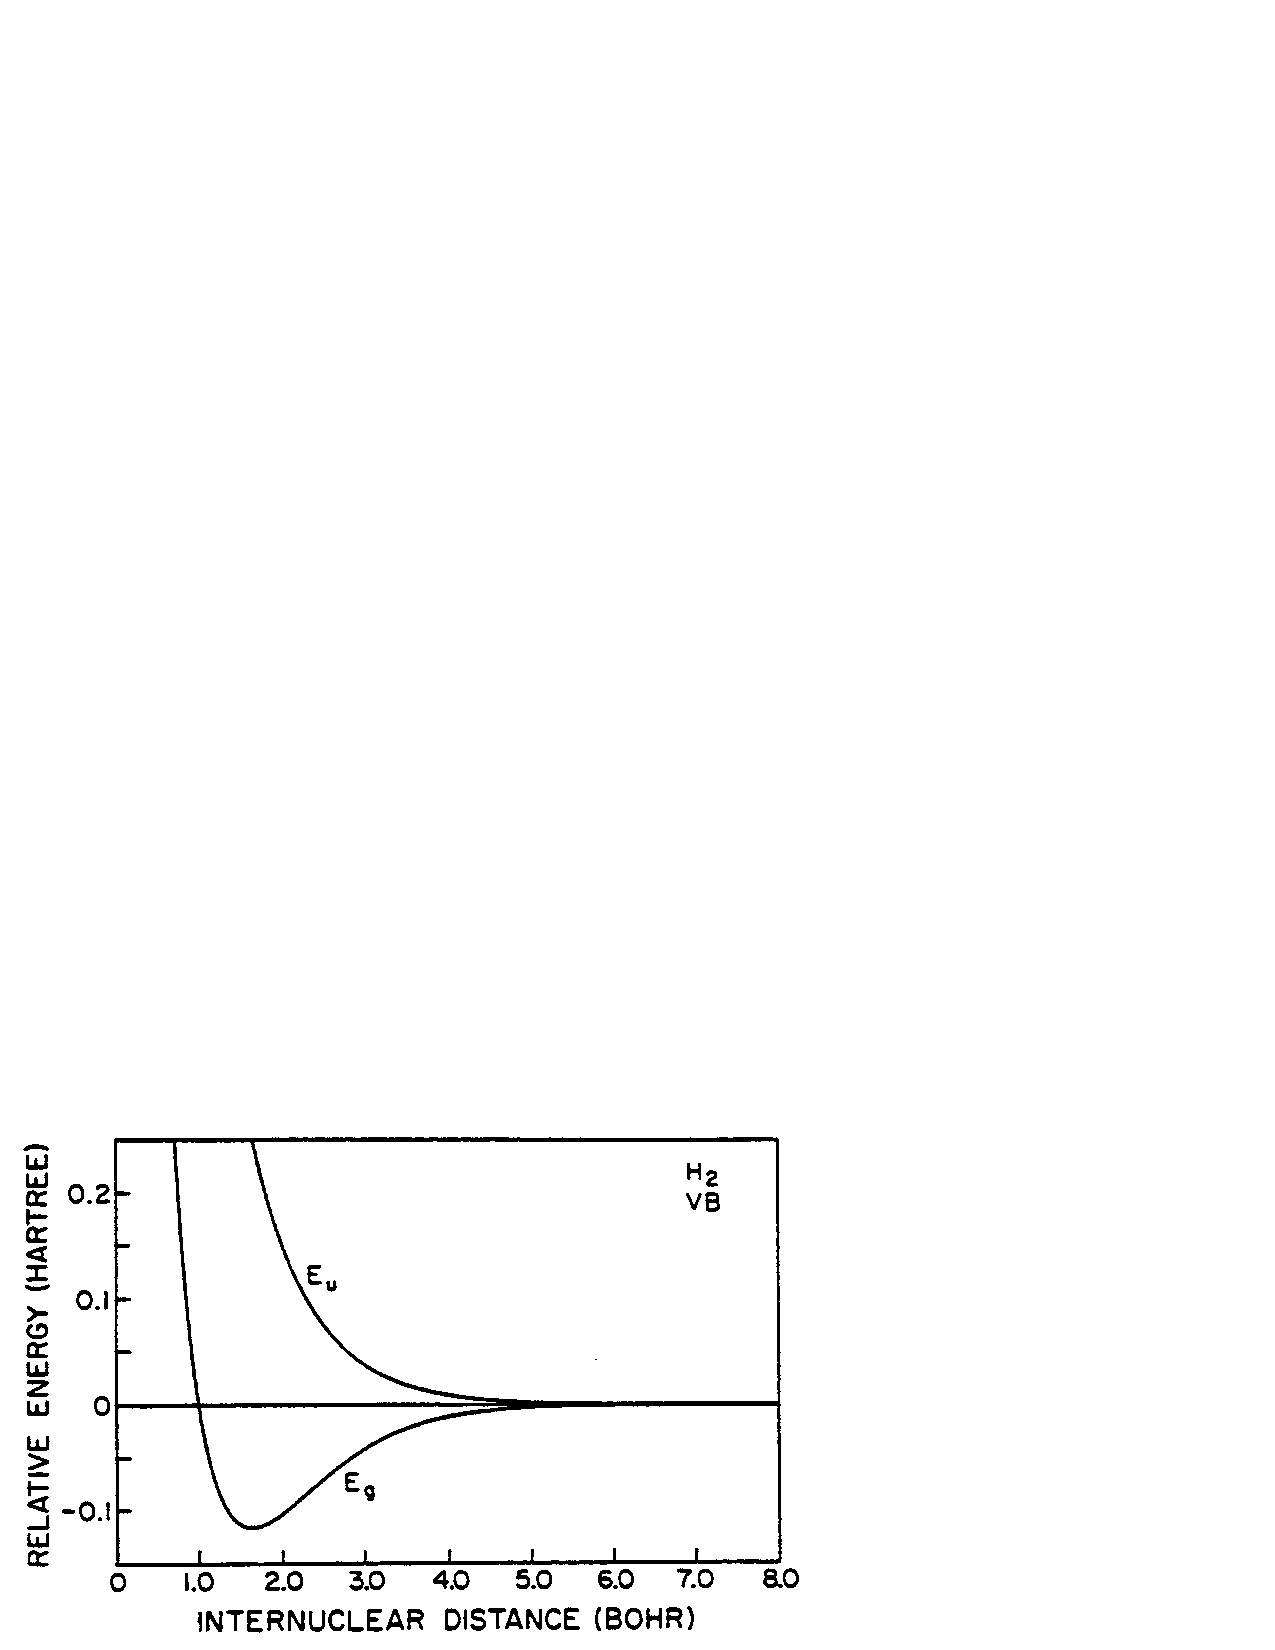
\includegraphics[scale=0.75]{fig2-26}
\caption{The energies $E_g$ and $E_u$ for the valence bond wave
  functions of H$_2$.}
\label{fig2-26}
\end{figure}

\subsection{Symmetry}
    
Inversion of the coordinates of the electrons $r_{a1} \leftrightarrow
r_{b1}$ and $r_{a2} \leftrightarrow r_{b2}$ leads to (see equations
(\ref{eqno2-38a})--(\ref{eqno2-38b}))
\begin{equation}
\chi_\ell \left( {\bf r}_1 \right) \leftrightarrow \chi_r \left( {\bf 
r}_1 \right).
\end{equation}
Consequently,
\begin{equation}
{\hat{I}} \Phi_a \left( {\bf r}_1, {\bf r}_2 \right) = \chi_r 
\left( {\bf r}_1 \right) \chi_\ell \left( {\bf r}_2 \right) = \Phi_b 
\left( {\bf r}_1 , {\bf r}_2 \right)
\end{equation}
or ${\hat{I}} \Phi_b = \Phi_a$.  As a result,
\begin{equation}
{\hat{I}} \Phi_g = I \left( \Phi_a + \Phi_b \right) = \left( \Phi_b + 
\Phi_a \right) = \Phi_g
\end{equation}
\begin{equation}
{\hat{I}} \Phi_u = I \left( \Phi_a - \Phi_b \right) = \left( \Phi_b - 
\Phi_a \right) = - \Phi_u ,
\end{equation}
and we see that $\Phi_g$ and $\Phi_u$ are indeed gerade and ungerade, 
respectively.

\subsection{Comparison of VB and MO Wavefunctions}

\subsubsection{Ground State}

The MO wavefunction is (ignoring normalization)
\begin{equation}
\Phi^{MO}_{gg} ( 1 , 2 ) = \varphi_g ( 1 ) \varphi_g ( 2 ) = \left[ 
\chi_\ell \chi_r + \chi_r \chi_\ell \right] + \left[ \chi_\ell \chi_\ell + \chi_r 
\chi_r \right] ,
\end{equation}
whereas the VB wavefunction is
\begin{equation}
\Phi^{VB} ( 1 , 2 ) = \left[ \chi_\ell \chi_r + \chi_r \chi_\ell \right] .
\end{equation}
The energies for these wavefunctions are compared in Figure
\ref{fig2-27}, where we see that the valence bond is always better,
but that the difference becomes negligible for small $R$.

\begin{figure}
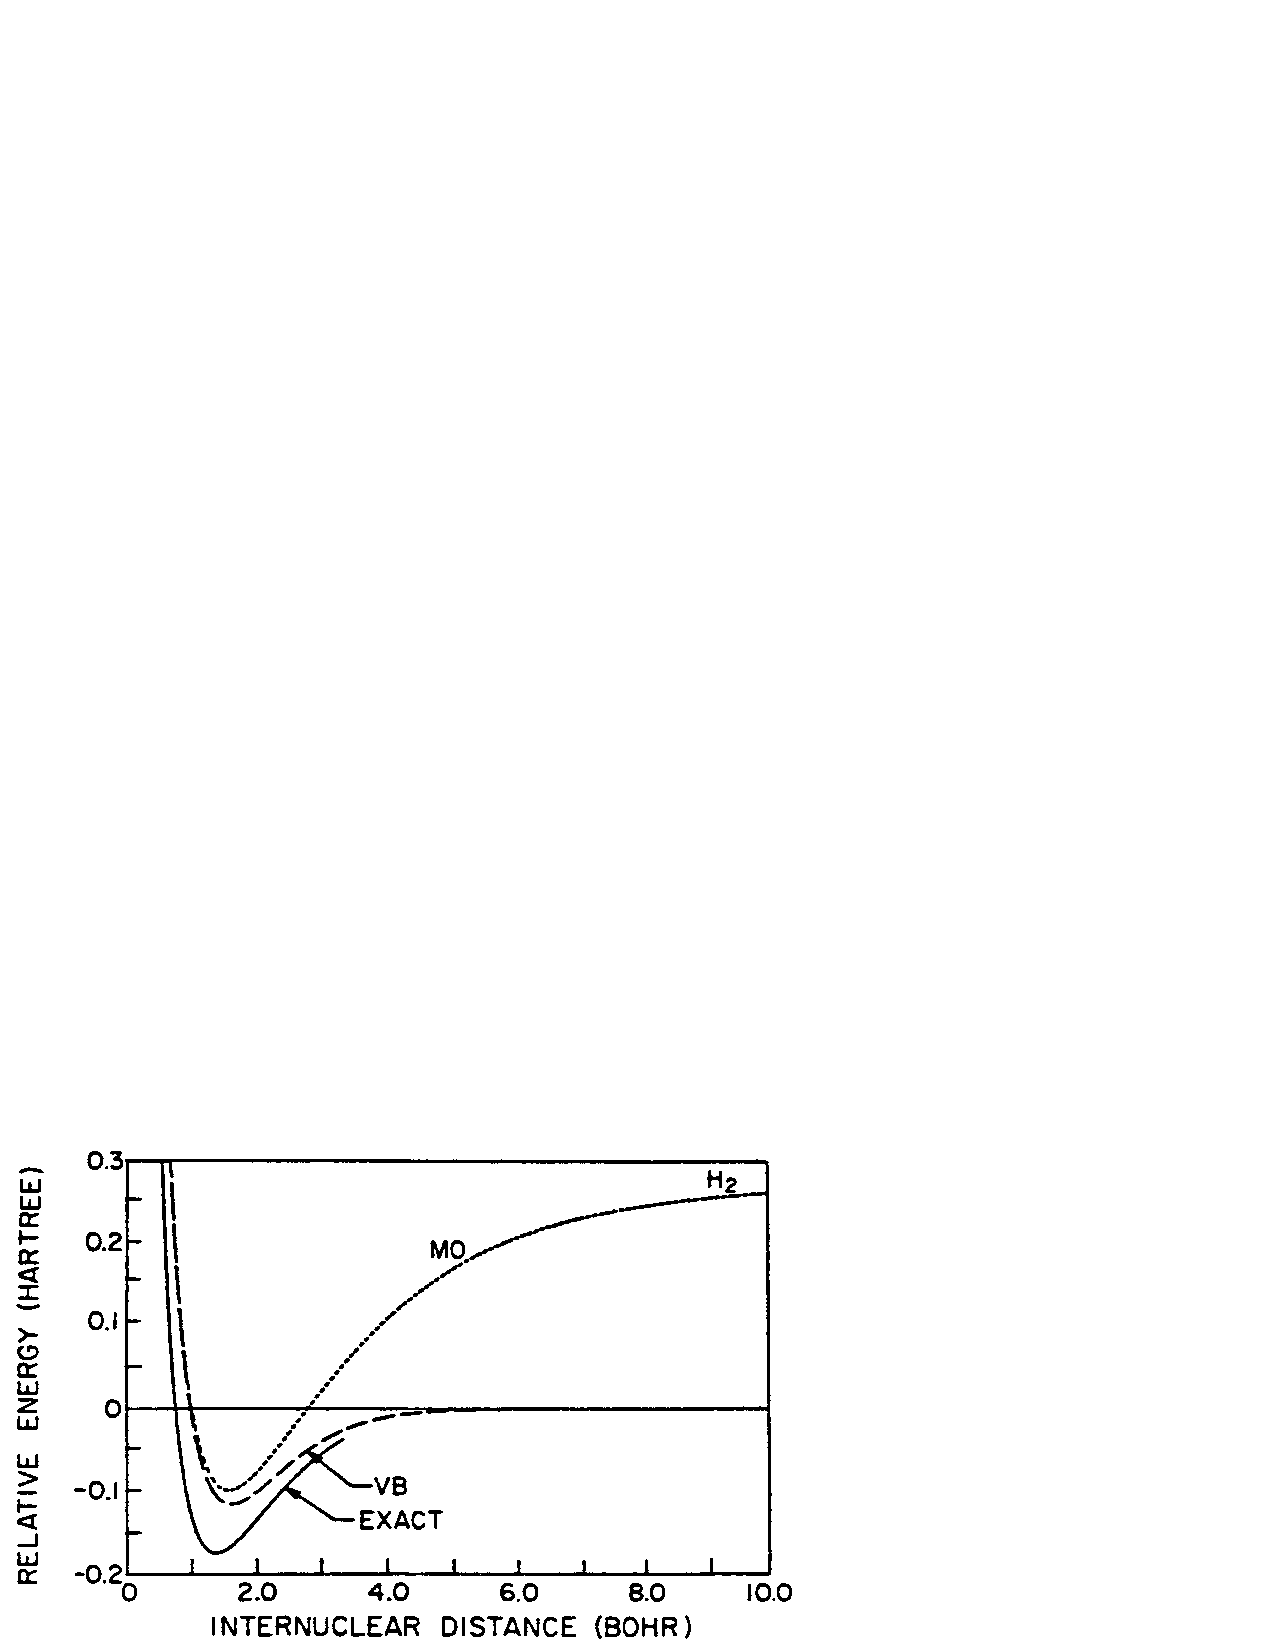
\includegraphics[scale=0.75]{fig2-27}
\caption{The energy of the MO wave function for the ground state of
  H$_2$ with comparison to the VB and exact energies.}
\label{fig2-27}
\end{figure}

\begin{figure}
\begin{center}
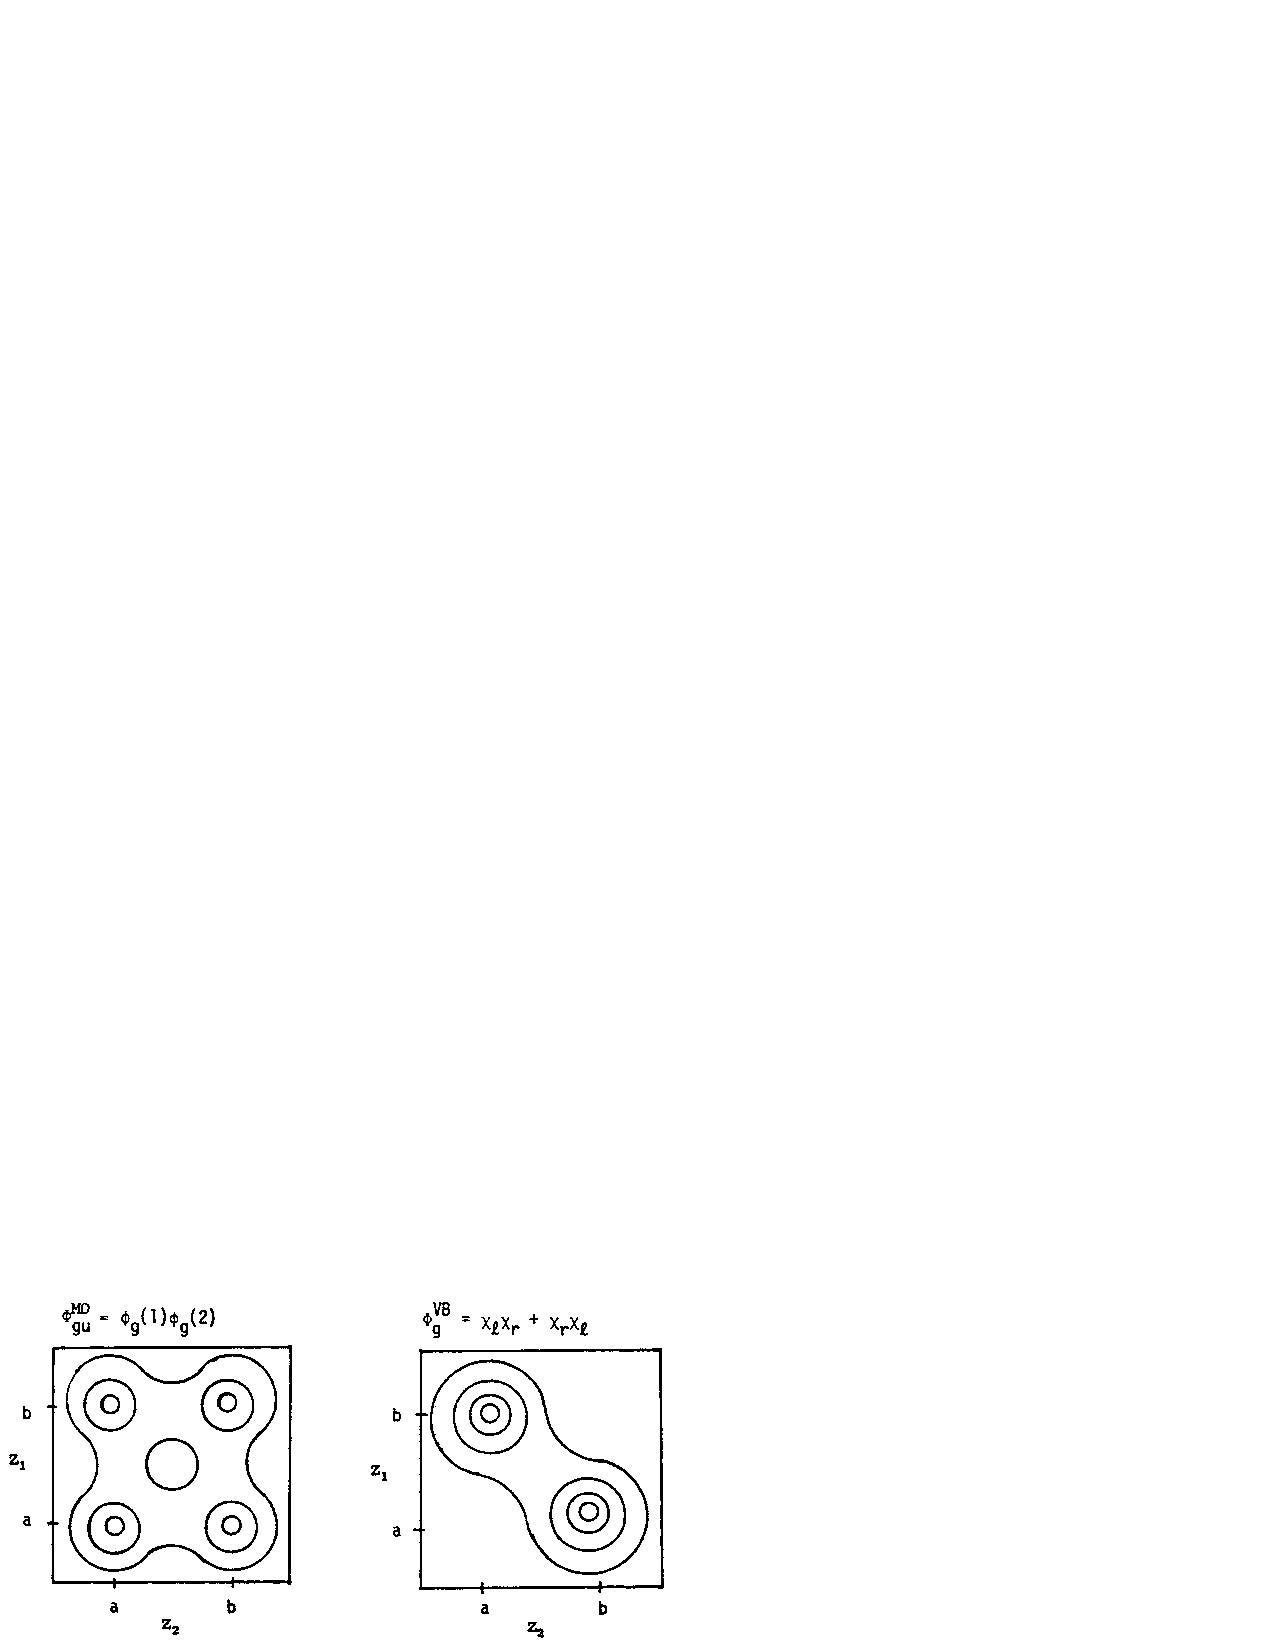
\includegraphics[scale=0.75]{fig2-28}
\end{center}
\caption{ (a) $\Phi^{MO}_{gu} = \varphi_g ( 1 ) \varphi_g(2)$
(b) $\Phi^{VB}_g = \chi_\ell \chi_r + \chi_r \chi_\ell$.}
\label{fig2-28}
\end{figure}

The wavefunctions are compared in Figure \ref{fig2-28}, showing
graphically, how the valence bond wavefunction has smaller probability
of having $z_1 = z_2$, leading to the lower electron repulsion
energies. On the other hand, the molecular orbital wavefunction is
smoother, leading to smaller kinetic energies.  For normal bond
distances, the electron repulsion effects dominate so that the valence
bond wavefunction is better. However, for very short $R$, the kinetic
energy becomes dominant so that the molecular orbital and valence bond
wavefunctions lead to nearly identical total energies.

\subsubsection{The $u$ States}

Expanding the MOs in terms of AOs, ignoring
normalization, leads to
\begin{equation}
\Phi_{gu} = \left( l + r \right) \left( l - r \right) = ll + rl - lr - 
rr
\end{equation}    
\begin{equation}
\Phi_{ug} = \left( l - r \right) \left( l + r \right) = ll - rl + lr - 
rr .
\end{equation}   
Thus
\begin{equation}
{^3}\Phi_u = \Phi_{gu} - \Phi_{ug} = 2 \left( r l - l r \right) = 
\Phi^{VB}_u
\end{equation}
\begin{equation}
{^1}\Phi_u = gu + ug = 2 \left( l l - r r \right) = 
\Phi^{ION}_u .
\end{equation}  
That is, the first excited state of the MO description
$^3\Phi_u$, is identical to the first excited state in the valence
bond description. Both describe a covalent repulsive state that
separates to two free $H$ atoms, as indicated in Figure
\ref{fig2-29}. 

\begin{figure}
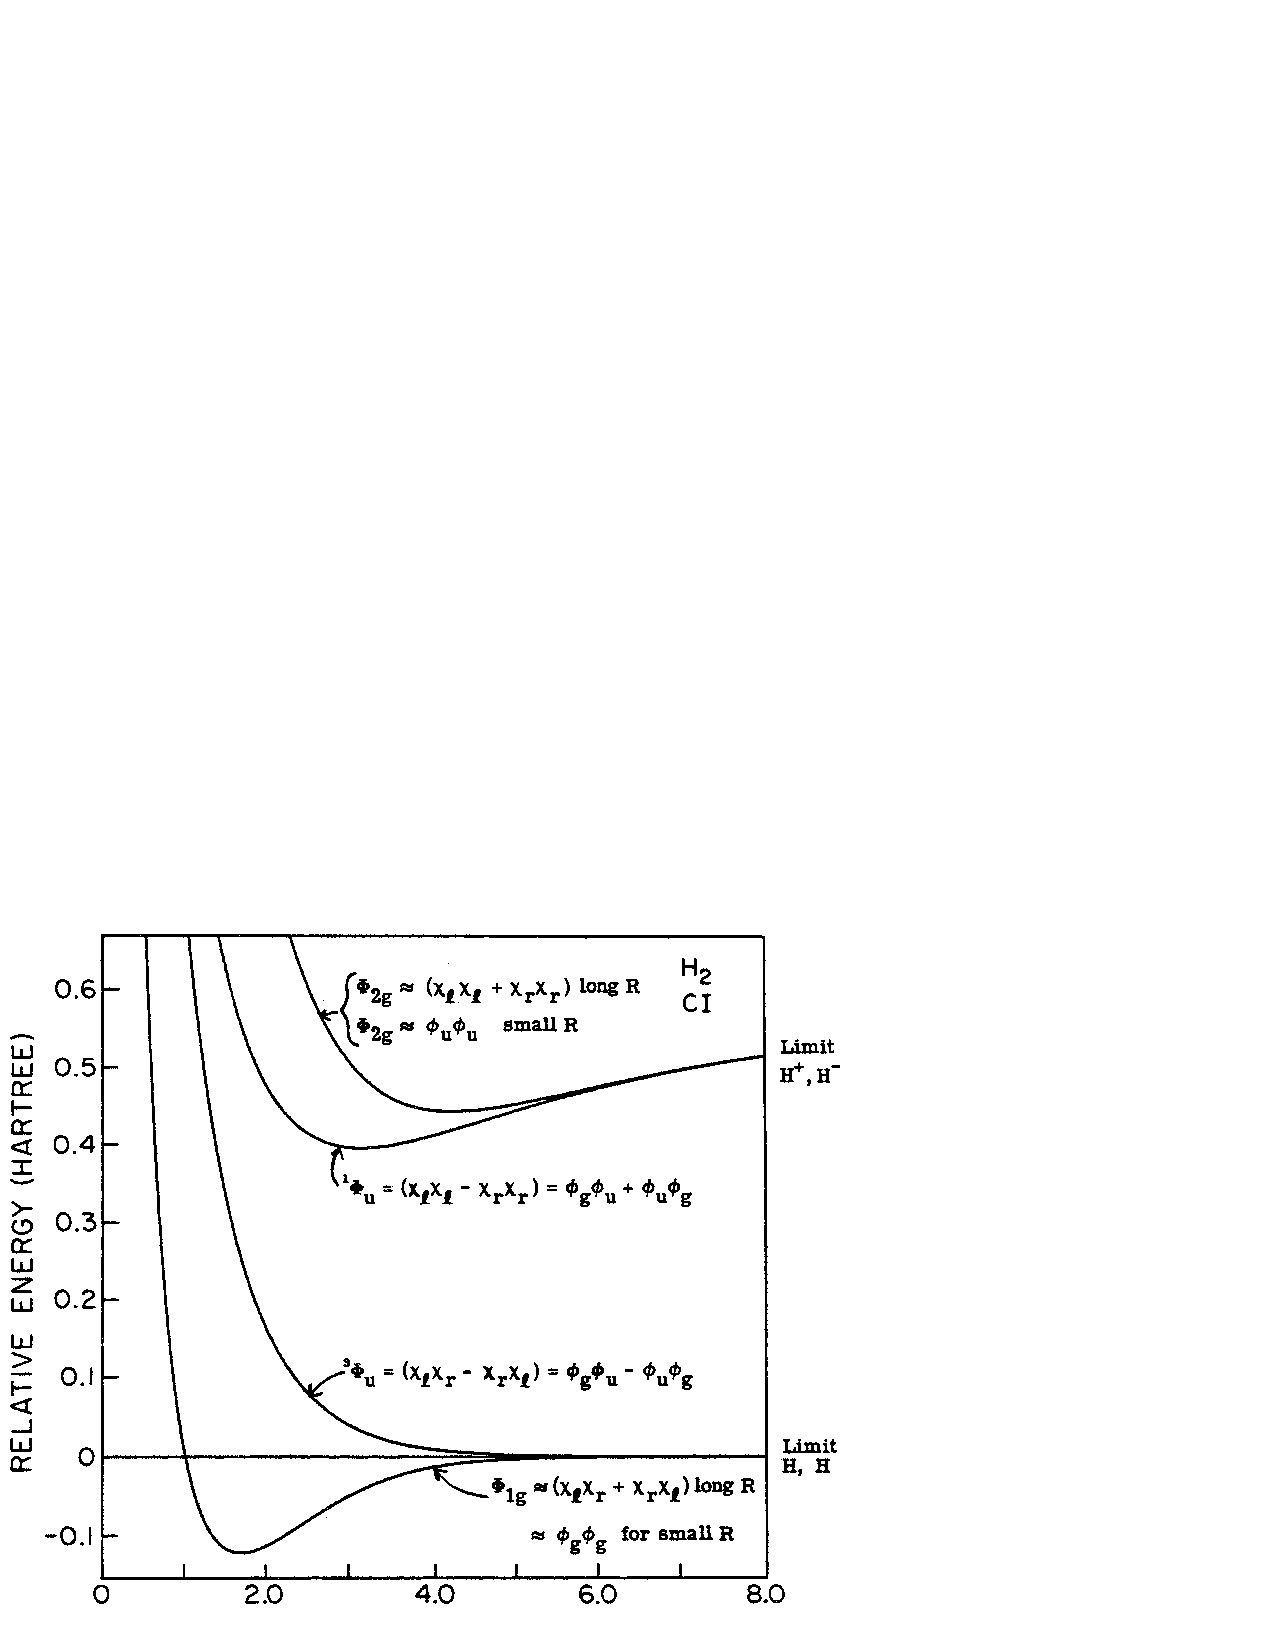
\includegraphics[scale=0.75]{fig2-29}
\caption{Energies for the states of H$_2$, using atomic orbitals
  ($\zeta = 1.0$).}
\label{fig2-29}
\end{figure}

\subsubsection{The Second $g$ State}

In the MO description
\begin{equation}
\Phi^{MO}_{uu} = \left( l - r \right) \left( l - r \right) = {\left[ 
\left( ll + rr \right) - \left( lr + rl \right) \right] \over 2 
\left( 1 - S \right)}
\label{eqno2-40a}
\end{equation}
\begin{equation}
\Phi^{MO}_{gg} = \left( l + r \right) \left( l + r \right) = {\left[ 
\left( ll + rr \right) + \left( lr + rl \right) \right] \over 2 
\left( 1 + S \right)}
\label{eqno2-40b}
\end{equation}
(now we include normalization factors). In contrast, the VB
description leads to
\begin{equation}
\Phi^{VB}_g = { \left( l r + r l \right) \over \sqrt{2 \left( 1 + 
S^2 \right)}}
\label{eqno2-41}
\end{equation}
\begin{equation}
\Phi^{ION}_g = { \left( l r + r r \right) \over \sqrt{2 \left( 1 + 
S^2 \right)}}
\end{equation}
for the covalent and ionic $g$ states.
    
The connections between these states are
\begin{eqnarray}
\Phi^{VB}_g &=& {1 \over \sqrt{2(1+S^2)}} \left[ \left( 1 + S \right) 
\Phi^{MO}_{gg} - \left( 1 - S \right) \Phi^{MO}_{gg} \right]\cr
&=& {(1+S) \over \sqrt{2(1+S^2)}} \left[ \Phi^{MO}_{gg} - \lambda 
\Phi^{MO}_{uu} \right],
\end{eqnarray}
where
\begin{equation}
\lambda = {1 - S \over 1 + S} .
\end{equation}

Thus, we can fix up the MO wavefunction so that it behaves like the VB
wavefunction, by mixing together the $\Phi^{MO}_{gg}$ and
$\Phi^{MO}_{uu}$ wavefunctions. This is related to the configuration
interaction (CI) wavefunction, as discussed below.  For large $R$, $S
= 0$ so that $\lambda = 1$, whereas for $R = 1.6a_0 = 0.8$\AA, $S =
0.7$, leading to $\lambda = 0.18$. Thus CI is most important at larger
$R$.

For a more general description of these states, we would consider the
wavefunction to have the form
\begin{equation}
\Phi^{CI}_{1g} = C_1 \Phi^{MO}_{gg} + C_2 \Phi^{MO}_{uu}
\label{eqno2-42a}
\end{equation}
or
\begin{equation}
\Phi^{CI}_{1g} = D_1 \Phi^{COV}_{g} + D_2 \Phi^{ION}_g
\label{eqno2-42b}
\end{equation}
and chose the coefficients that lead to the best energy. The equations
of (\ref{eqno2-42a})--(\ref{eqno2-42b}) lead to an equivalent total
wavefunction, as can be seen by comparing equations
(\ref{eqno2-40a})--(\ref{eqno2-41}). This is
called the CI wavefunction, and leads to
the results shown in Figure \ref{fig2-29}. The excited $g$ states,
$\Phi^{CI}_{2g}$, can also be taken to have the form
(\ref{eqno2-42a})--(\ref{eqno2-42b}). However, it must be orthogonal
to $\Phi^{CI}_{1g}$, leading to
\begin{equation}
\langle \Phi^{CI}_{2g} \vert \Phi^{CI}_{1g} \rangle = 0 .
\end{equation}

The overlap between the covalent and ionic $g$ states is
\begin{equation}
\langle \Phi^{ION}_g \vert \Phi^{COV}_g \rangle = { \langle ll + rr 
\vert lr + rl \rangle \over 2 \left( 1 + S^2 \right)} = {2S \over 1 + 
S^2} .
\end{equation}
Thus, for $S = 0.7$, $R = 1.6\ a_0 = 0.8$ \AA, this overlap is 0.95,
demonstrating just how similar are the ionic and covalent
wavefunctions for small $R$.  This creates a problem in describing the
excited $g$ state. The valence bond wavefunction is a close
approximation to the $\Phi^{CI}_{1g}$ wavefunction.  However, except
for $S \approx 0$, the $\Phi^{ION}_g$ wavefunction is not a good
approximation to the excited state, $\Phi^{CI}_{2g}$.  Instead, we
must orthogonalize $\Phi^{ION}_g$ to $\Phi^{COV}_g$, leading to new
nodal planes and a much higher energy.  This explains why the
$\Phi^{CI}_{2g}$ state is always above the $\Phi^{ION}_u$ state. Based
on the nodal theorem, we would expect that $\Phi^{ION}_g$, which has
no nodal planes, would have a lower energy than $\Phi^{ION}_u$, and it
does.  However, the only nodeless state is the ground state
$\Phi_{1g}$ which mixes whatever combination of $\Phi^{COV}_g$ and
$\Phi^{ION}_g$ gives the best energy. The excited $g$ state,
$\Phi^{CI}_{2g}$, necessarily has nodal surfaces since it must be
orthogonal to the ground state. The result is that the ionic $g$
state, $\Phi^{CI}_{2g}$, is always above the ionic $u$ state.

\subsection{Quantitative Analysis of Bonding in H$_2$}
    
We will analyze the energies of the valence bond wavefunctions for the
$g$ and $u$ states of H$_2$ in a manner very similar to that used for
the LCAO wavefunction of the $g$ and $u$ states of H$^+_2$.
    
First we consider the energy of the simple product wavefunction
\begin{equation}
\Phi^{cl} ( 1 , 2 ) = \chi_\ell ( 1 ) \chi_r ( 2 ) = \chi_\ell \chi_r ,
\end{equation}    
which is just part of the wavefunction for the $g$ and $u$ states,
equations (\ref{eqno2-39a}) and (\ref{eqno2-39b}). We will refer to
this wavefunction as the classical wavefunction, and the energy
\begin{equation}
E^{cl} = {\langle \Phi^{cl} \vert {\hat H} \vert \Phi^{cl} \rangle 
\over \langle \Phi^{cl} \vert \Phi^{cl} \rangle} = h_{ll} + 
h_{rr} + J_{lr} + {1 \over R}
\label{eqno2-43}
\end{equation}
as the classical energy.
    
The total energy of H$_2$ differs from the classical energy due to the
presence of a second term in the wavefunctions (\ref{eqno2-39a}) and
(\ref{eqno2-39b}). The second term has the electrons interchanged,
exchanged, and hence, is called the exchange term.
    
The effect of the exchange term in the wavefunction, say
(\ref{eqno2-39a}), is to change the energy from $E^{cl}$ to $E_g$.  We
will refer to this change in energy as the exchange energy $E^x_g$, so
that
\begin{equation}
E_g = E^{cl} + E^x_g
\end{equation}
\begin{equation}
E_u = E^{cl} + E_u^x
\end{equation}
In Figure \ref{fig2-30}, we show the behavior of these quantities with
$R$.  Just as for H$^+_2$, we see that it is the exchange term that
dominates the bonding energy.

\begin{figure}
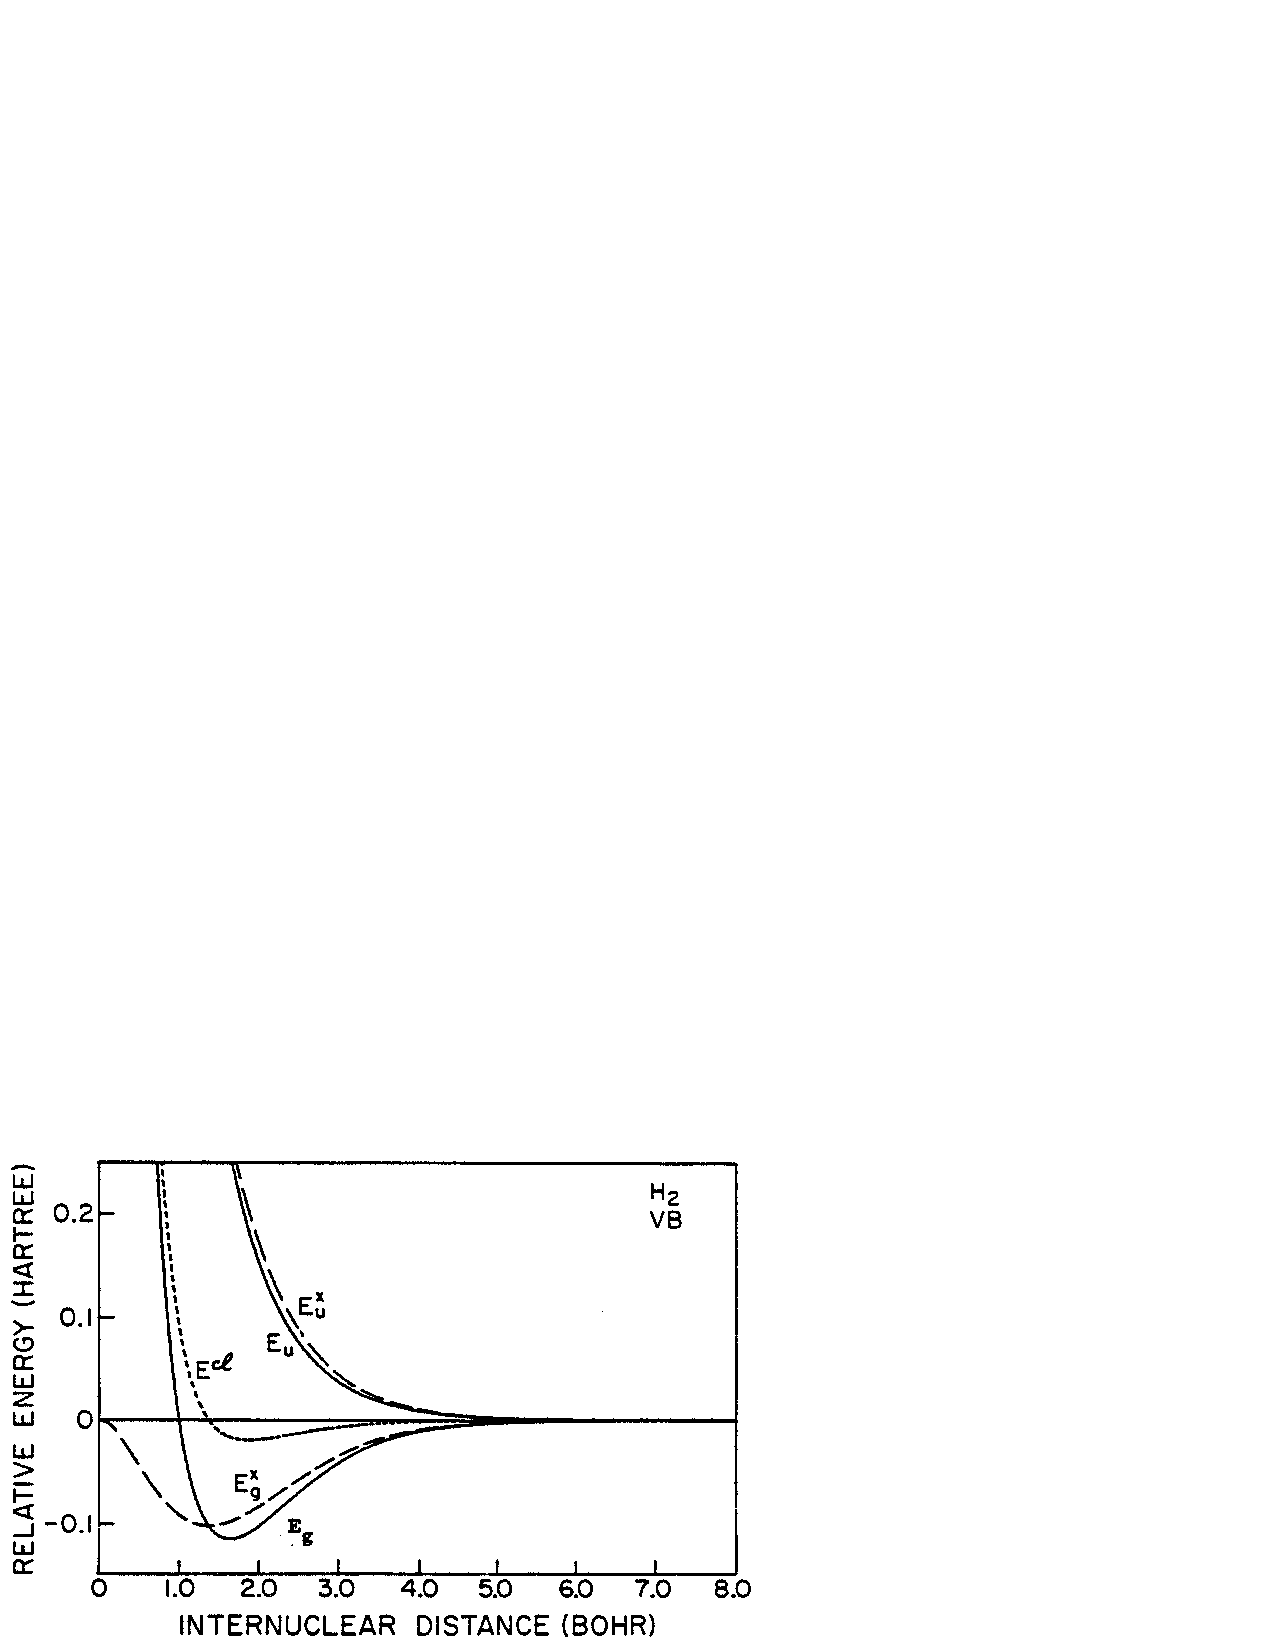
\includegraphics[scale=0.75]{fig2-30}
\caption{The classical ($E^{cl}$), exchange ($E^x$), and total ($E$)
  energies for the VB wave functions of H$_2$. Note that each energy
  is referenced to the value for $R = \infty$, that is,
  $E^{cl}(\infty) = E_g(\infty) = E_u(\infty) = -1.0$ and
  $E_g^x(\infty) = E_u^x(\infty) = 0.0$.}
\label{fig2-30}
\end{figure}

 
\subsubsection{Analysis of $E^{cl}$}

At large $R$, the one-electron term
\begin{equation}
h_{ll} = \underbrace{\langle \chi_\ell \vert - {1 \over 2} \nabla^2 - 
{1 \over r_a} \vert \chi_1 \rangle}_{{\rm atomic ~ energy}} + 
\underbrace{\langle \chi_\ell \vert - {1 \over r_b} \vert \chi_\ell 
\rangle}_{{\rm penetration ~ term}} ,
\end{equation}
has the form
\begin{equation}
h_{ll} \approx \epsilon_{1s} - {1 \over R} .
\end{equation}
(neglecting terms of order $e^{-2R}$), and the Coulomb term has the
form
\begin{equation}
J_{lr} \sim {1 \over R}
\end{equation}
(neglecting terms of order $e^{-2R}$).  Thus, the classical term is
just twice the energy of an $H$ atom, $\epsilon_{1s}$, 
\begin{equation}
E^{cl} \approx 2\epsilon_{1s}
\end{equation}
(neglecting terms of order $e^{-2R}$), with no net Coulomb terms.
Including the additional penetration terms lead to
\begin{equation}
E^{cl} = 2 \epsilon_{1s} + \left[ {1 \over R} + {5 \over 8} + {3 \over 
4} R - {1 \over 6} R^2 \right] e^{-2R} ,
\end{equation}
corresponding to the interpenetration of the two atomic electron
clouds.  Although negative for $R > 1.4\ a_0$, this quantity is small,
as shown in Figure \ref{fig2-30}. Thus, the bonding of H$_2$ cannot be
explained as due to penetration of the charge clouds of two hydrogen
atoms.

\subsubsection{The Exchange Terms}

Now we consider the energy of $\Phi^{COV}_g$, (\ref{eqno2-39a}),
\begin{equation}
E_g = {\langle \Phi_g \vert {\hat H} \vert \Phi_g \rangle \over 
\langle \Phi_g \vert \Phi_g \rangle} .
\end{equation}
By symmetry
\begin{equation}
\langle \Phi_g \vert \Phi_g \rangle = \langle \chi_\ell \chi_r \vert 
\Phi_g \rangle + \langle \chi_r \chi_\ell \vert \Phi_g \rangle = 2 
\langle \chi_\ell \chi_r \vert \Phi_g \rangle
\end{equation}
and
\begin{equation}
\langle \Phi_g \vert {\hat H} \vert \Phi_g \rangle = \langle \chi_\ell 
\chi_r \vert {\hat H} \vert \Phi_g \rangle + \langle \chi_r \chi_\ell 
\vert {\hat H} \vert \Phi_g \rangle = 2 \langle \chi_\ell \chi_r \vert 
{\hat H} \vert \Phi_g \rangle .
\end{equation}
Hence,
\begin{equation}
E_g = {\langle \chi_\ell \chi_r \vert {\hat H} \vert \Phi_g \rangle 
\over \langle \chi_\ell \chi_r \vert \Phi_g \rangle}
\end{equation}
Evaluating the individual terms, we find
\begin{equation}
\langle \chi_\ell \chi_r \vert \Phi_g \rangle = 1 + \langle \chi_\ell 
\vert \chi_r \rangle \langle \chi_r \vert \chi_\ell \rangle = 1 + S^2
\end{equation}
and
\begin{equation}
\langle \chi_\ell \chi_r \vert {\hat H} \vert \Phi_g \rangle = \langle 
\chi_\ell \chi_r \vert {\hat H} \vert \chi_\ell \chi_r \rangle + \langle 
\chi_\ell \chi_r \vert {\hat H} \vert \chi_r \chi_\ell \rangle = E^{cl} + 
{\cal E},
\end{equation}
where
\begin{equation}
{\cal E} = \langle \chi_\ell \chi_r \vert {\hat H} \chi_r \chi_\ell 
\rangle
\label{eqno2-44}
\end{equation}
is referred to as the \emph{valence bond exchange term}. Thus,
\begin{equation}
E_g = {E^{cl} + {\cal E} \over 1 + S^2} = E^{cl} + E^x_g ,
\end{equation}
where the exchange energy is
\begin{equation}
E^x_g = {\left( {\cal E} - S^2 E^{cl} \right) \over \left( 1 + 
S^2 \right)} .
\end{equation}
   
The same analysis for the $\Phi^{VB}_u$ wavefunction (\ref{eqno2-39b})
leads to
\begin{equation}
E_u = {E^{cl} - {\cal E} \over 1 - S^2} = E^{cl} + E^x_u ,
\end{equation}
where
\begin{equation}
E^x_u = - {\left( {\cal E} - S^2 E^{cl} \right) \over ( 1 - S^2 )} .
\end{equation}

The close relationship between $E_g^x$ and $E_u^x$ is emphasized by defining
\begin{equation}
{\bar{\tau}} = \left( {\cal E} - S^2 E^{cl} \right)
\label{eqno2-45}
\end{equation}
so that
\begin{equation}
E^x_g = {{\bar{\tau}} \over \left( 1 + S^2 \right)}
\label{eqno2-46}
\end{equation}
\begin{equation}
E^x_u = {- {\bar{\tau}} \over \left( 1 - S^2 \right)} .
\label{eqno2-47}
\end{equation}
We use ${\bar{\tau}}$ here in order to distinguish this quantity for
H$_2$ from the $\tau$ of H$^+_2$.  From equations (\ref{eqno2-46}) and
(\ref{eqno2-47}), the energy separation between the $g$ and $u$ states
is
\begin{equation}
E_g - E_u = {2 {\bar{\tau}} \over 1 - S^4}.
\label{eqno2-48}
\end{equation}
From the nodal theorem, $E_g < E_u$, and hence, ${\bar{\tau}} < 0$ since 
$S < 1$.
    
These results for H$_2$ are quite analogous to the case of H$^+_2$ where the
$\varphi_g$ and $\varphi_u$ state have energies
\begin{equation}
\epsilon_g = \epsilon^{cl} + \left[ {1 \over 1+S} \right]\tau
\end{equation}
\begin{equation}
\epsilon_u = \epsilon^{cl} - \left[ {1 \over 1-S} \right]\tau
\end{equation}
\begin{equation}
\epsilon_g - \epsilon_u = {2 \tau \over ( 1 - S^2)} ,
\end{equation}
with
\begin{equation}
\epsilon^{cl} = h_{ll} + {1 \over R}
\label{eqno2-49}
\end{equation}
\begin{equation}
\tau = h_{lr} - Sh_{ll}.
\end{equation}

\subsubsection{Analysis of ${\cal E}$}

The components of ${\cal E}$ (\ref{eqno2-44}) are
\begin{equation}
\langle \chi_\ell \chi_r \vert h ( 1 ) \vert \chi_r \chi_\ell \rangle = 
\langle \chi_\ell \vert h \vert \chi_r \rangle \langle \chi_r \vert 
\chi_\ell \rangle = h_{lr}S
\end{equation}
\begin{equation}
\langle \chi_\ell \chi_r \vert h (2) \vert \chi_r \chi_\ell \rangle = \langle 
\chi_\ell \vert \chi_r \rangle \langle \chi_r \vert h \vert \chi_\ell 
\rangle = S h_{rl}
\end{equation}
\begin{equation}
\langle \chi_\ell \chi_r \vert {1 \over r_{12}} \vert \chi_r \chi_\ell
\rangle = \int d \tau \chi^*_\ell (1)\chi_r(1) \int d \tau_2 {1 \over
r_{12}} \chi^*_r (2) \chi_\ell (2) = K_{lr}
\end{equation}
\begin{equation}
\langle \chi_\ell \chi_r \vert {1 \over R} \vert \chi_r \chi_\ell
\rangle = {S^2 \over R} ,
\end{equation}
where $S$ is the overlap and $K_{lr}$ is referred to as an exchange 
integral. Note the distinction between ${\cal E}$, the VB
exchange term, and $K_{1r}$, the exchange integral. Thus,
\begin{equation}
{\cal E} = 2 S h_{lr} + K_{lr} + {S^2 \over R} .
\end{equation}

\subsubsection{Analysis of ${\bar{\tau}}$}

\begin{figure}
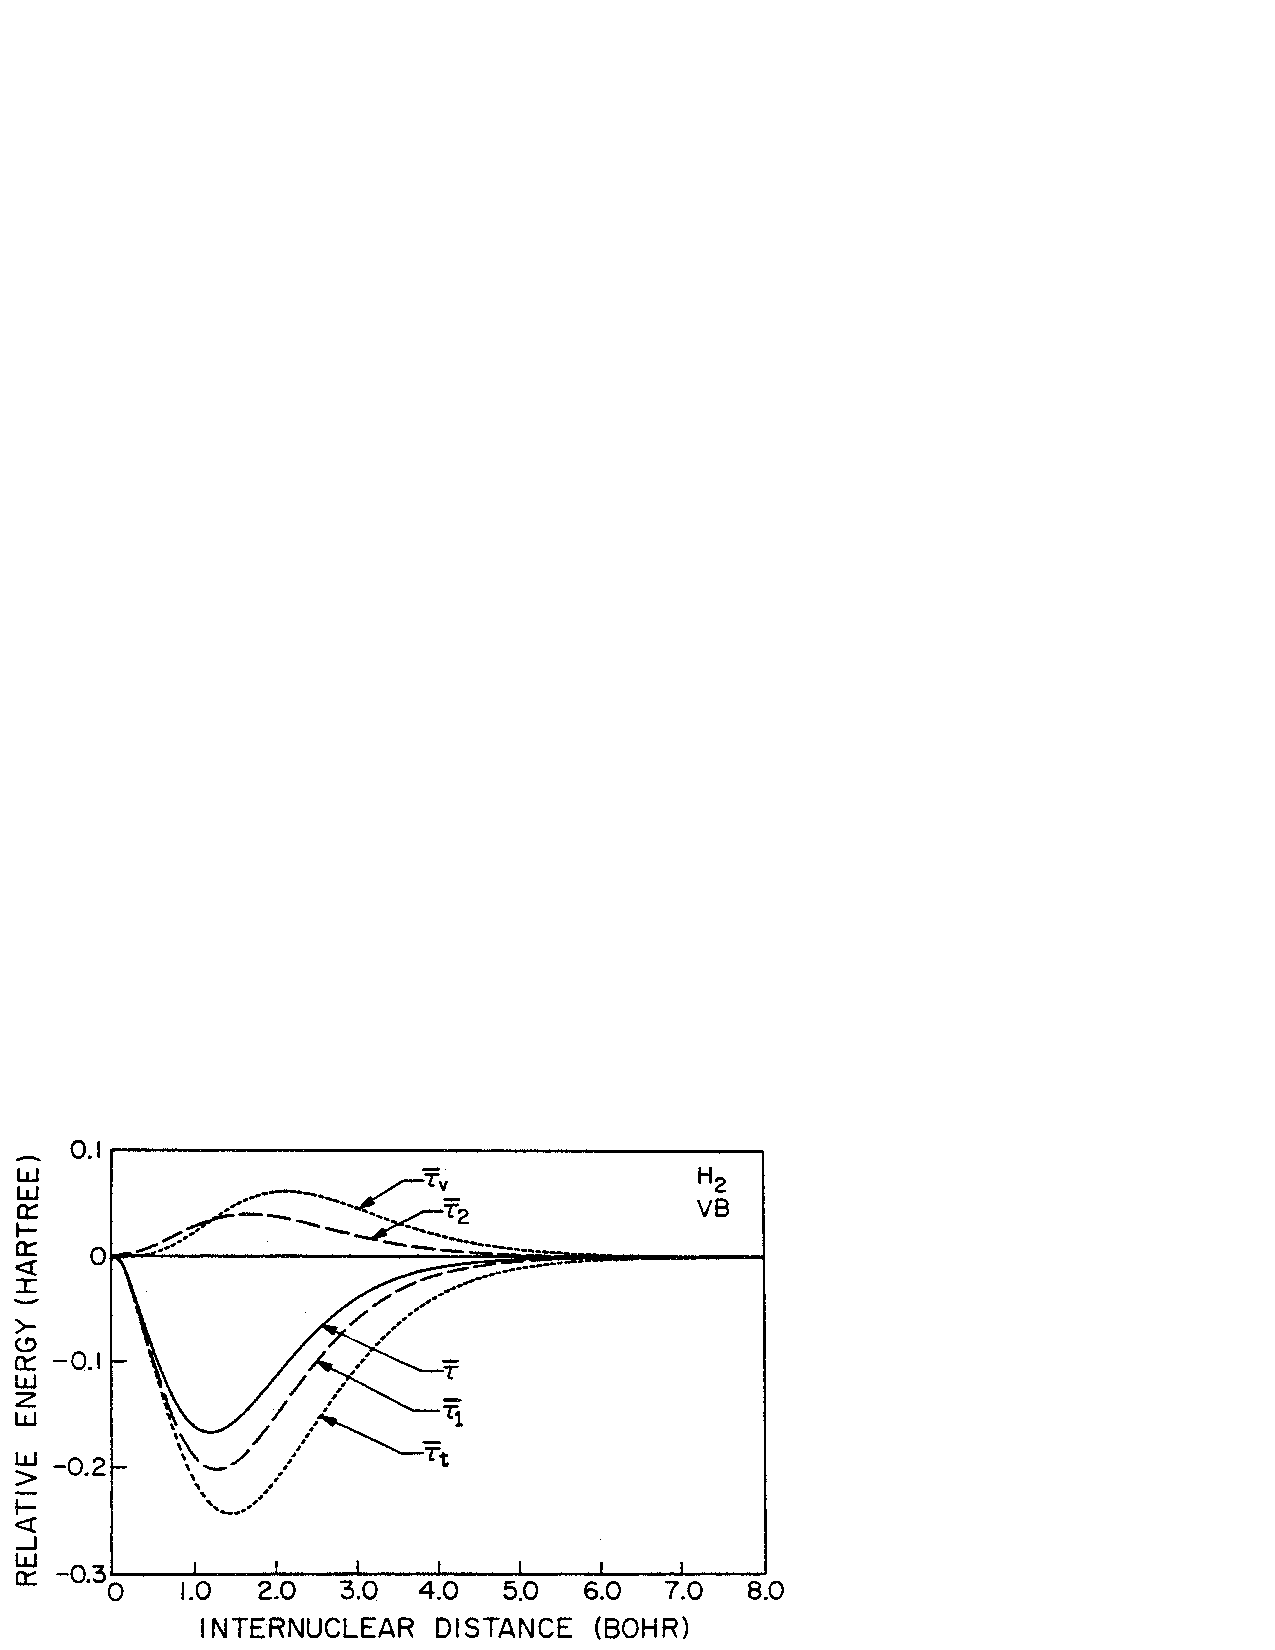
\includegraphics[scale=0.75]{fig2-31}
\caption{The total exchange term ($\bar{\tau}$) and the one-electron
  ($\bar{\tau}_1$) and two-electron ($\bar{\tau}_2$)
  parts. The potential ($\bar{\tau}_v$) and kinetic ($\bar{\tau}_t$)
  parts of $\bar{\tau}_1$ are also shown separately. All results are
  for H$_2$.}
\label{fig2-31}
\end{figure}

Using $E^{cl}$ from equation (\ref{eqno2-43}) in (\ref{eqno2-45}), we
find that ${\bar{\tau}} = {\bar{\tau}}_1 + {\bar{\tau}}_2$, where
\begin{equation}
{\bar{\tau}}_1 = \left[ 2 S h_{lr} - S^2 \left( h_{ll} + h_{rr} 
\right) \right] = 2S \left[ h_{lr} - S h_{ll} \right] = 2S \tau
\end{equation}
\begin{equation}
{\bar{\tau}}_2 = \left[ K_{lr} - S^2 J_{lr} \right]
\end{equation}
are the one- and two-electron parts, respectively (the $1/R$ terms
cancel). These quantities are plotted in Figure \ref{fig2-31}, where
we see that ${\bar{\tau}}_2$ has a smaller magnitude than
${\bar{\tau}}_1$.  Thus, ${\bar{\tau}} \approx {\bar{\tau}}_1$.  
Comparing equations (\ref{eqno-48}) and (\ref{eqno-49}), we see that
\begin{equation}
{\bar{\tau}} = 2S \tau.
\end{equation}
That is, the one-electron part of
${\bar{\tau}}$ for H$_2$ is related directly to the $\tau$ of H$^+_2$,
leading to
\begin{equation}
{\bar{\tau}} \approx {\bar{\tau}}_1 - 2S \tau ,
\end{equation}
where $\tau$ is the quantity for H$^+_2$.  Thus, for H$_2$ the bonding 
energy is determined by
\begin{equation}
E^x_g \approx {2S \tau \over 1 + S^2} = {\bar{E}}^x_g
\label{eqno2-50}
\end{equation}
\begin{equation}
E^x_u \approx - {2S \tau \over 1 - S^2} = {\bar{E}}^x_u
\label{eqno2-51}
\end{equation}
whereas for H$^+_2$ it is determined by
\begin{equation}
\epsilon^x_g = {\tau \over 1+S}
\label{eqno2-52}
\end{equation}
\begin{equation}
\epsilon^x_u = - {\tau \over 1 - S}.
\label{eqno2-53}
\end{equation}
These quantities are compared in Figure \ref{fig2-32}.

\begin{figure}
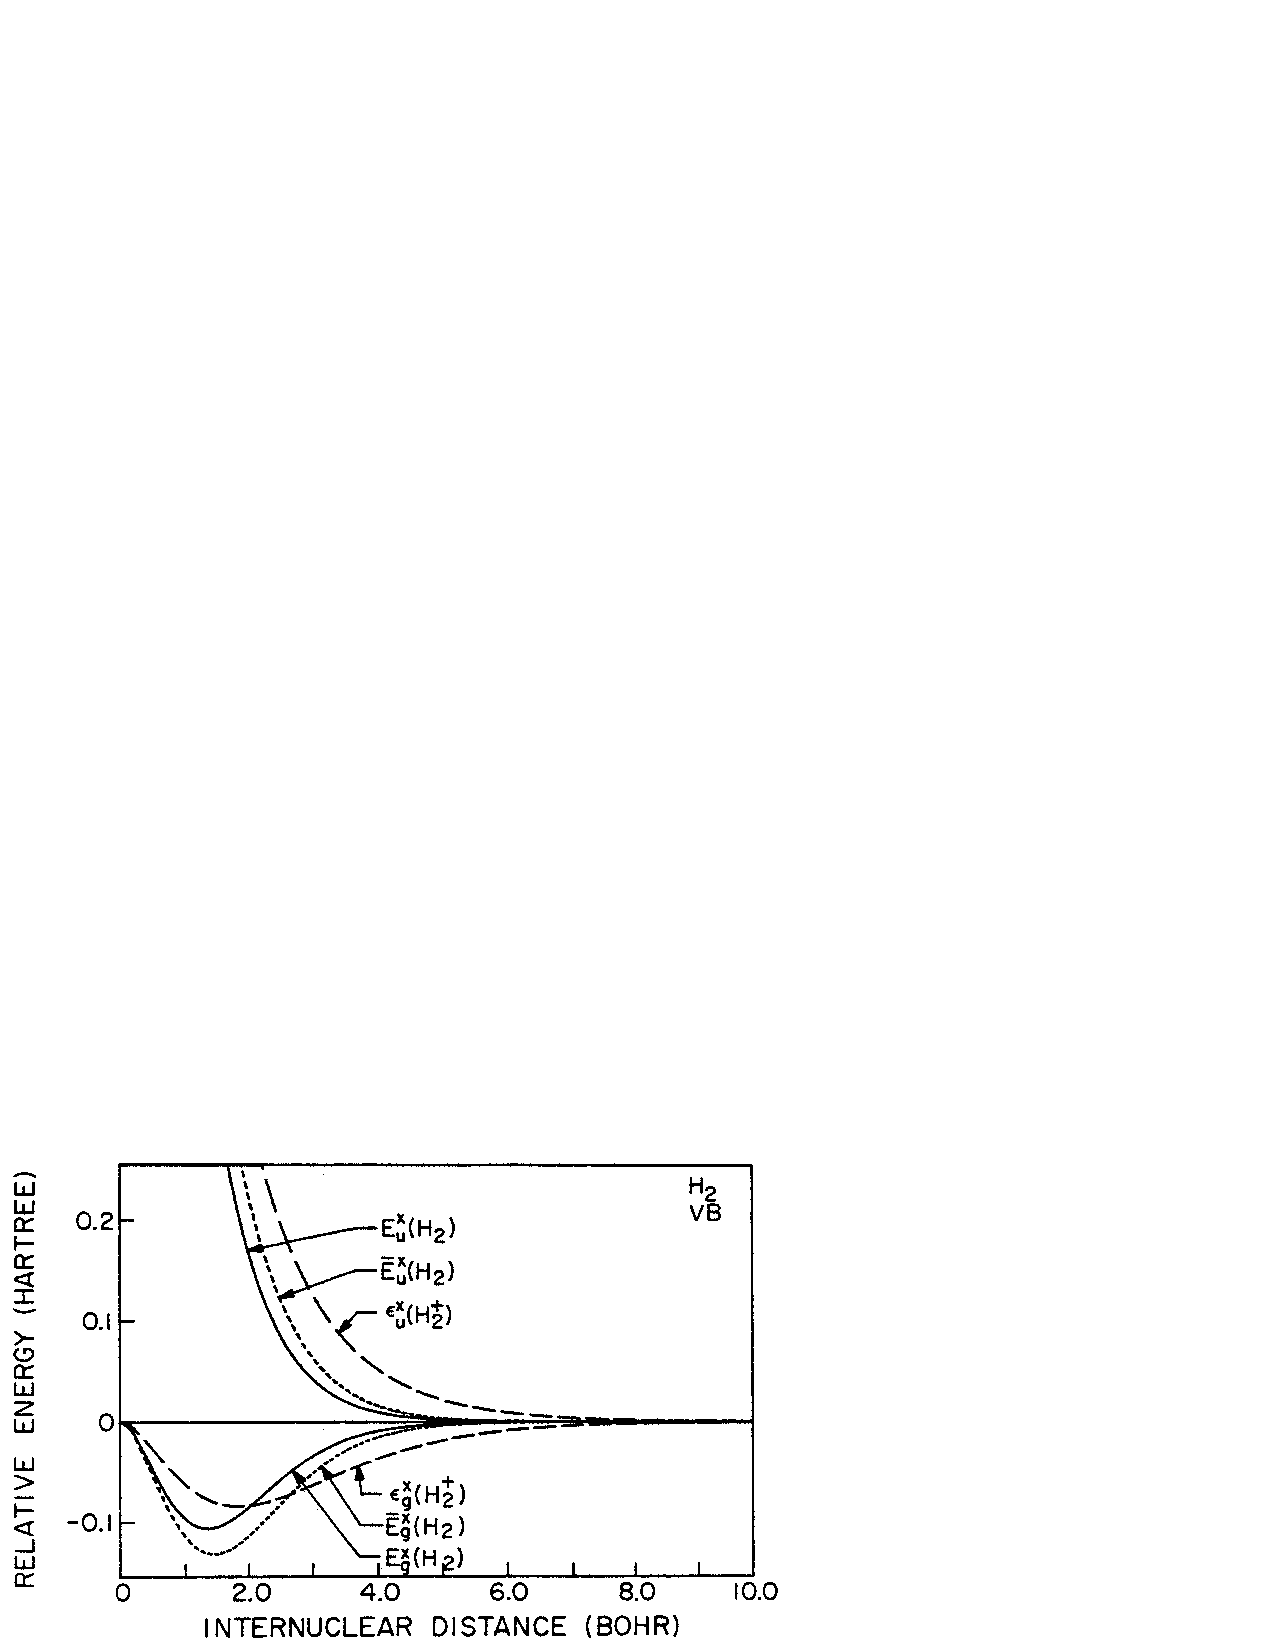
\includegraphics[scale=0.75]{fig2-32}
\caption{The exchange energies ($E_g^x$ and $E_u^x$) for H$_2^+$ and
  H$_2$. In addition, the one-electron approximation $\bar{E}^x$ to
  the $E^x$ for H$_2$ is shown for each state.}
\label{fig2-32}
\end{figure}

\subsubsection{Analysis of ${\bar{\tau}}+1 = 2S \tau$}

\begin{figure}
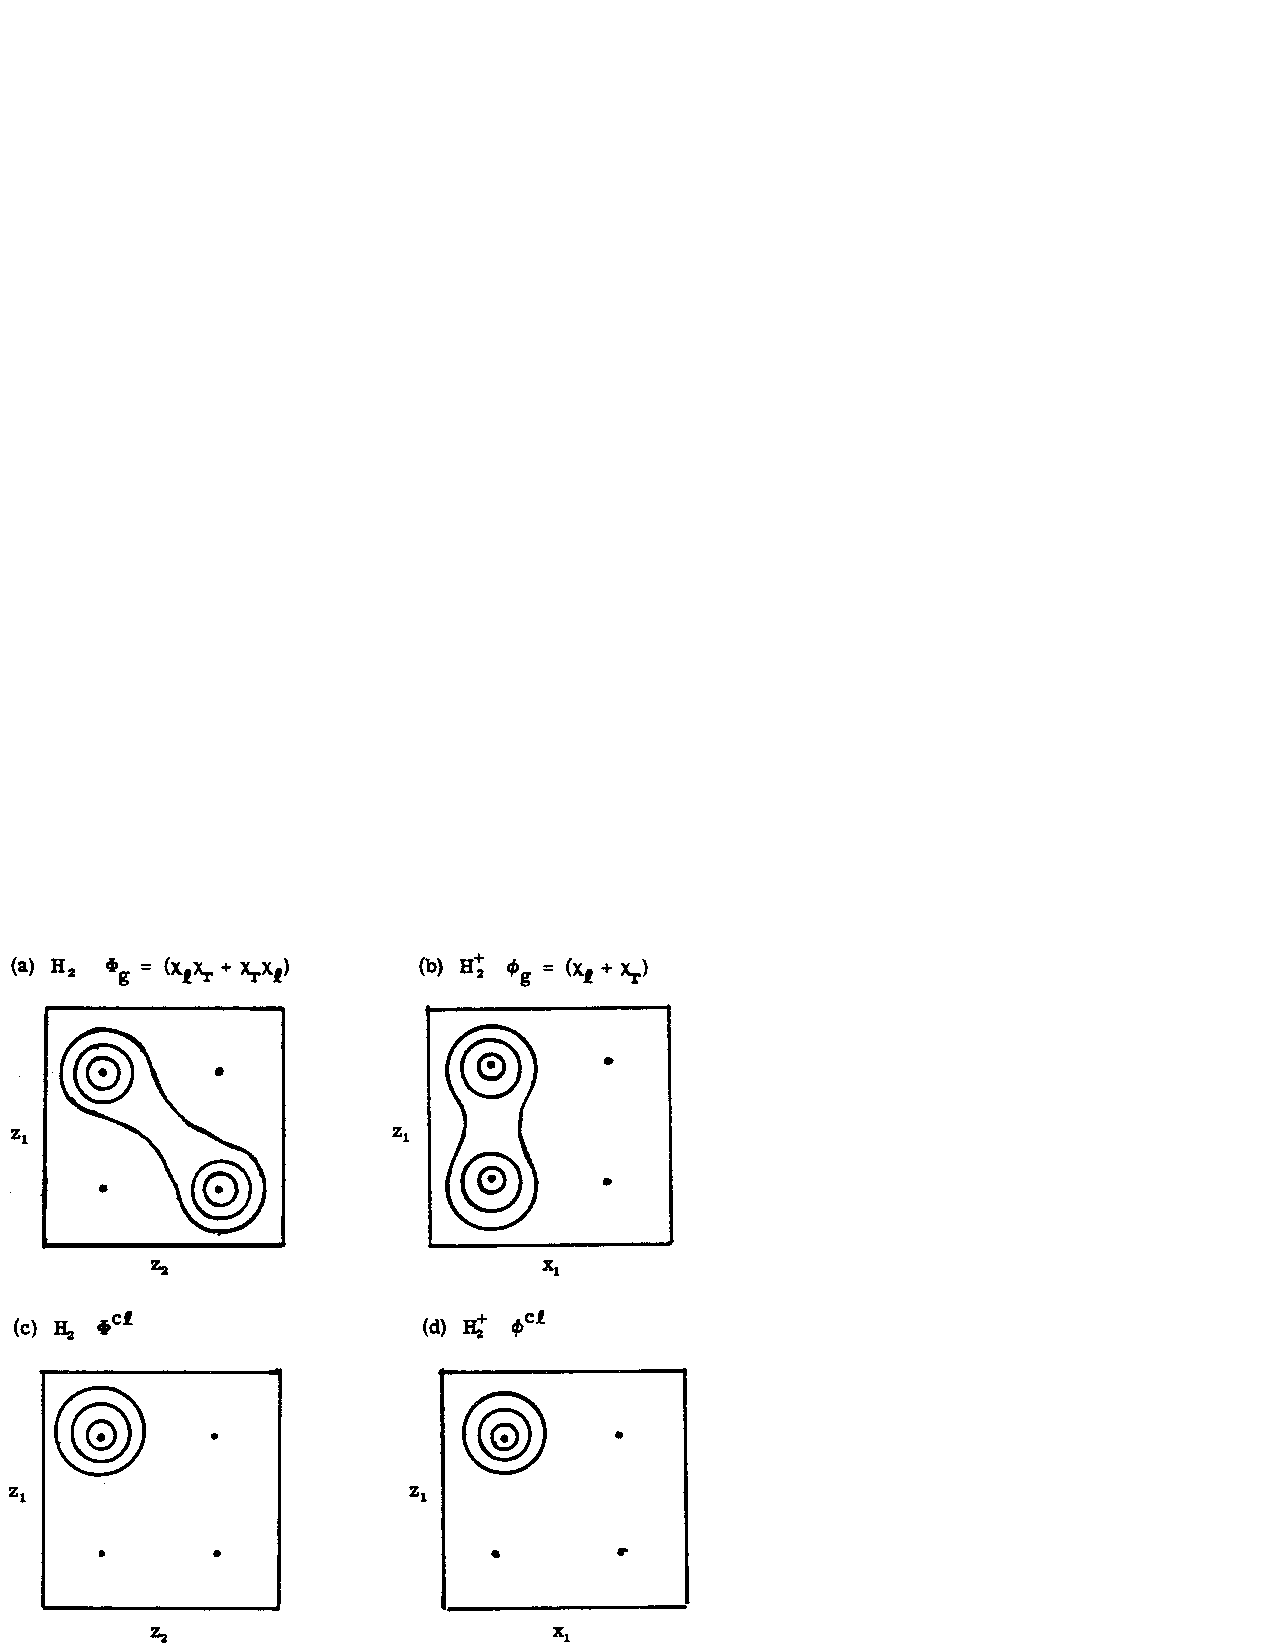
\includegraphics[scale=0.75]{fig2-33}
\caption{(a) H$_2$. $\Phi_g = (\chi_\ell \chi_r + \chi_r \chi_\ell)$;
(b) H$^+_2$, $\varphi_g = \phi_g = ( \chi_\ell + \chi_r)$;
(c) H$_2$, $\Phi^{cl}$; (d) H$^+_2$, $\varphi^{cl}$}
\label{fig2-33}
\end{figure}

Since the quantities ${\bar{\tau}}_1$ and $\tau$ dominating the
bonding in H$_2$ and H$_2^+$ are related, 
\begin{equation}
{\bar{\tau}}_1 = 2S\tau,
\end{equation}
it is well to examine the reasons for these relations. The
wavefunctions for the bonding states of H$_2$ and H$^+_2$ are sketched
in Figures \ref{fig2-33}(a) and \ref{fig2-33}(b). In both cases, the
kinetic energy is decreased from that in the classical wavefunctions,
Figures \ref{fig2-33}(c) and \ref{fig2-33}(d).  The decrease in the
kinetic energy for electron 1 is obtained by examining the gradients
in the vertical direction (ordinate) of Figure \ref{fig2-33}. Here we
see that H$^+_2$ leads to larger decrease than H$_2$. Thus, the
combination is $S \tau$ for H$_2$, but $\tau$ for H$^+_2$.  However,
for H$_2$ there is a second electron (number 2) that has a similar
decrease. Thus, for H$_2$ the net is $2S \tau$ as compared to $\tau$
for H$^+_2$.

\subsubsection{Comparison of Bonding in H$_2$ and H$^+_2$}

Although the bonding energies of H$_2$ and H$^+_2$ are both determined
by $\tau$, we see from (\ref{eqno2-50}) to (\ref{eqno2-53}) that the
value of the overlap $S$ also plays an important role. From an earlier
section, the form of $\tau$ at large $R$ is
\begin{equation}
\tau \approx - \left( {2 \over R} \right) S,
\end{equation}
hence,
\begin{equation}
{\bar{\tau}}_1 = 2 S \tau \approx - \left( {4 \over R} \right) S^2.
\end{equation}
Thus, the bonding in H$^+_2$ is proportional to $S$, but the bonding in 
H$_2$ is proportional to the square of $S$.
    
At $R = 1.6\ a_0$, the value of $S$ is $S = 0.7$, and hence, for H$_2$, 
$E^x_g  = 0.94 \tau$ and $E^x_u = - 2.75 \tau$.  For H$^+_2$, 
$\epsilon^x_g = 0.67 \tau$ and $\epsilon^x_u = - 3.33 \tau$.  Thus, the $g$ 
state of H$_2$ should have a bond energy about 50\% larger than the 
$g$ state of H$^+_2$, while the $u$ state of H$_2$ should be 17\% less 
repulsive than the $u$ state of H$^+_2$.  In addition, we see that 
the $u$ state of H$_2$ should be about three times as
repulsive as the $g$ state is attractive.

At $R = 3\ a_0$, the overlap is $S = 0.1$, and hence, we obtain for 
H$_2$, $E^x_g = 0.20 \tau$ and $E^x_u = - 0.20 \tau$.  For H$^+_2$, 
$\epsilon^x_g = 0.91 \tau$ and $\epsilon^x_u = - 1.11 \tau$. Thus,
are this large $R$, the $g$ and $u$ states of H$^+_2$ are five times 
as attractive, or repulsive, as the $g$ and $u$ states of H$_2$. That 
is, at large $R$, the one-electron bond is much stronger than the 
two-electron bond. This difference is relative bond strengths of H$_2$ 
and H$^+_2$ for small, and large $R$ just results from the
overlap term S, that automatically arises in the exchange of a two-electron
wavefunction.
    
In the limit that $S = 1$, we have for H$_2$, $E^x_g = \tau$ and for 
H$^+_2$, $\epsilon^x_g = 1/2 \tau$, leading to an H$_2$ bond twice that 
of H$^+_2$, the commonly expected result.  Actually, $S = 1$ implies 
$R = 0$, which in turn implies $\tau = 0$.

\section{Appendices}
\subsection{Energy Quantities of H$^+_2$}
\label{appendix-a}
    
We will consider an atomic orbital of the form
\begin{equation}
\chi = \sqrt{{\zeta^3 \over \pi}} e^{- \zeta r}
\label{eqno2app-1}
\end{equation}
centered at each of the two nuclei of H$^+_2$. The coordinates are
indicated in Figure \ref{fig2app-1}.

\begin{figure}
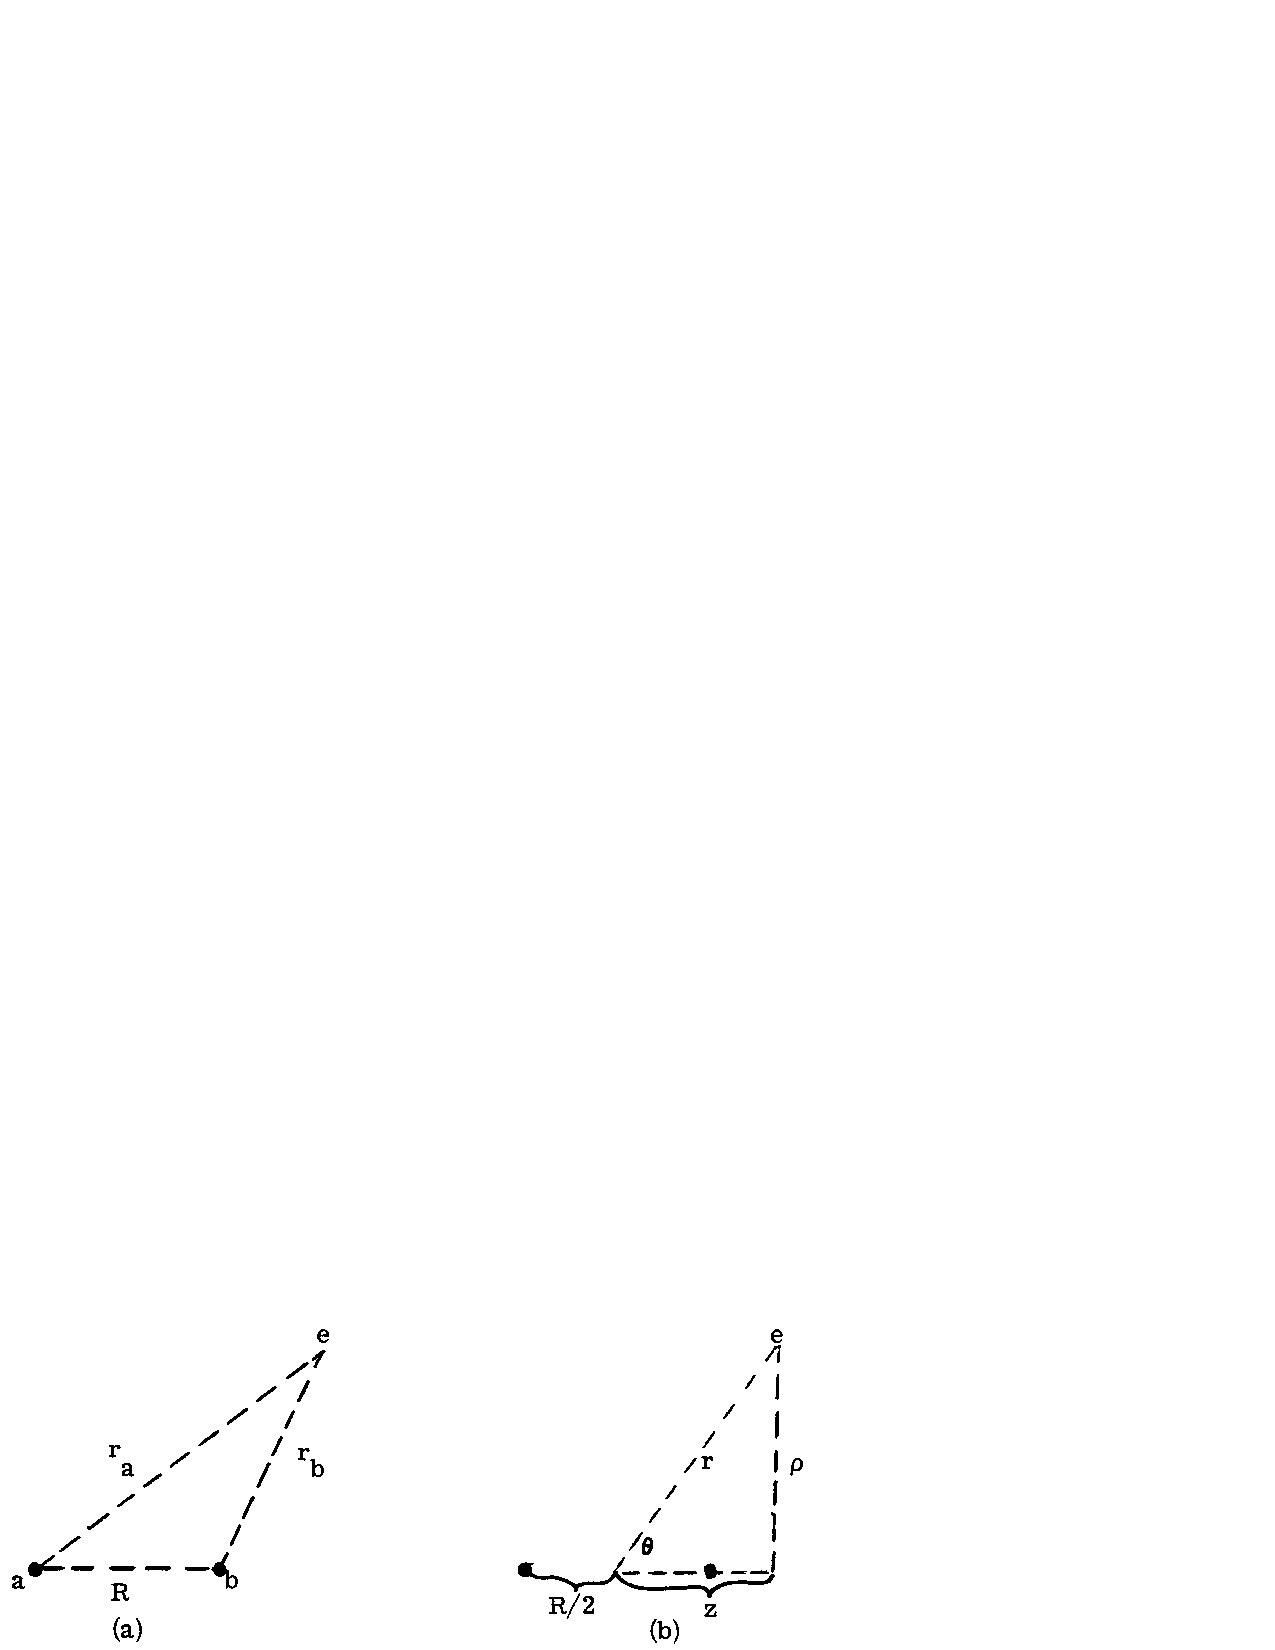
\includegraphics[scale=0.75]{fig2-34}
\caption{}
\label{fig2app-1}
\end{figure}

\noindent
With $\zeta = 1$, the orbitals (\ref{eqno2app-1}) correspond to
hydrogen $1s$ orbitals on each center. First, we evaluate the atomic
integrals for general $\zeta$, then the new energy quantities occuring
in H$^+_2$. First we consider the atomic energy quantities.

\subsubsection{Atomic Energy Quantities}

The norm of $\chi$ is
\begin{eqnarray}
\langle \chi \vert \chi \rangle &=& \left( {\zeta^3 \over \pi} \right) 
\int\limits^{\pi}_{0} \sin \theta d \theta \int\limits^{2 \pi}_{0}  
d \varphi \int\limits^{\infty}_{0} r^2 dr\ e^{-2 \zeta r}\cr
&=& 4 \zeta^3 \int\limits^{\infty}_{0} r^2 dre^{-2 \zeta r} = {1 \over 
2} \int\limits^{\infty}_{0} p^2 e^{-p} dp = 1,
\end{eqnarray}
where we set $p = 2 \zeta r$ and used
\begin{equation}
\int\limits^{\infty}_{0} p^m e^{-p} dp = m !.
\end{equation}

Similarly, the atomic potential energy is
\begin{equation}
\langle \chi \vert - {1 \over r} \vert \chi \rangle = - 4 \zeta^3 
\int\limits^{\infty}_{0} r^2 dr\ e^{-2 \zeta r} = - \zeta
\end{equation}
and the kinetic energy is
\begin{equation}
\langle \chi \vert - {1 \over 2} \nabla^2 \vert \chi \rangle = {1 
\over 2} \langle \vert \nabla \chi \vert^2 \rangle = {1 \over 2} 
\zeta^2 \langle \chi \vert \chi \rangle = {1 \over 2} \zeta^2.
\end{equation}

\subsubsection{Elliptic Coordinates}

In evaluating the energy quantities for diatomic molecules, it is convenient 
to use elliptic coordinates
\begin{equation}
\xi = {\left( r_a + r_b \right) \over R}
\label{eqno2app-2a}
\end{equation}
\begin{equation}
\eta = {\left( r_a - r_b \right) \over R}
\label{eqno2app-2b}
\end{equation}
and $\varphi$ equal to azimuthal angle about the $z$ axis, measured
from the $xz$ plane, in place of the cylindrical polar coordinate
$\rho$, $\varphi$, and $z$ or spherical coordinates $r$, $\theta$, and
$\varphi$, see Figure \ref{fig2app-1}(b). The geometric condition
defining an ellipse is that the sum of the distances to the two foci
is a constant. Hence, each curve of constant $\xi$ corresponds to an
ellipse. Similarly, from the defining condition of a hyperbola, each
surface of constant $\eta$ corresponds to a hyperbola. The range of
the elliptic coordinates is
\begin{equation}
0 \leq \xi < \infty
\end{equation}
\begin{equation} 
-1 \leq \eta \leq + 1
\end{equation}
\begin{equation}
0 \leq \varphi < 2 \pi
\end{equation}

The volume increments in the various coordinate systems are
\begin{eqnarray}
d \tau &=& dx\ dy\ dz\cr
d \tau &=& \rho\ d\rho\ d\varphi\ dz\cr
d \tau &=& r^2 \sin \theta\ dr\ d\theta\ d\varphi\cr
d \tau &=& {1 \over 8} R^3 \left( \xi^2 - \eta^2 \right) d\xi\ d\eta\ 
d\varphi
\label{eqno2app-3}
\end{eqnarray}
The latter relationship can be derived from
\begin{eqnarray*}
x &=& {1 \over 2} R \sqrt{\left( \xi^2 - 1 \right) \left( 1 - \eta^2 
\right)} \cos \varphi\cr
y &=& {1 \over 2} R \sqrt{\left( \xi^2 - 1 \right) \left( 1 - \eta^2 
\right)} \sin \varphi\cr
z &=& {1 \over 2} R \xi \eta\cr
\end{eqnarray*}
since the Jacobian ${1 \over 8} R^3 \left( \xi^2 - \eta^2 \right)$
is just the determinant of the derivative matrix.

From Figure \ref{fig2app-1}(b), we see that
\begin{eqnarray}
r^2_b &=& \rho^2 + \left( z - {R \over 2} \right)^2\cr
r^2_a &=& \rho^2 + \left( z + {R \over 2} \right)^2\cr
r^2 &=& \rho^2 + z^2,
\end{eqnarray}
and hence,
\begin{equation}
{1 \over 2} \left( r^2_a + r^2_b \right) = r^2 + \left( {R \over 2} 
\right)^2
\end{equation}
and
\begin{equation}
r^2_a - r^2_b = 2 z R.
\end{equation}
From (\ref{eqno2app-2a})--(\ref{eqno2app-2b}) we find
\begin{eqnarray}
{1 \over 2} \left( \xi^2 + \eta^2 \right) &=& {\left( r^2_a + r^2_b 
\right) \over R^2}\cr
\xi \eta &=& {\left( r^2_a - r^2_b \right) \over R^2}\cr
\xi^2 - \eta^2 &=& {4r_ar_b \over R^2}
\label{eqno2app-4}
\end{eqnarray}
and hence,
\begin{equation}
r^2 = {1 \over 4} R^2 \left[ \xi^2 + \eta^2 - 1 \right].
\label{eqno2app-5}
\end{equation}
These relations will be useful in the next section.

In evaluating integrals over $\xi$, the following integral will be useful
\begin{equation}
\int\limits^{\infty}_{x_0} x^m e^{- \alpha x} dx = {m!e^{- \alpha 
x_0} \over a^{m+1}} \sum^{m}_{k=0} {\left( ax_0 \right)^k \over k!} 
= A_m \left( \alpha x_0 \right)
\label{eqno2app-6}
\end{equation}
For $x_0 = 1$ and $m = 0$, 1, and 2, this becomes
\begin{equation}
A_0 ( \alpha ) = {1 \over \alpha} e^{- \alpha}
\label{eqno2app-7}
\end{equation}
\begin{equation}
A_1 ( \alpha ) = {1 \over \alpha^2} e^{- \alpha} \left[ 1 + \alpha 
\right]
\end{equation}
\begin{equation}
A_2 ( \alpha ) = {2 \over \alpha^3} e^{- \alpha}
\left[ 1 + \alpha + {1 \over 2} \alpha^2 \right]
\label{eqno2app-8}
\end{equation}

\subsubsection{Diatomic Energy Quantities}

First we evaluate the overlap integral,
\begin{equation}
S = \langle \chi_\ell \vert \chi_r \rangle .
\end{equation}
Using (\ref{eqno2app-1}), (\ref{eqno2app-3}), (\ref{eqno2app-7}) andqn
(\ref{eqno2app-8}), this becomes
\begin{eqnarray}
S = \int d \tau \chi_\ell \chi_r &=& \left( {\zeta^3 \over \pi} \right) 
\left( {R^3 \over 8} \right) ( 2 \pi ) \int\limits^{\infty}_{1} d 
\xi \int\limits^{+1}_{-1} d \eta \left( \xi^2 - \eta^2 \right) e^{-2 
\zeta R \xi}\cr
&=& e^{- \zeta r} \left[ 1 + ( \zeta R ) + {1 \over 3} ( \zeta R )^2 
\right]
\label{eqno2app-9}
\end{eqnarray}

There are two terms involved in evaluating the potential energy of 
H$^+_2$, the  exchange terms
\begin{equation}
V_{lr} = \langle \chi_\ell \vert {\hat v} \vert \chi_r \rangle ,
\end{equation}
where
\begin{equation}
{\hat v} = - {1 \over r_a} - {1 \over r_b}
\end{equation}
and
\begin{equation}
V_{ll} = \langle \chi_\ell \vert {\hat{v}} \vert \chi_\ell \rangle .
\end{equation}
In this section, we evaluate $V_{lr}$.
    
First we convert ${\hat{v}}$ to elliptic coordinates
\begin{equation}
{\hat v} = - {\left( r_a + r_b \right) \over r_ar_b} = - {4 \xi \over 
R \left( \xi^2 - \eta^2 \right)}
\label{eqno2app-10}
\end{equation}
using (\ref{eqno2app-2a})--(\ref{eqno2app-4}). Combining 
(\ref{eqno2app-10}) with (\ref{eqno2app-3}) leads to
\begin{equation}
{\hat v} d \tau = - {1 \over 2} R^2 \xi d \xi d \eta d \varphi ,
\end{equation}
and integrating over $\varphi$, we obtain
\begin{equation}
V_{lr} = \left( - {R^2 \over 2} \right) \left( {\zeta^3 \over \pi} 
\right) ( 2 \pi ) \int^{\infty}_{1} \xi d\xi e^{- \zeta 
R \xi} \int\limits^{+1}_{-1} d \eta = - 2 \zeta e^{-\zeta R} \left( 
1 + \zeta R \right) .
\end{equation}
 
The other potential energy term $V_{ll}$ has two
parts
\begin{equation}
V_{ll} = \langle \chi_\ell \vert - {1 \over r_a} \vert \chi_\ell 
\rangle + \langle \chi_\ell \vert - {1 \over r_b} \vert \chi_\ell \rangle ,
\end{equation}
the first of which is
\begin{equation}
V_{ll}^{(1)} = \langle \chi_\ell \vert - {1 \over r_a} \vert \chi_\ell 
\rangle
\end{equation}
is a one center integral, involving only the left nucleus, and the other 
of which is
\begin{equation}
V_{ll}^{(2)} = \langle \chi_\ell \vert - {1 \over r_b} \vert \chi_\ell 
\rangle
\end{equation}
involves two centers. This second term is the Coulomb interaction between
the spherically symmetric charge distribution $\rho_\ell - \vert \chi_\ell 
\vert^2$, centered on the left nucleus
with the charge centered on the right nucleus and is referred to as
the \emph{penetration integral}.
    
As shown below,
\begin{equation}
V_{ll}^{(2)} = A + B ,
\end{equation}
where
\begin{equation}
A = - {Q \over R}
\end{equation}
\begin{equation}
B = - 4 \pi \left( {\zeta^3 \over \pi} \right) \int\limits^{\infty}_{R} r_a 
dr_a e^{-2 \zeta r_a} 
\end{equation}
and
\begin{equation}
Q = 4 \pi \left( {\zeta^3 \over \pi} \right) \int\limits^{R}_{0} r^2_a 
dr_a e^{-2 \eta r_a} .
\end{equation}
Using
\begin{equation}
\int\limits^{R}_{0} r^2_a dr\ e^{- \alpha r} = {2 \over \alpha^3} 
\left[ 1 - \left( 1 + \alpha R + {1 \over 2} \alpha^2 R^2 \right) 
e^{- \alpha R} \right] ,
\end{equation}
we obtain
\begin{equation}
Q = \left[ 1 - \left( 1 + 2 \zeta R + 2 \zeta^2 R^2 \right) e^{- 2 
\zeta R} \right] .
\end{equation}
Using (\ref{eqno2app-6}), we obtain
\begin{equation}
B = - \zeta e^{-2 \zeta R} \left( 1 + 2 \zeta R \right),
\end{equation}
and hence,
\begin{equation}
V_{ll}^{(2)} = - {1 \over R} \left( 1 - e^{-2 \zeta R} \right) + 
\zeta e^{-2 \zeta R} .
\end{equation}

The two-center kinetic energy integral is
\begin{equation}
t_{lr} = \langle \chi_\ell \vert - {1 \over 2} \nabla^2 \vert 
\chi_r \rangle ,
\end{equation}
which, from the Appendix in Chapter \ref{chap01}, becomes
\begin{equation}
t_{lr} = {1 \over 2} \langle \nabla \chi_\ell \cdot \nabla \chi_r 
\rangle = {1 \over 2} \int d \tau \left( \nabla \chi_\ell \cdot \nabla 
\chi_r \right).
\label{eqno2app-11}
\end{equation}
Since
\begin{equation}
r_b = \sqrt{x^2 + y^2 + \left( z-{R \over 2} \right)^2}
\end{equation}
\begin{equation}
r_a = \sqrt{x^2 + y^2 + \left( z+{R \over 2} \right)^2} ,
\end{equation}
we obtain
\begin{equation}
{\hat \nabla} e^{- \zeta r_a} = - {\zeta \over r_a} e^{- \zeta r_a} 
\left[ x {\hat e}_x + y {\hat e}_y + \left( z + {1 \over 2} R 
\right) {\hat e}_z \right]
\end{equation}
\begin{equation}
{\hat \nabla} e^{- \zeta r_b} = - {\zeta \over r_b} e^{- \zeta r_b} 
\left[ x {\hat e}_x + y {\hat e}_y + \left( z - {1 \over 2} R 
\right) {\hat e}_z \right]
\end{equation}
where ${\hat e}_x$ denotes a unit vector in the $x$ direction. Hence,
\begin{equation}
\left( \nabla e^{- \zeta r_a} \right) \cdot \left( \nabla e^{- \zeta 
r_b} \right) = \left( {\zeta^2 \over r_ar_b} \right) e^{- \zeta R 
\xi} \left[ x^2 + y^2 + \left( z^2 - {1 \over 4} R^2 \right) \right]
\end{equation}
Using (\ref{eqno2app-3}), (\ref{eqno2app-5}), and (\ref{eqno2app-4}),
we obtain
\begin{equation}
d \tau \left( \nabla \chi_\ell \cdot \nabla \chi_r \right) = \left( {R^3 
\over 8} \right) \left( {4 \zeta^2 \over R^2} \right) \left( {\zeta^3 
\over \pi} \right) \left( {R^2 \over 4} \right) e^{- \zeta R \xi} 
\left( \xi^2 + \eta^2 - 2 \right) d \zeta d \eta d \varphi .
\end{equation}
Integrating over $\varphi$, and substituting into (\ref{eqno2app-11}),
leads to
\begin{eqnarray}
t_{lr} &=& {1 \over 8} R^3 \zeta^5 \int\limits^{\infty}_{1} d \zeta 
e^{- \zeta R \xi} \int\limits^{+1}_{-1} d \eta \left( \zeta^2 + 
\eta^2 - 2 \right)\cr
&=& {1 \over 4} R^2 \zeta^5 
\int\limits^{\infty}_{1} \left( \zeta^2 - {5 \over 3} \right) e^{- 
\zeta R \xi} d \zeta\cr
&=& {1 \over 2} \zeta^2 e^{- \zeta R} \left[ 1 + 
\zeta R - {1 \over 3} \left( \zeta R \right)^2 \right].
\end{eqnarray}

\subsubsection{Summary}

Collecting together the quantities of the previous sections, we have
\begin{equation}
\chi = \sqrt{{\zeta^3 \over \pi}} e^{- \zeta r}
\end{equation}
\begin{equation}
t_{ll} = \langle \chi_\ell \vert t \vert \chi_\ell \rangle = {1 
\over 2} \zeta^2
\end{equation}
\begin{equation}
V^{(1)}_{ll} = \langle \chi_\ell \vert - {1 \over r_a} \vert \chi_\ell 
\rangle = - \zeta
\end{equation}
\begin{equation}
S = \langle \chi_\ell \vert \chi_r \rangle = e^{- \zeta R} \left[ 1 + 
\zeta R + {1 \over 3} \left( \zeta R \right)^2 \right]
\end{equation}
\begin{equation}
t_{lr} = \langle \chi_\ell \vert t \vert \chi_r \rangle = {1 \over 2} 
\zeta^2 e^{- \zeta R} \left[ 1 + \zeta R - {1 \over 3} 
\left( \zeta R \right)^2 \right]
\end{equation}
\begin{equation}
V_{lr} = \langle \chi_\ell \vert \left( - {1 \over r_a} - {1 \over r_b} 
\right) \vert \chi_r \rangle = - 2 \zeta e^{- \zeta R} \left( 1 + 
\zeta R \right)
\end{equation}
\begin{equation}
V_{ll}^{(2)} = - {1 \over R} \left[ 1 - \left( 1 + \zeta R \right) 
e^{- 1 \zeta R} \right]
\end{equation}

\subsubsection{Qualitative Examination of Diatomic Quantities}

The amplitude of $\chi_r$ evaluated at the left nucleus is
\begin{equation}
\chi_r (R)  = \sqrt{{\zeta^3 \over \pi}} e^{- \zeta R}
\end{equation}
while the amplitude of $\chi_\ell$ at the left nucleus is
\begin{equation}
\chi_\ell (0) = \sqrt{{\zeta^3 \over \pi}}
\end{equation}
Thus,
\begin{equation}
\chi_r (R) = e^{- \zeta R} \chi_\ell (0)
\end{equation}
If $\chi_\ell$ were highly concentrated about the left nucleus, the 
overlap would be given by
\begin{equation}
S = e^{- \zeta R}
\label{eqno2app-12}
\end{equation}
Comparing with the correct formula (\ref{eqno2app-9}), we see that the
approximate form (\ref{eqno2app-12}) has the correct exponential
behavior on $R$ but the numerical coefficient in (\ref{eqno2app-12})
is correct only for $R = 0$. Using $R = 2.0\ a_0$ and $\zeta = 1.0$ in
(\ref{eqno2app-9}), leads to a coefficient of 3.33, and using $R =
6.0\ a_0$ leads to a coefficient of 19.0, many times the value obtained
with (\ref{eqno2app-12}).

\subsection{The Legendre Expansion}
Consider a system such as in Figure \ref{fig2app-1}. It is often
necessary to convert expressions involving, say the distance of the
electron from nucleus $b$ over to a new expression, involving the
distance of the electron from nucleus $a$, as indicated in Figure
\ref{fig2app-2}.

\begin{figure}
\begin{center}
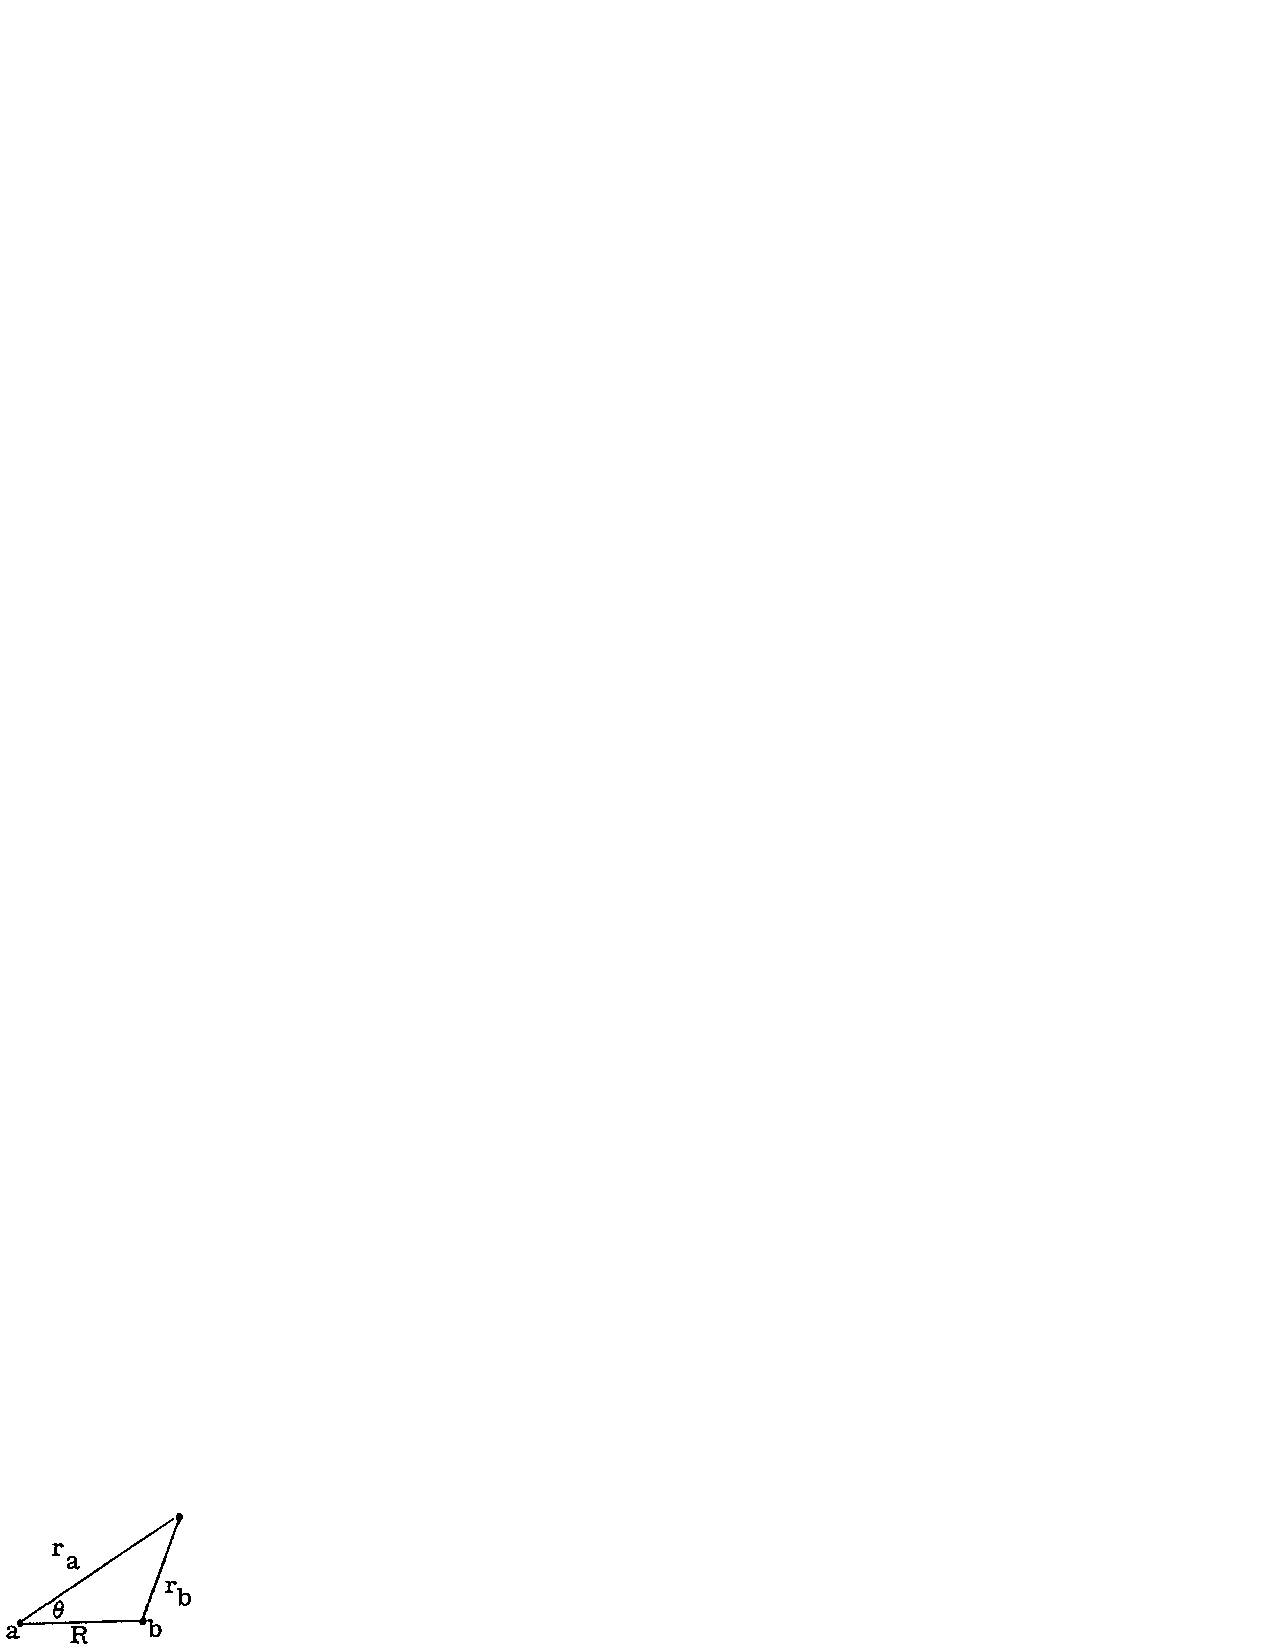
\includegraphics[scale=0.75]{fig2-35}
\end{center}
\caption{}
\label{fig2app-2}
\end{figure}

\noindent
The relation between these coordinates is
\begin{equation}
r^2_b = r^2_a + R^2 - 2 r_a R \cos \theta
\end{equation}
A case of particular importance, is to convert $1/r_b$ over to the new 
coordinates. This leads to
\begin{equation}
{1 \over r_b} = {1 \over r_a {\sqrt{1+ \rho^2 - 2 \rho \cos 
\theta}}}
\label{eqno2app-13}
\end{equation}
where $\rho = R / r_a$.  If $\rho < 1$, the radical in
(\ref{eqno2app-13}) can be expanded as
\begin{equation}
{1 \over {\sqrt{1 + \rho^2 - 2 \rho \cos \theta}}} = 
\sum^{\infty}_{l=0} \rho^l P_\ell ( \cos \theta ) ,
\end{equation}
where the $P_\ell ( \cos \theta )$ are the Legendre polynomials
\begin{equation}
P_0 \left( \cos \theta \right) = 1,
\end{equation}
\begin{equation}
P_1 ( \cos \theta ) = \sin \theta ,
\end{equation}
\begin{equation}
P_2 ( \cos \theta ) = {1 \over 2} \left( 3 \cos^2 \theta - 1 \right)
\end{equation}
etc. Thus (\ref{eqno2app-13}) becomes
\begin{equation}
{1 \over r_b} = \sum^{\infty}_{t=0} {(r_<)^t \over (r_>)^{l+1}} 
P_\ell ( \cos \theta ) ,
\end{equation}
where $r_<$ and $r_>$ denote the lesser and greater, respectively, 
of $r_a$ and $R$.
    
If there is a spherically symmetric charge distribution $\rho_a(r_a)$ 
centered at $a$, then the total electrostatic interaction with a 
charge centered at $b$ is
\begin{equation}
V = \int d \tau \rho_a (r_a) {1 \over r_b} = 2 \pi 
\sum^{\infty}_{t=0} \int\limits^{\infty}_{0} r^2_a d r_a \rho_a ( 
r_a ) \left[ {(r_<)^l \over (r_>)^{l+1}} \right] 
\int\limits^{\pi}_{0} \sin \theta d \theta P_\ell ( \cos \theta ),
\label{eqno2app-14}
\end{equation}
where we integrated over the $\varphi$ coordinate. The Lengendre 
polynomials have the property that
\begin{equation}
\int\limits^{\pi}_{0} \sin \theta d \theta P_\ell ( \cos \theta ) = 2 
\delta_{l0} ,
\end{equation}
so that (\ref{eqno2app-14}) becomes
\begin{equation}
V = 4 \pi \sum^{\infty}_{t=0} \int\limits^{\infty}_{0} r^2_a d r_a 
\rho_a ( r_a ) {1 \over r_>} = 4 \pi \left\{ {1 \over R} 
\int\limits^{R}_{0} r^2_a dr_a \rho_a ( r_a ) + 
\int\limits^{\infty}_{R} r_a dr_a \rho_a ( r_a ) \right\}.
\label{eqno2app-15}
\end{equation}
The quantity
\begin{equation}
Q = 4 \pi \int\limits^{R}_{0} r^2_a dr_a \rho_a ( r_a )
\end{equation}
is the amount of charge within the sphere centered at $a$ and passing 
through $b$. The contribution of this charge to $V$ is just the same as 
if all this charge were concentrated at $a$.

The quantity
\begin{equation}
\delta Q = 4 \pi r^2_a \rho_a ( r_a ) \delta r_a
\end{equation}
is the amount of charge on a sphere of radius $r_a$ and thickness 
$\delta r_a$.  The potential within such a uniformly charge sphere, is 
constant and equal to $1/r_a \delta Q$ as implied by the second
term of (\ref{eqno2app-15}).

\subsection{Coulomb and Exchange Integrals}
\label{appendix-b}

In the text, we indicated that
\begin{equation}
J_{ij} \geq K_{ij} \geq 0 .
\end{equation}
These relationships are now derived.

\subsubsection{$J_{ij}\geq 0$}

The Coulomb integral is
\begin{equation}
J_{ij} = \int d \tau_1 \varphi^*_i (1) \varphi_i(1) \int d \tau_2 {1 \over 
r_{12}} \varphi^*_j ((2) \varphi_j(2) = \int d \tau_1 d \tau_2 
{\varphi^*_i(1)\varphi_i(1)\varphi^*_j(2)\varphi_j(2) \over r_{12}} .
\end{equation}
Since the integrand is positive for all values of ${\bf r}_1$ and 
${\bf r}_2$, the integral must be positive. This integral is also denoted as
\begin{equation}
J_{ij} = \left[ \varphi^*_i \varphi_i \vert \varphi^*_j \varphi_j \right] ,
\end{equation}
where the orbitals on the left are for electron 1, and those on the 
right are for electron 2. This is often called \emph{chemist's
notation} for the two-electron integrals.

\subsubsection{$K_{ij} \geq 0$}

The exchange integral is
\begin{equation}
K_{ij} = \int d \tau_1 \varphi^*_i (1) \varphi_i(1) \int d \tau_2 {1 \over 
r_{12}} \varphi^*_j (2) \varphi_i(2) = \left[ \varphi^*_i \varphi_j \vert 
\varphi^*_j \varphi_i \right].
\end{equation}
To prove that $K_{ij} \geq 0$, we set
\begin{equation}
\varphi_i = \xi + i \eta_i
\end{equation}
\begin{equation}
\varphi_j = \xi_j + i \eta_j
\end{equation}
where $\xi_i$, $\eta_i$, $\xi_j$, and $\eta_j$ are real. This substitution 
leads to
\begin{eqnarray*}
K_{ij} &=& \left[ \left\{ \xi_i(1) - i \eta_i(1) \right\} \left\{ 
\xi_j(1) + i \eta_j(1) \right\} \vert \left\{ \xi_i(2) + i \eta_i(2) 
\right\} \left\{ \xi_j(2) - i \eta_j(2) \right\} \right]\cr
&=& \left\{ \xi_i \xi_j + \eta_i \eta_j + i \left( \xi_i \eta_j - 
\eta_i \xi_i \right) \vert \xi_i \xi_j + \eta_i \eta_j - i \left( 
\xi_i \eta_j - \eta_i \xi_j \right) \right].\cr
\end{eqnarray*}
We now define the charge distributions $\rho_1$ and $\rho_2$ as
\begin{equation}
\rho_1 = \xi_i \xi_j + \eta_i \eta_j
\end{equation}
\begin{equation}
\rho_2 = \xi_i \xi_j - \eta_i \eta_j .
\end{equation}
This leads to
\begin{equation}
K_{ij} = \left[ \rho_1 + i \rho_2 \vert \rho_1 - i \rho_2 \right] = 
\underbrace{\left[ \rho_1 \vert \rho_1 \right]}_{\geq 0} + 
\underbrace{i \left\{ \left[ \rho_2 \vert \rho_1 \right] - \left[ 
\rho_1 \vert \rho_2 \right] \right\}}_{=0} + 
\underbrace{\left[ \rho_2 \vert \rho_2 \right]}_{\geq 0} ,
\end{equation}
and hence, $K_{ij} \geq 0$.

\subsubsection{$J_{ij} \geq K_{ij}$}
  
To show that $J_{jj} \geq K_{ij}$, we consider the wavefunction
\begin{equation}
\Psi ( 1 , 2 ) = \varphi_i \varphi_j - \varphi_j \varphi_i
\end{equation}
The electron-electron interaction energy for this state is
\begin{equation}
\langle \Psi \vert {1 \over r_{12}} \vert \Psi \rangle = \int \int d 
\tau_1 d \tau_2 {1 \over r_{12}} \vert \psi (1,2) \vert^2 \geq 0 ,
\end{equation}
since the integrand is positive everywhere. Substituting the wavefunction 
from above leads to
\begin{equation}
\langle \Psi \vert {1 \over r_{12}} \vert \Psi \rangle = 2 \left( 
J_{ij} - K_{ij} \right)
\label{eqno2app-16}
\end{equation}
and hence, $J_{ij} \geq K_{ij}$.  Expression (16) provides the physical 
significance of $K_{ij}$.  It is the change in electron repulsion energy 
upon superimposing both products of orthogonal orbitals $\varphi_i 
\varphi_j$.  That is, wavefunctions
\begin{equation}
{1 \over \sqrt{2}} \left[ \varphi_i \varphi_j \pm \varphi_j \varphi_i \right]
\end{equation}
lead to Coulomb repulsion energies of $J_{ij} \pm K_{ij}$.

\subsection{Two-Electron Integrals of H$_2$}

\subsubsection{The Coulomb Integral}

The Coulomb integral, $J_{lr}$ has the form
\begin{equation}
J_{lr} = \langle \chi_\ell(1) \chi_\ell(1) \vert {1 \over r_{12}} \vert 
\chi_r(2) \chi_r(2) \rangle = \int d \tau_2 \left[ \int d \tau_2 
\chi^*_\ell (1) \chi_\ell (1) {1 \over r_{12}} \right] \chi^*_r(2) \chi_r(2)
\end{equation}
where $\chi_\ell$ and $\chi_r$ are $1s$ atomic orbitals centered on the 
left and right protons.  Letting
\begin{equation}
J_\ell(2) = \int d \tau_1 \chi^*_\ell (1) \chi_\ell (1) {1 \over r_{12}} ,
\end{equation}
we have
\begin{equation}
J_{lr} = \int d \tau_1 J_\ell (2) \chi^*_r (2) \chi_r (2) .
\label{eqno2app-17}
\end{equation}
In the remainder of this section, we will assume $\chi_\ell$ and
$\chi_r$ are real.
    
First we evaluate $J_\ell$ by expanding $1/r_{12}$ as
\begin{equation}
{1 \over r_{12}} = \sum^{\infty}_{k=0} \sum^{k}_{m=-k} {\left( k - 
\vert m \vert \right) ! r^k_< \over \left( k + \vert m \vert \right) ! 
r^{k+1}_>} P^{|m|}_k \left( \cos \theta_1 \right) P^{|m|}_k \left( 
\cos \theta_2 \right) e^{im(\varphi_1 - \varphi_2)}
\end{equation}
the Laplace expansion, where $r_{12}$ is the distance between the points 
with spherical coordinates $r_1$, $\theta_1$, and $\varphi_1$, and 
$r_2$, $\theta_2$, and $\varphi_2$.

Note that both $r_1$ and $r_2$ are with respect to the left-hand 
center. Since $\chi_\ell$ is spherically symmetric, about center $l$, the 
integrals over $\theta_1$  and $\theta_2$ will be nonzero only when $k = 
m = 0$
\begin{equation}
J_\ell = 4 \pi \int\limits^{\infty}_{0} r^2_{a1} d r_{a1} \chi^2_\ell 
\left( r_{a1} \right) {1 \over r_>} .
\end{equation}
Breaking the interval of integration to remove the $r_>$ yields,
\begin{equation}
J_\ell(2) = {1 \over r_{a2}} 4 \pi \left[ \int\limits^{r_{a2}}_{0} 
\chi^2_\ell \left( r_{a1} \right) r^2_{a1} d r_{a1} + 
\int\limits^{\infty}_{r_{a2}} \chi^2_\ell \left( r_{a1} \right) r_{a1} 
r_{a2} d r_{a1} \right]
\end{equation}
Letting
\begin{equation}
\chi_\ell(1) = \sqrt{{\zeta^3 \over \pi}} e^{- \zeta r_{a1}} ,
\end{equation}
we find
\begin{equation}
J_\ell \left( r_{a2} \right) = {1 \over r_{a2}} \left[ 1 - e^{-2 \zeta 
r_{a2}} \left( 1 + \zeta r_{a2} \right) \right]
\label{eqno2app-18}
\end{equation}
Now we must change to elliptic coordinates in order to evaluate the 
integral over the coordinates of electron 2.
    
Using elliptical coordinates $\xi$ and $\eta$,
\begin{equation}
\xi = {\left( r_a + r_b \right) \over R}
\end{equation}
\begin{equation}
\eta = {\left( r_a - r_b \right) \over R}
\end{equation}
\begin{equation}
d \tau = {R^3 \over 8} \left( \xi^2 - \eta^2 \right) d \xi d \eta d 
\varphi
\end{equation}
\noindent
in (\ref{eqno2app-18}) and (\ref{eqno2app-17}), we find
\begin{eqnarray*}
J_{lr} &=& {\xi^3 R^2 \over 4 \pi} \int\limits^{2 \pi}_{0} d \varphi 
\int\limits^{1}_{-1} d \eta \int\limits^{\infty}_{1} d \xi \left\{ 
\left( \xi^2 - \eta^2 \right) e^{- \zeta R(\xi - \eta)}\right.\cr
&& \left. \times {1 
\over ( \xi + \eta)} \left[ 1 - e^{- \zeta R(\xi + \eta)} \left( 1 + 
{\zeta \over 2} R \left( \xi + \eta \right) \right) \right] \right\}\cr
&=& {\zeta^3R^2 \over 2} \int\limits^{1}_{-1} d \eta 
\int\limits^{\infty}_{1} d \xi ( \xi - \eta) \left[ e^{- \zeta 
R(\xi-\eta)} - e^{-2\zeta R\xi} \left( 1 + {\zeta \over 2} R ( 
\zeta + \eta ) \right) \right]\cr
\end{eqnarray*}
or
\begin{eqnarray*}
J_{lr} &=& {\zeta^3R^2 \over 2} \int\limits^{1}_{-1} d \eta 
\int\limits^{\infty}_{1} d \xi ( \xi - \eta) e^{- \zeta 
R(\xi-\eta)}\cr
&+& {\zeta^3R^2 \over 2} \int\limits^{1}_{-1} d \eta 
\int\limits^{\infty}_{1} d \xi ( \xi - \eta) e^{- 2 \zeta R \xi} + 
{\zeta^4R^3 \over 2} \int\limits^{1}_{-1} d \eta 
\int\limits^{\infty}_{1} d \xi ( \xi^2 - \eta^2)
e^{- 2 \zeta R \xi}\cr
\end{eqnarray*}

Evaluating these elementary integrals, gives the following result
\begin{equation}
J_{lr} = \zeta \left[ {1 \over \zeta R} - e^{-2 \zeta R} \left( {1 
\over \zeta R} + {11 \over 8} + {3 \over 4} \zeta R + {1 \over 6} 
\zeta^2 R^2 \right) \right]
\end{equation}

\subsubsection{The Exchange Integral}

Now we evaluate the exchange integral
\begin{equation}
K_{lr} = \langle \chi_\ell ( 1 ) \chi_r ( 2 ) \vert {1 \over r_{12}} 
\vert \chi_r ( 1 ) \chi_\ell ( 2 ) \rangle = \left[ \chi_\ell \chi_r \vert 
\chi_\ell \chi_r \right] .
\end{equation}
Again, we can define a quantity
\begin{equation}
I(2)  = \int d \tau_1 \left[ \chi_\ell ( 1 ) \chi_r ( 1 ) {1 \over 
r_{12}} \right]
\end{equation}
involving integration over the first electron.  Unfortunately, the 
Laplace expansion of $1/r_{12}$ will now lead to an infinite sum 
because $\chi_\ell(1)\chi_r(1)$ is not spherically symmetric.
    
Instead, we expand $1/r_{12}$ in terms of elliptical coordinates 
using the Neuman expansion,
\begin{eqnarray*}
{1 \over r_{12}} &= & {2 \over R} \sum^{\infty}_{k=0} \sum^{k}_{m=-k} 
\left( - 1 \right)^m \left( 2 k + 1 \right) \left[ {(k-|m|)! \over 
(k+|m|)!} \right]^2\cr
& &\times P^{|m|}_k \left[ \xi_< \right] 
Q^{|m|}_k [\xi_>] P^{|m|}_k (\eta_1) P^{|m|}_k (\eta_2) 
e^{im(\varphi_1 - \varphi_2)}\cr
\end{eqnarray*}
where $P^{|m|}_k$ are the associated Legendre functions, and 
$Q^{|m|}_k$ are the associated Legendre functions of the second kind.
    
Our function $\chi_\ell\chi_r$ is independent of $\varphi$ so the only 
nonzero term in the $m$ summation is $m = 0$. To simplify the $k$ 
summation, we use the property
\begin{equation}
\int\limits^{1}_{-1} P_k ( \eta ) P_{k^{\prime}} ( \eta ) d \eta = 0
\end{equation}
if $k \not= k^{\prime}$, together with the facts that $P_0(\eta)$ is 
constant, and
\begin{equation}
P_2 ( \eta ) = {3 \over 2} \left( \eta^2 - {1 \over 3} \right) .
\end{equation}
Thus, since the volume element for integration is
\begin{equation}
{R^3 \over 8} \left( \zeta^2_1 - \eta^2_1 \right) d \zeta_1 d \eta_1 
d \varphi_1 ,
\end{equation}
we find that by integration with respect to $\eta$, the only nonzero 
terms are for $k = 0$ and $k = 2$.

We will now skip pages of tedious algebra to the result (see reference
\ref{slater}).  It is convenient to define
\begin{equation}
S = e^{-\zeta R} \left( 1 + \zeta R + {1 \over 3} \zeta^2 R^2 \right)
\end{equation}
\begin{equation}
\sigma = e^{+\zeta R} \left( 1 - \zeta R + {1 \over 3} \zeta^2 R^2 
\right)
\end{equation}
\begin{equation}
C = \int\limits^{1}_{0} {1 - e^t \over t} d t - 
\int\limits^{\infty}_{1} d t = 0.57722
\end{equation}
(Euler's constant), and
\begin{equation}
Ei(-x) = - \int\limits^{\infty}_{x} {e^{-t} \over t} dt
\end{equation}
(the integral logarithm).
 
With these definitions, the result is
\begin{eqnarray*}
K_{lr} &= & {1 \over 10} \zeta \left\{ -e^{-2 \zeta R} \left( - {25 
\over 6} + {23 \over 4} \zeta R + 3 \zeta^2 R^2 + {1 \over 3} \zeta^3 
R^3 \right)\right.\cr
&& \left. + {6 \over \zeta R} \left[ S^2 \left( C + \ln ( \zeta R ) 
\right) + \sigma^2 Ei (-4 \zeta R) - 2S \sigma Si (-2 \zeta 
R)\right]\right\}\cr
\end{eqnarray*}
or, for small $R$
\begin{equation}
K_{lr} = {1 \over 2} \zeta \left[ {5 \over 4} - {1 \over 2} \zeta^2 
R^2 + \left( {3 \over 50} + {8 \over 75} \ln4 \right) \zeta^4 R^4 
\right]
\end{equation}
(plus higher-order terms).  Note, also for small $R$, that if we
include terms through $R^2$,
\begin{equation}
J_{lr} = {1 \over 2} \zeta \left( {5 \over 4} - {1 \over 6} \zeta^2 
R^2 + ... \right)
\end{equation}
\begin{equation}
K_{lr} = {1 \over 2} \zeta \left( {5 \over 4} - {1 \over 2} \zeta^2 
R^2 + ... \right)
\end{equation}
and therefore
\begin{equation}
K_{lr} < J_{lr} .
\end{equation}

\subsection{Analysis of the Exchange Terms}

In this section, we will provide more detailed analysis of the classical and
exchange terms for H$^+_2$ as discussed above.

\subsubsection{The Potential Energy Terms}
    
Just as with the total energy, the potential energy can be partitioned 
into classical and exchange terms as follows
\begin{equation}
V_g = {v_{ll} + v_{rr} + 2v_{lr} \over 2(1+S)} + {1 \over R} = 
{v_{ll} + v_{lr} \over (1+S)} + {1 \over R} = V^{cl} + V^x_g ,
\end{equation}
where
\begin{equation}
v_{lr} = \langle l \vert v \vert r \rangle 
\end{equation}
\begin{equation}
V^{cl} = v_{ll} + {1 \over R} = {1 \over 2} \left( v_{ll} + v_{rr} 
\right) + {1 \over R} = \int d r v ( {\bf r} ) \rho^{cl} ( {\bf 
r} ) + {1 \over R}
\end{equation}
\begin{equation}
V^x_g = {v_{lr} - Sv_{ll} \over 1+S} = {\tau_v \over 1+S}
\end{equation}
and
\begin{equation}
\tau_v = v_{lr} - Sv_{ll}
\end{equation}
Similarly,
\begin{equation}
V_u = V^{cl} + V^x_u
\end{equation}
where
\begin{equation}
V^x_u = {- \tau_v \over 1-S} .
\end{equation}

First, we examine the form of $V^{cl}$. Substituting leads to
\begin{equation}
V^{cl} = \langle \chi_\ell \vert - {1 \over r_a} - {1 \over r_b} \vert 
\chi_\ell \rangle + {1 \over r} = \langle \chi_\ell \vert - {1 \over r_a} 
\vert \chi_\ell \rangle + \langle \chi_\ell \vert {1 \over R} - {1 \over 
r_b} \vert \chi_\ell \rangle
\end{equation}
The first term is just the potential energy of an isolated hydrogen 
atom. The second term is the net Coulomb interaction between a proton, 
on the right, and a hydrogen atom, on the left. As shown above
\begin{equation}
\Delta V^{cl} = \langle \chi_\ell \vert {1 \over R} - {1 \over r_b} 
\vert \chi_\ell \rangle = \left( 1 + {1 \over R} \right) e^{-2R}
\end{equation}
and, hence
\begin{equation}
V^{cl} = - 1 + \left( 1 + {1 \over R} \right) e^{-2R}
\end{equation}
Consequently, in the simple classical description (superposition of atomic
densities) there is no bonding of H$^+_2$.  This classical description is 
equivalent to bringing up a proton to a hydrogen atom without allowing 
any changes in the wavefunction of the hydrogen atom.  The other terms in 
the potential energy arise from interference effects.  That is, they occur 
because we superimpose amplitudes rather than densities.
    
The total electron density for the $g$ state is
\begin{equation}
\rho_g = {\chi_\ell \chi_\ell + \chi_r \chi_r + 2 \chi_\ell \chi_r \over 
2(1+S)} ,
\end{equation}
which can be partitioned into classical and exchange parts, as
\begin{equation}
\rho_g = \rho^{cl} + \rho^x_g ,
\end{equation}
where $\rho^{cl}$ is given in the text, and
\begin{equation}
\rho^x_g = {\left[ \chi_\ell \chi_r - S \rho^{cl} \right] \over (1+S)} .
\label{eqno2app-19}
\end{equation}
Since
\begin{equation}
\int d \tau \rho = 1 ,
\end{equation}
and
\begin{equation}
\int d \tau \rho^{cl} = 1 ,
\end{equation}
the integral of $\rho^x$ must be zero
\begin{equation}
\int d \tau \rho^x = 0.
\label{eqno2app-20}
\end{equation}
That is, $\rho^x$  merely shifts density around with no net contribution 
to the total electron charge. As a result, we can determine the sign of
\begin{equation}
V^x_g = \int d \tau v ( {\bf r} ) \rho^x_g ( {\bf r} )
\end{equation}
from Figure \ref{fig2app-3}. Here we see that $\rho^x_g > 0$ near the
bond midpoint, while $\rho^x_g < 0$ near the nuclei. That is,
$\rho^x_g$ leads to a shift of charge from the nuclear region to the
bond region.  Since $v( {\bf r})$ is much more negative near the
nuclei than near the bond midpoint, this shift of charge into the bond
region leads to a positive value for $V_g(R)$ as shown in Figure
\ref{fig2app-3}.

\begin{figure}
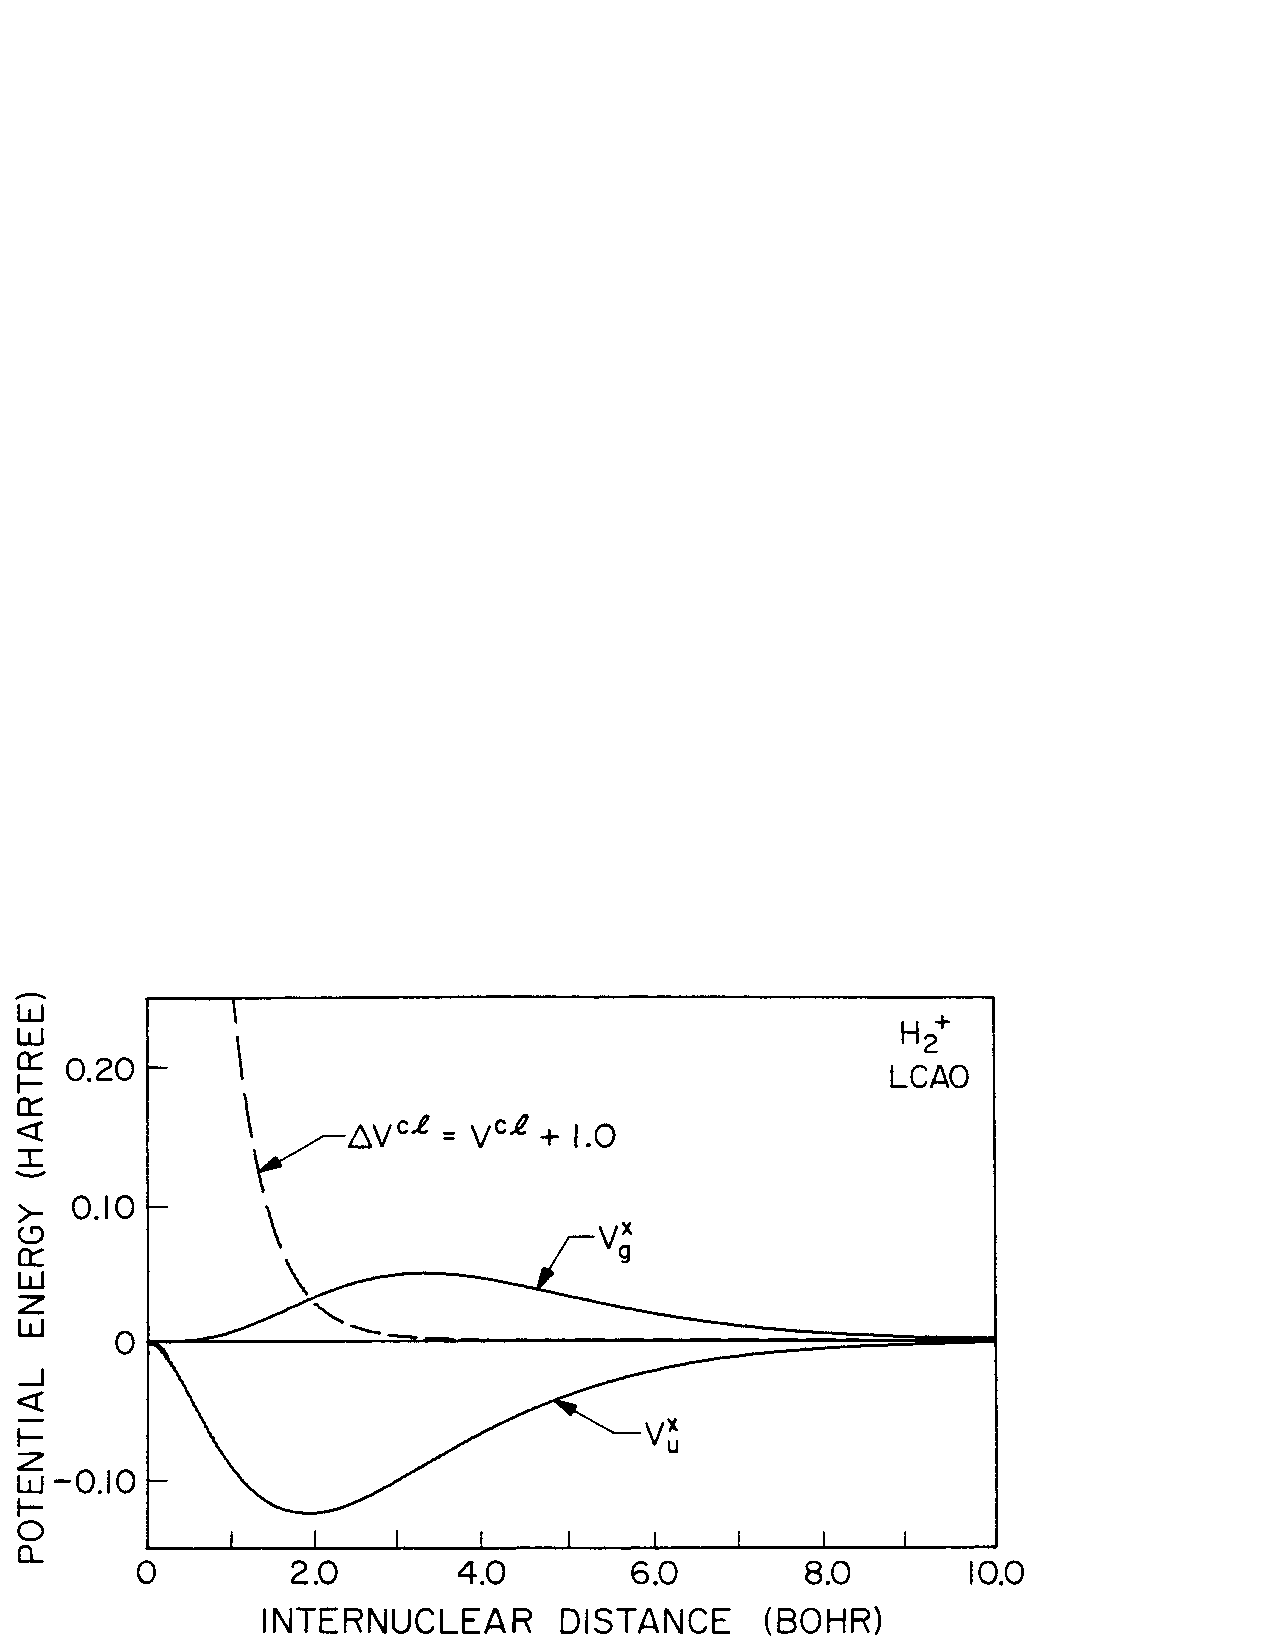
\includegraphics[scale=0.75]{fig2-36}
\caption{}
\label{fig2app-3}
\end{figure}

\subsubsection{The Kinetic Energy Terms}

The kinetic energy of the $\varphi_g$ state, can be written as
\begin{equation}
T_g = {t_{ll} + t_{rr} + 2t_{lr} \over 2(1+S)} = {t_{ll} + t_{lr} 
\over 1+S} ,
\end{equation}
where
\begin{equation}
t_{ll} = \langle \chi_\ell \vert {\hat t} \vert \chi_\ell \rangle = t_{rr} ,
\end{equation}
\begin{equation}
t_{lr} = \langle \chi_\ell \vert {\hat t} \vert \chi_r \rangle .
\end{equation}
We will write
\begin{equation}
T_g = T^{cl} + T^x_g ,
\end{equation}
where
\begin{equation}
T^{cl} = {1 \over 2} \left( t_{ll} + t_{rr} \right) = t_{ll}
\end{equation}
\begin{equation}
T^x_g = {t_{lr} - ST^{cl} \over 1+S} = {\tau_t \over 1+S}
\end{equation}
\begin{equation}
\tau_t = t_{lr} - ST^{cl}
\end{equation}
Similarly,
\begin{equation}
T_u = T^{cl} + T^x_u ,
\end{equation}
where
\begin{equation}
T^x_u = - {t_{lr} - ST^{cl} \over 1-S} = - {\tau_t \over 1-S}
\end{equation}
Since $T^{cl}$ is just the atomic value of the kinetic energy, 
independent of $R$, the changes in $T$ responsible for bonding must 
all be contained in $T^x$. Thus, the plots of $T_g$ and $T_u$ in
Figure \ref{fig2-7} are actually plots of $T^x_g$ and $T^x_u$.
    
The large negative value of $T_g$ responsible for the bond in H$^+_2$ results
from the large negative value of $\tau_t$.  We will now examine why 
$\tau_t$ is large and negative. We know that
\begin{equation}
t_{lr} = - {1 \over 2} \langle \chi_\ell \vert \nabla^2 \vert \chi_r 
\rangle = {1 \over 2} \langle \nabla \chi_\ell \cdot \nabla \chi_r 
\rangle = {1 \over 2} \int d \tau \left( \nabla \chi^*_\ell \right) 
\cdot \nabla \chi_r
\end{equation}
\begin{equation}
t_{ll} = {1 \over 2} \langle  \vert \nabla \chi_\ell \vert^2 \rangle ,
\end{equation}
\begin{equation}
t_{rr} = {1 \over 2} \langle  \vert \nabla \chi_\ell \vert^2 \rangle .
\end{equation}
Thus,
\begin{equation}
\tau_t = t_{lr} - {1 \over 2} S \left( t_{ll} + t_{rr} \right) =
{1 \over 2} \int d^3 {\bf r} \left\{ \nabla \chi_\ell \cdot \nabla 
\chi_r - {S \over 2} \left[ \left( \nabla \chi_\ell \right)^2 + \left( 
\nabla \chi_r \right)^2 \right] \right\}
\label{eqno2app-21}
\end{equation}
 
In order to understand the significance of the terms above, we will 
consider first the case where $\tau_t$ is modified by replacing 
$\nabla \chi_\ell \cdot \nabla \chi_r$ in the equation, by 
$\vert \nabla \chi_\ell \vert \vert \nabla \chi_r \vert$.  This leads to 
an integrand of the form
\begin{equation}
\vert \nabla \chi_r \vert \vert \nabla \chi_\ell \vert - {S \over 2} 
\left[ \left( \nabla \chi_\ell \right)^2 + \left( \nabla \chi_r 
\right)^2 \right] .
\label{eqno2app-22}
\end{equation}
Since
\begin{equation}
\chi_\ell = e^{-r_a}
\end{equation}
we obtain
\begin{equation}
\nabla \chi_\ell = - \chi_\ell {\hat e}_r ,
\end{equation}
where ${\hat e}_r$ is a unit vector in the $r$ direction, and hence,
(22) becomes
\begin{equation}
\left[ \chi_r \chi_\ell - {S \over 2} \left( \chi^2_\ell + \chi^2_r 
\right) \right]
\end{equation}
However, the term in brackets is just proportional to $\rho^x$ in
(\ref{eqno2app-19}) and hence, from (\ref{eqno2app-20}) the resulting
integral is zero. Thus, it is the difference between the dot product
term $\nabla \chi_\ell \cdot \nabla \chi_r$ in (\ref{eqno2app-21}) and
the absolute value term $\vert \nabla \chi_\ell \vert \vert \nabla
\chi_r \vert$ in (\ref{eqno2app-22}) that is responsible for the large
negative value of $\tau_t$; hence, of the chemical bond. To emphasize
this, we define a function called the contragradience
\begin{equation}
C ( {\bf r} ) = \vert \nabla \chi_\ell 
\vert \vert \nabla \chi_r \vert - \nabla \chi_\ell \cdot \nabla \chi_r
\end{equation}
such that
\begin{equation}
\tau_t - {1 \over 2} \int d^3 {\bf r} C ( {\bf r} ) .
\end{equation}
Large contragradiences lead to a laxge negative $\tau_t$, and hence,
strong bonds.  As discussed in the text and illustrated in Figure
\ref{fig2-14}, the larger values of $C( {\bf r})$ occur for points
in between the nuclei.

\subsubsection{Specific Results for H$^+_2$}

The explicit form of $\tau_t$ for H$^+_2$ is
\begin{equation}
\tau_t = - {1 \over 3} R^2 e^{-R}
\end{equation}
Thus, as expected $\tau_t \rightarrow 0$ as $R \rightarrow 0$ and as
$R \rightarrow \infty$. The minimum in $\tau_t$ occurs for $R =
2$. Thus, we would expect the maximum bonding effect to occur near $R
= 2\ a_0$.  Indeed this is the optimum $R$ of the exact wavefunction
of H$^+_2$. Approximating the bond strength as
\begin{equation}
T^x_g = - {\tau_t \over 1+S}
\end{equation}
we obtain for $R = 2$, where $S = 0.6$,
\begin{equation}
T^x_g = {4e^{-2} \over (3)(1.6)} = - 0.12\ h = 3.1\ \mathrm{eV}
\end{equation}
In fact, the bond energy is only $0.1\ h = 2.5$ eV, and the $T^x_g$ term 
does dominate the bond.  For quantitative considerations we should, of 
course, use the total $E^x$.

The explicit form of $\tau_v$ for H$^+_2$ is
\begin{equation}
\tau_v = e^{-R} \left[ {1 \over R} - {2 \over 3} R + {1 \over 3} R^2 
\right] ,
\end{equation}
neglecting terms of order $e^{-2R}$. Combining with $\tau_t$ leads to
\begin{equation}
\tau = e^{-R} \left[ {1 \over R} - {2 \over 3} R \right]
\end{equation}
neglecting terms of order $e^{-2R}$, whereas
\begin{equation}
S =  e^{-R} \left[ 1 + R + {1 \over 3} R^2 \right]
\end{equation}
Thus,
\begin{equation}
{\tau \over S} = - {2 \over R} \left( 1 - {3 \over R} + {9 \over 
2R^2} \right) + 0 \left( {1 \over R^4} \right)
\end{equation}
and, hence
\begin{equation}
\tau \approx - {2 \over R} S .
\end{equation}
Various energies for H$^+_2$ are tabulated in Table \ref{table-2-1}.

\begin{table}
\caption{Energy quantities for the linear combinations of 
atomic orbital wavefunctions of the $g$ state of H$^+_2$.  All
quantities are in atomic units.}
\label{table-2-1}

\begin{tabular}{cccccccc}\\ \hline
$R$ & $S$ & $\Delta V^{cl}$ & $V^x$ & $\Delta V^{tot}$ & $T^x = 
\Delta T^{tot}$ & $\Delta E^{tot}$\cr

$\infty$ & & O.O$^a$ & 0.0 & 0.0$^a$ & O.O$^a$ & O.O$^a$\cr
10.0&0.00201&0.00000&0.00121&0.00121&$-$0.00151&$-$0.00030\cr
8.0&0.01018&0.00000&0.00536&0.00536&$-$0.00708&$-$0.00173\cr
6.0&0.04710&0.00001&0.01933&0.01934&$-$0.02841&$-$0.00907\cr
5.0&0.09658&0.00005&0.03195&0.03200&$-$0.05120&$-$0.01920\cr
4.0&0.18926&0.00042&0.04485&0.04527&$-$0.08214&$-$0.03687\cr
3.5&0.25919&0.00117&0.04858&0.04975&$-$0.09792&$-$0.04817\cr
3.0&0.34581&0.00331&0.04837&0.05168&$-$0.11076&$-$0.05908\cr
2.5&0.45831&0.00943&0.04301&0.05244&$-$0.11727&$-$0.06483\cr
2.0&0.58645&0.02747&0.03250&0.05997&$-$0.11374&$-$0.05377\cr
1.5&0.72517&0.08298&0.01901&0.10199&$-$0.09700&+0.00499\cr
1.0&0.85839&0.27067&0.00695&0.27762&$-$0.06599&?0.21163\cr
0.5&0.96034&1.10364&0.00080&1.10443&$-$0.02578&?1.07865\cr
\hline
\end{tabular}
   
{$^a$} The values at $R = \infty$ are $V^{cl} = -1.00$, $V^{total} = 
-1.0$, $T^{total} = 0.5$, and $E^{total} = 0.5$.

\end{table}
